% !TeX program = pdflatex
\documentclass[a4paper,10pt,titlepage,twoside]{book}

% ==================================================
% UNITO thesis layout - Overleaf compatible version
% Main compiler: pdfLaTeX
% The original UNITO template uses fontspec/Tahoma and therefore may require
% LuaLaTeX. This version preserves the same title-page layout while compiling
% safely with the default Overleaf compiler.
% ==================================================

\usepackage[english]{babel}
\usepackage{iftex}

\ifPDFTeX
    \usepackage[T1]{fontenc}
    \usepackage[utf8]{inputenc}
    \usepackage{lmodern}
    \usepackage[scaled=0.95]{helvet}
    \newcommand{\CoverFont}{\sffamily}
\else
    \usepackage{fontspec}
    \IfFontExistsTF{Tahoma}{
        \newfontfamily\CoverFont[
            Scale=1,
            Ligatures=TeX,
            BoldFont={Tahoma Bold}
        ]{Tahoma}
    }{
        \newfontfamily\CoverFont[
            Scale=1,
            Ligatures=TeX
        ]{TeX Gyre Heros}
    }
\fi

\usepackage{xcolor}
\usepackage{graphicx}
\usepackage{array}
\usepackage{amsmath}
\usepackage{amsfonts}
\usepackage{amssymb}
\usepackage{amsthm}
\usepackage{tikz}
\usetikzlibrary{arrows.meta,positioning,shapes.geometric}
\usepackage{enumerate}
\usepackage{geometry}
\geometry{
    a4paper,
    top=3cm,
    bottom=3cm,
    left=3.5cm,
    right=3.5cm,
    heightrounded,
    bindingoffset=5mm
}
\usepackage{booktabs}
\usepackage{longtable}
\usepackage{listings}
\usepackage{emptypage}
\usepackage{indentfirst}
\usepackage{setspace}
\usepackage{microtype}
\singlespacing
\setlength{\parindent}{24pt}
\setlength{\emergencystretch}{2em}

\usepackage{xurl}
\usepackage[colorlinks=true,linkcolor=black,citecolor=black,urlcolor=blue]{hyperref}
\usepackage[nameinlink,noabbrev]{cleveref}
\usepackage[absolute]{textpos}

\numberwithin{equation}{chapter}
\renewcommand{\theequation}{\thechapter.\arabic{equation}}

% ==================================================
% Theorem-like environments retained from the UNITO template.
% They are available if needed in later chapters.
% ==================================================
\theoremstyle{plain}
\newtheorem{thm}{Theorem}[chapter]
\newtheorem{lem}[thm]{Lemma}
\newtheorem{cor}[thm]{Corollary}
\newtheorem{prop}[thm]{Proposition}

\theoremstyle{definition}
\newtheorem{defn}[thm]{Definition}
\newtheorem{ex}[thm]{Example}
\newtheorem{rmk}[thm]{Remark}
\newtheorem{notn}[thm]{Notation}

% ==================================================
% Source-code formatting
% ==================================================
\definecolor{codebackground}{RGB}{246,246,246}
\definecolor{codeframe}{RGB}{190,190,190}
\definecolor{codekeyword}{RGB}{30,70,150}
\definecolor{codecomment}{RGB}{60,115,60}

\lstdefinestyle{thesiscode}{
    backgroundcolor=\color{codebackground},
    frame=single,
    rulecolor=\color{codeframe},
    basicstyle=\ttfamily\small,
    keywordstyle=\color{codekeyword}\bfseries,
    commentstyle=\color{codecomment},
    numbers=left,
    numberstyle=\tiny,
    numbersep=8pt,
    breaklines=true,
    showstringspaces=false,
    tabsize=4,
    captionpos=b
}
\lstset{style=thesiscode}

% Inline long command-line options. Splitting the two leading hyphens prevents
% TeX from turning them into an en dash in ordinary text.
\newcommand{\cliopt}[1]{\texttt{-{}-#1}}

% ==================================================
% Thesis metadata
% Complete the fields marked with square brackets before submission.
% ==================================================
\newcommand{\UniversityName}{University of Turin}
\newcommand{\DegreeCourse}{Bachelor's Degree Program in Computer Science}
\newcommand{\ThesisTitleLineOne}{Design and Implementation of a}
\newcommand{\ThesisTitleLineTwo}{Simple Kathar\'a-Based Framework for}
\newcommand{\ThesisTitleLineThree}{Network Emulation and Testing}
\newcommand{\ThesisSubtitle}{Automated Topology Generation, Connectivity Validation and Denial-of-Service Experimentation}

\newcommand{\SupervisorName}{Prof.\ Gianluca Rizzo}
\newcommand{\CoSupervisorName}{[Name e Surname]}
\newcommand{\CandidateName}{Luca Bortoluzzi}
\newcommand{\StudentNumber}{Student ID: 1097723}
\newcommand{\AcademicYear}{2025/2026}

% Change to \ShowCoSupervisortrue if the final thesis has a co-supervisor.
\newif\ifShowCoSupervisor
\ShowCoSupervisorfalse

\begin{document}
\hypersetup{pageanchor=false}

% ==================================================
% Official-style UNITO title page
% ==================================================
\pagenumbering{gobble}
\thispagestyle{empty}

\begingroup
\CoverFont

\begin{textblock*}{4cm}(8.65cm,1.03cm)
    \centerline{
\includegraphics[width=3.67cm]{LogoUniToConvertito.png}}
\end{textblock*}

\begin{textblock*}{21cm}(0cm,8.98cm)
    \fontsize{18}{22}\selectfont
    \centerline{\textbf{\UniversityName}}
\end{textblock*}

\begin{textblock*}{21cm}(0cm,9.97cm)
    \fontsize{18}{22}\selectfont
    \centerline{\textit{\DegreeCourse}}
\end{textblock*}

\begin{textblock*}{19cm}(1cm,12.85cm)
    \fontsize{20}{24}\selectfont
    \centering
    \textbf{\ThesisTitleLineOne}\\
    \textbf{\ThesisTitleLineTwo}\\
    \textbf{\ThesisTitleLineThree}
\end{textblock*}

\begin{textblock*}{19cm}(1cm,15.58cm)
    \fontsize{15}{19}\selectfont
    \centering
    \textit{\ThesisSubtitle}
\end{textblock*}

\begin{textblock*}{21cm}(0cm,17.15cm)
    \fontsize{18}{22}\selectfont
    \centerline{\Large Bachelor's Thesis}
\end{textblock*}

\fontsize{14}{17}\selectfont

\begin{textblock*}{8cm}(3.04cm,18.60cm)
    \noindent
    \textbf{Supervisor}
\end{textblock*}
\begin{textblock*}{8cm}(3.04cm,19.19cm)
    \noindent
    \SupervisorName
\end{textblock*}

\ifShowCoSupervisor
    \begin{textblock*}{8cm}(3.04cm,20.64cm)
        \noindent
        \textbf{Correlatore/Correlatrice}
    \end{textblock*}
    \begin{textblock*}{8cm}(3.04cm,21.23cm)
        \noindent
        \CoSupervisorName
    \end{textblock*}
\fi

\begin{textblock*}{8cm}(12.33cm,22.95cm)
    \noindent
    \textbf{Candidate}
\end{textblock*}
\begin{textblock*}{8cm}(12.33cm,23.55cm)
    \noindent
    \textbf{\CandidateName}
\end{textblock*}
\begin{textblock*}{8cm}(12.33cm,24.14cm)
    \noindent
    \StudentNumber
\end{textblock*}

\begin{textblock*}{21cm}(0cm,27.34cm)
    \centerline{Academic Year \AcademicYear}
\end{textblock*}

\endgroup

\clearpage
\thispagestyle{empty}
\null
\clearpage

\TPoptions{absolute=false}
\pagestyle{plain}
\hypersetup{pageanchor=true}

% ==================================================
% Front matter
% ==================================================
\frontmatter
\pagenumbering{roman}

\chapter*{Declaration}
\phantomsection
\addcontentsline{toc}{chapter}{Declaration}

I declare to be responsible for the content I'm presenting in order to obtain
the final degree, not to have plagiarized in all or part of the work produced
by others, and to have cited original sources in a manner consistent with
current plagiarism regulations and copyright. I am also aware that, in case
of a false declaration, I could incur legal penalties and my admission to the
final exam could be denied.

\chapter*{Abstract}
\phantomsection
\addcontentsline{toc}{chapter}{Abstract}

Network laboratories are widely used to study routing, service deployment,
traffic analysis, and cybersecurity. Nevertheless, the manual preparation of
a network-emulation environment often requires several configuration files,
repeated commands, and careful coordination among topology, addressing,
routing, and application services. This thesis presents the design and
implementation of a lightweight Python-based framework built on top of
Kathar\'a. The framework allows a network laboratory to be described through a
structured YAML configuration containing nodes, interfaces, collision domains,
IP addresses, gateways, static routes, routing protocols, and optional
services. Starting from this declarative description, the system validates the
input and automatically generates the files required to deploy the
corresponding Kathar\'a laboratory. The project also includes an automated
validation component. Legitimate clients execute concurrent TCP connection
tests against a target service, while the framework records the result and the
elapsed time of every request in structured CSV files and execution logs. The
same procedure is applied to a baseline scenario and to a controlled
Denial-of-Service simulation executed inside an isolated laboratory. The
objective is not to replace Kathar\'a, but to provide a simple abstraction and
orchestration layer that reduces repetitive configuration tasks and supports
repeatable experiments. The resulting workflow integrates topology generation,
routing configuration, service deployment, traffic inspection, connectivity
testing, and the comparison of network behaviour under normal and adverse
conditions.

\bigskip
\noindent\textbf{Keywords:}
network emulation; Kathar\'a; Docker; YAML; FRRouting; automated testing;
Wireshark; denial of service; large language models.

\tableofcontents

\chapter*{Introduction}
\phantomsection
\addcontentsline{toc}{chapter}{Introduction}
\label{chap:introduction}

Computer networks are increasingly complex systems composed of heterogeneous
devices, protocols, and services. Even a limited experimental scenario can
include several end hosts, multiple routers, dynamic routing, a demilitarised
zone, traffic-monitoring tools, and one or more application services. Creating
such an environment requires not only a logical topology, but also a coherent
set of executable configurations.

Experimentation on physical hardware is not always practical. Dedicated
devices may be expensive or unavailable, while changes to existing equipment
may interfere with operational networks. Physical laboratories can also be
difficult to reproduce exactly. Network emulation addresses these limitations
by creating isolated environments in which real networking software can be
executed without requiring a separate physical device for every node
\cite{lantz2010network}.

Kathar\'a is an open-source, container-based network emulation system intended
for teaching, research, sandbox testing, and protocol development
\cite{kathara_website,scazzariello2020kathara,bonofiglio2018kathara}. It represents network devices as
containers and connects their virtual interfaces through Layer 2 collision
domains. This approach makes it possible to reproduce multi-node network
scenarios on a single workstation while retaining access to real protocol
stacks and routing software.

Although Kathar\'a reduces the infrastructure required for network
experiments, the creation of a laboratory still involves several files and
repetitive operations. The user must normally define the topology, prepare
startup files, assign addresses, configure gateways and routes, initialise
routing daemons, copy application scripts, and verify that the generated
environment behaves as expected.

These tasks become increasingly difficult to coordinate as the topology grows.
The same information may appear in several artefacts, and a modification to
one file may not be reflected in the others. A laboratory can also start
without immediately revealing an incorrect route, an inactive application
service, or an inconsistent address.

This thesis presents a framework that introduces a declarative configuration
layer above Kathar\'a. A network laboratory is described through a YAML file,
which is parsed and validated before the required Kathar\'a files are
generated. The framework supports several node roles, interface and gateway
configuration, static and dynamic routing, application services, optional
traffic inspection, and custom node commands.

The work also addresses functional validation. A dedicated testing component
discovers legitimate clients and performs simultaneous TCP connection attempts
against a selected service. Each attempt is classified according to the
application response and is recorded together with its elapsed time. The
results are stored in a form that can be aggregated and compared.

The framework is finally used to execute two phases across two related service
architectures. Each architecture is measured first under baseline conditions
and then while attacker-controlled nodes generate a bounded
Denial-of-Service workload. The first topology exposes the application server
directly; the second places a rate-limiting reverse proxy in front of a private
backend. Reusing the same client-side measurement procedure makes it possible
to observe both the effect of the additional workload and the outcome of the
mitigation in the tested configuration.

The implemented system was not obtained from a completely fixed specification
in a single development step. The project followed an iterative and incremental
software-development lifecycle. A further practical question arises from the
current use of LLM-based assistants in programming and network configuration:
which parts of the workflow can be delegated to a general-purpose LLM, and
which parts still benefit from an explicit domain-specific validator and
generator? This question is addressed explicitly in
\Cref{sec:llm-role} and revisited as a future integration direction in
\Cref{sec:future-llm-integration}. The development lifecycle began with the
narrower objective of reducing the repetitive preparation of Kathar\'a
laboratories and progressively acquired
new requirements as generated topologies were executed and inspected. Problems
observed during these iterations motivated the introduction of semantic
validation, richer routing support, optional diagnostic components, explicit
lifecycle management, application-level connectivity checks, concurrent
measurements, and finally robustness and scalability evaluation. The thesis
therefore discusses not only the final implementation, but also the reasons for
important design choices, the alternatives they replaced, and the limitations
revealed during verification.

\section*{Objectives}
\phantomsection
\addcontentsline{toc}{section}{Objectives}

The principal objectives of the work are:

\begin{itemize}
    \item to define a readable declarative format for network laboratories;
    \item to validate the configuration before generating deployment files;
    \item to automate the generation of Kathar\'a topology and startup files;
    \item to generate FRRouting configurations for supported routing
    protocols;
    \item to integrate optional packet inspection with Wireshark;
    \item to support deployment of node-specific application resources and
    startup commands;
    \item to execute concurrent application-level connectivity tests;
    \item to store reproducible, machine-readable experimental results;
    \item to compare normal service behaviour with behaviour under a
    controlled Denial-of-Service workload and evaluate a reverse-proxy
    mitigation using the same measurement procedure;
    \item to assess the role of the framework in an LLM-assisted network
    experimentation workflow and identify which responsibilities should remain
    deterministic and explicitly verifiable.
\end{itemize}

\section*{Research Questions}
\phantomsection
\addcontentsline{toc}{section}{Research Questions}

The thesis is guided by the following questions:

\begin{description}
    \item[RQ1] How can a declarative topology description be translated into
    the files and directories required by Kathar\'a?

    \item[RQ2] How can the generated laboratory automatically include
    addressing and routing configuration, deploy node-specific application
    resources and startup commands, and attach monitoring components?

    \item[RQ3] How can end-to-end service availability and application
    response time be measured repeatedly from several legitimate clients?

    \item[RQ4] Can the same workflow support a controlled comparison between
    baseline and Denial-of-Service conditions, and can it evaluate a
    reverse-proxy mitigation without changing the client measurement method?

    \item[RQ5] What additional value does a deterministic validation and
    generation framework provide when LLMs can already assist with network
    configuration, and how can the two approaches be combined in a practical
    experimentation workflow?
\end{description}

RQ1--RQ4 are answered through implementation evidence and experimental
evaluation. RQ5 is a design and discussion question addressed through
architectural analysis and comparison with the literature; this thesis does
not claim an empirical benchmark of LLM-generated configurations.

\section*{Thesis Structure}
\phantomsection
\addcontentsline{toc}{section}{Thesis Structure}

\Cref{chap:background} introduces network emulation and the supporting
technologies. \Cref{chap:requirements-architecture} defines the requirements,
reconstructs the development lifecycle of the project, presents the final
system architecture, and positions the framework relative to LLM-assisted
configuration. \Cref{chap:configuration-validation} describes the YAML model
and validation subsystem, including the implementation choices that emerged as
the configuration language evolved. The following chapters present laboratory
generation and lifecycle management, the experimental scenarios and results,
robustness and scalability evaluation, possible future developments---including
an LLM-assisted configuration front end---and the conclusions of the work.

% ==================================================
% Main matter
% ==================================================
\mainmatter

\chapter{Network Emulation and Supporting Technologies}
\label{chap:background}

\section{Chapter Overview}
\label{sec:chapter1-overview}

This chapter introduces the technical concepts and software technologies on
which the developed framework is based. The purpose is not to provide an
exhaustive description of each tool, but to identify the functions that each
technology performs in the proposed workflow. The framework combines
container-based execution, network emulation, declarative configuration,
dynamic routing, and packet inspection. These elements must cooperate while
remaining sufficiently transparent for the user to inspect and debug a
generated laboratory.

The chapter first discusses the role of experimental network environments and
the distinction between simulation and emulation. It then presents containers
and Docker as the execution substrate used by Kathar\'a. The Kathar\'a
laboratory model is described through nodes, interfaces, collision domains,
startup files, and node directories. The final sections introduce YAML,
FRRouting, Wireshark, and the role of automated validation in a reproducible
laboratory-generation process.

\section{Experimental Network Environments}
\label{sec:experimental-network-environments}

Network experimentation is required whenever a topology, protocol, service,
or configuration must be studied without modifying an operational network. A
small experiment may contain only two hosts and one router. A more complete
scenario may include several access networks, a routing core, a server
network, multiple routing protocols, and monitoring components. Reproducing
such a scenario on physical equipment is possible, but it introduces costs
and practical limitations.

Physical laboratories require dedicated devices, cabling, power, and space.
They also make repeated experiments more difficult because the initial state
must be restored before every execution. The configuration of one device may
remain from a previous test, while a replacement device may use a different
software version. These factors reduce reproducibility and make the
experimental procedure dependent on the available hardware.

Software-based environments address these limitations by representing network
nodes and links through processes, virtual machines, containers, or simulated
models. A complete topology can be stored as files, recreated on demand, and
shared with another user; container- and namespace-based emulation systems are
commonly used to support rapid and repeatable prototyping
\cite{lantz2010network,scazzariello2020kathara}. This approach is particularly appropriate for
educational and research activities, where the objective is often to inspect
the behaviour of protocols rather than to reproduce the exact performance of
physical hardware.

The use of a software environment does not remove the need for careful design.
Addresses, routes, interfaces, and services must still be mutually coherent.
Automation is therefore valuable not only because it reduces typing, but
because it makes it possible to derive several configuration artefacts from a
single description.

\section{Simulation and Emulation}
\label{sec:simulation-emulation}

The terms \emph{simulation} and \emph{emulation} are sometimes used
interchangeably, but they describe different approaches. A simulator models
the behaviour of a system through abstractions. Events such as packet
transmission, propagation delay, queueing, or protocol transitions are
represented by the simulation engine. The simulated node does not necessarily
execute the same software that would run on a real host or router.

An emulator instead provides an execution environment in which real network
stacks and applications can operate. The nodes may be implemented as virtual
machines, containers, namespaces, or other isolated processes, but they
execute real commands and exchange real packets. This gives the user access to
standard Linux tools and routing daemons.

The distinction affects the interpretation of results. Simulation is suitable
when the experiment requires controlled mathematical models, large synthetic
networks, or repeatable event timing. Emulation is useful when the experiment
focuses on configuration, interoperability, command-line behaviour, packet
formats, and software services. The framework developed in this thesis uses
emulation because its primary goal is to generate executable Kathar\'a
laboratories rather than abstract protocol models.

The use of emulation also explains why generated files remain important. A
laboratory is not only a graph of nodes and links. Each node must receive Linux
commands, files, and, where required, routing-daemon configuration. The
framework must therefore translate an abstract topology description into a
filesystem structure that can be executed by the emulator.

\section{Virtual Machines and Containers}
\label{sec:virtual-machines-containers}

Virtual machines and containers are two common mechanisms for creating
isolated execution environments. A virtual machine emulates or virtualises a
complete computer and normally runs its own operating-system kernel. This
provides strong isolation and makes it possible to run different operating
systems on the same host. The cost is a comparatively large memory footprint,
longer startup time, and additional management overhead.

Containers isolate processes while sharing the host kernel. Each container
can have its own filesystem view, process namespace, network namespace, and
resource limits \cite{docker_container,docker_overview}. Since a container does not normally boot a complete guest
kernel, it can be created and destroyed more quickly than a virtual machine.
This property is useful for network laboratories, where a topology can contain
many nodes that execute similar Linux environments.

Containers should not be interpreted as lightweight virtual machines in every
respect. Their execution model and isolation boundaries are different. For the
purposes of this thesis, however, the relevant property is that each container
can act as an independent network node. It can own virtual interfaces, an IP
routing table, processes, and configuration files. Multiple containers can
therefore represent hosts and routers on a single workstation.

Container-based emulation also supports rapid regeneration. When the source
configuration changes, the old laboratory can be stopped and a new set of
containers can be created from the updated files. This matches the intended
workflow of the framework: the YAML description is treated as the persistent
source, while the running containers are temporary instances.

\section{Docker as the Execution Substrate}
\label{sec:docker}

Docker is the container runtime used by Kathar\'a in the developed project
\cite{docker_overview}. A Docker image contains a filesystem and metadata from
which containers are created. A container is a running or stopped instance of an image
\cite{docker_container,docker_image}. Images make it possible to provide a
consistent set of tools across nodes, while containers provide isolated
runtime instances.

Two image categories are relevant to the generator. Ordinary end hosts use the
\texttt{kathara/base} image by default. Nodes that require routing functions
use \texttt{kathara/frr}. The generator may also accept an explicit image in
the YAML configuration, allowing a node to override the default selection.
This decision is implemented by considering both the declared node type and
the presence of an enabled FRRouting section.

Docker supplies the low-level execution environment, but the framework does
not directly create Docker networks or containers. That responsibility is
delegated to Kathar\'a. This separation avoids duplicating the emulator's
functionality. The framework generates standard Kathar\'a artefacts, and
Kathar\'a subsequently translates them into Docker operations.

This architecture has an additional advantage: the generated laboratory can
be inspected and started without using the Python generator again. Once the
files exist, standard Kathar\'a commands are sufficient to operate the
laboratory. The output therefore remains portable within the Kathar\'a
ecosystem.

\section{Kathar\'a}
\label{sec:kathara}

Kathar\'a is a container-based network emulation system designed for teaching,
research, protocol development, and controlled experimentation
\cite{kathara_website,scazzariello2020kathara,bonofiglio2018kathara}. It represents network devices as
containers and interconnects their interfaces through named Layer 2 collision
domains. A laboratory is stored as a directory whose files describe the
network and the configuration of each node \cite{kathara_manpage}.

\subsection{Nodes and Interfaces}
\label{subsec:kathara-nodes-interfaces}

A Kathar\'a node is identified by a name. The node can represent an end host,
a router, a firewall, a server, or another Linux-based device. Interface
indices are explicit in \texttt{lab.conf}: index 0 maps to \texttt{eth0},
index 1 to \texttt{eth1}, and so on \cite{kathara_labconf_manpage}. In this
framework, those indices are generated from the order of the interfaces in the
YAML list.

A topology entry has the following form:

\begin{lstlisting}[caption={Basic Kathar\'a interface declaration.},label={lst:kathara-interface}]
r1[0]="lan_a"
r1[1]="backbone"
\end{lstlisting}

The first line attaches \texttt{r1:eth0} to the collision domain
\texttt{lan\_a}. The second attaches \texttt{r1:eth1} to
\texttt{backbone}. Nodes that refer to the same collision-domain name are
connected at Layer 2.

The declaration does not assign an IP address. Layer 2 connectivity and Layer
3 configuration are deliberately separated. The topology file determines
which interfaces share a network segment, while startup commands configure
addresses and routes inside the containers.

\subsection{The lab.conf File}
\label{subsec:lab-conf}

The \texttt{lab.conf} file is the central topology file of a Kathar\'a
laboratory. In addition to interface declarations, it can contain laboratory
metadata and node properties such as the selected Docker image. The generator
produces entries such as:

\begin{lstlisting}[caption={Simplified generated lab.conf content.},label={lst:lab-conf-example}]
LAB_DESCRIPTION="Example routed laboratory"
LAB_VERSION=2.0
LAB_AUTHOR="Luca-Bortoluzzi"

pc_a[0]="lan_a"
pc_a[image]="kathara/base"

r1[0]="lan_a"
r1[1]="backbone"
r1[image]="kathara/frr"
\end{lstlisting}

This file is derived from the YAML node and interface declarations. The order
of interfaces in YAML determines the corresponding interface index in
\texttt{lab.conf}. Preserving this relationship is important because the
startup file assigns addresses to \texttt{eth0}, \texttt{eth1}, and the
subsequent interfaces in the same order.

\subsection{Startup Files}
\label{subsec:startup-files}

For a node named \texttt{r1}, Kathar\'a executes the commands stored in
\texttt{r1.startup} when the laboratory is started. Startup files commonly
configure addresses, default gateways, static routes, forwarding, and
services. A simplified file may contain:

\begin{lstlisting}[language=bash,caption={Simplified node startup file.},label={lst:startup-example}]
ip address add 10.10.1.1/24 dev eth0
ip address add 10.0.12.1/30 dev eth1
systemctl start frr
\end{lstlisting}

The generator writes one startup file for each node. It also appends custom
commands declared in YAML. This mechanism keeps common configuration
automatic while retaining an escape hatch for scenario-specific behaviour.

\subsection{Node Directories and hostlab}
\label{subsec:node-directories}

A directory with the same name as a node contains files that are made
available inside that node. In the project workflow, resources stored beside a
YAML configuration can be copied to the generated laboratory when the
\cliopt{import-dirs} option is used. A directory named \texttt{server}, for
example, is imported only if the YAML file declares a node named
\texttt{server}.

These resources can be accessed from the container through the laboratory
mount, commonly under \texttt{/hostlab}. This allows the startup file to
execute scripts that remain visible and editable on the host. The generator
excludes cache files and repository metadata so that generated laboratories do
not contain unnecessary development artefacts.

\subsection{Laboratory Lifecycle}
\label{subsec:kathara-lifecycle}

A generated laboratory is started with \texttt{kathara lstart} from its
directory. Kathar\'a reads \texttt{lab.conf}, creates the containers,
configures their interfaces, mounts node directories, and executes startup
files. A running node can be accessed using \texttt{kathara connect}.

The laboratory is stopped and removed from the runtime with
\texttt{kathara lclean}. The source files remain on disk and can be used for a
later execution \cite{kathara_manpage}. The project provides wrapper scripts for these operations;
their implementation and the complete generation lifecycle are discussed in
the following chapter.

\section{Declarative Configuration with YAML}
\label{sec:yaml-background}

YAML is a human-readable data-serialisation language frequently used for
configuration files \cite{yaml122}. It supports mappings, lists,
scalars, comments, and nested structures. These properties make it suitable
for representing a network laboratory in a form that is easier to maintain
than several independent startup and routing files.

A declarative description states the desired structure of the laboratory. It
does not require the user to write every command needed to create that
structure. The following fragment describes a host and a router:

\begin{lstlisting}[caption={Simplified YAML topology declaration.},label={lst:yaml-background-example}]
lab_name: example_lab

nodes:
  pc_a:
    type: host
    interfaces:
      - network: lan_a
        ip: 10.10.1.10/24
    default_gateway: 10.10.1.1

  r1:
    type: router
    interfaces:
      - network: lan_a
        ip: 10.10.1.1/24
      - network: backbone
        ip: 10.0.12.1/30
\end{lstlisting}

The same data are later translated into several outputs: interface entries in
\texttt{lab.conf}, address commands in startup files, a default route for the
host, and potentially routing configuration for the router. The YAML document
therefore becomes the persistent source of truth for generated files.

Using a structured input also enables validation. The framework can check
whether required fields exist, addresses are valid and unique, gateways belong
to a local subnet, and routing declarations refer to existing interfaces. The
validation process is a central subject of Chapter~\ref{chap:configuration-validation}.

\section{Dynamic Routing and FRRouting}
\label{sec:frrouting-background}

FRRouting, commonly abbreviated as FRR, is an open-source routing suite for
Linux and Unix systems. It provides implementations of protocols including
OSPF, RIP, and BGP \cite{frr_user_guide}. In the generated laboratories,
FRR allows containerised nodes to exchange routes dynamically and behave as
software routers.

FRR is organised around a set of protocol daemons and a common configuration
interface. The \texttt{daemons} file determines which processes are enabled.
The integrated \texttt{frr.conf} file contains protocol configuration, while
\texttt{vtysh} provides a unified command-line interface for inspection and
administration.

\subsection{OSPF}
\label{subsec:ospf-background}

Open Shortest Path First is a link-state interior gateway protocol. Routers
exchange topology information and compute paths within an autonomous routing
domain \cite{rfc2328}. The project supports both a common area declared at node level and an
\texttt{ospf\_area} marker associated with individual interfaces. This allows
simple single-area topologies and more structured multi-area configurations.

The generator can derive OSPF network statements from interface prefixes.
Validation verifies that explicitly declared OSPF networks overlap a locally
connected interface. This prevents a router from advertising a prefix that is
unrelated to its own configuration.

\subsection{RIP}
\label{subsec:rip-background}

Routing Information Protocol is a distance-vector protocol with a simpler
configuration model \cite{rfc2453}. In the project, the generator can enable the RIP daemon,
select the protocol version, disable automatic summarisation, and derive
network statements from node interfaces. RIP is useful for demonstrating that
the framework is not tied to one routing protocol.

\subsection{BGP}
\label{subsec:bgp-background}

Border Gateway Protocol exchanges reachability information between autonomous
systems \cite{rfc4271}. A BGP configuration requires an autonomous-system number, a router
identifier, one or more neighbours, and the prefixes to advertise. The
framework validates neighbour addresses, remote autonomous-system values, and
the existence of corresponding peer nodes.

The generated configuration includes two commands that are relevant in small
FRR laboratories: \texttt{no bgp ebgp-requires-policy} and
\texttt{no bgp network import-check}. Their use can be controlled through the
configuration model. They allow deliberately minimal educational topologies
to advertise prefixes without requiring additional policy definitions or an
already installed matching route. The policy-related behaviour is particularly
relevant to the default eBGP propagation model standardised in RFC~8212
\cite{rfc8212}.

\section{Traffic Inspection with Wireshark}
\label{sec:wireshark-background}

Wireshark is a network protocol analyser used to capture and inspect packets
\cite{wireshark_user_guide}. In an emulated environment it is useful for confirming
that packets traverse the expected collision domain, inspecting protocol
messages, and distinguishing routing failures from application failures.

The framework supports optional real-time Wireshark integration by adding a
dedicated node directly to \texttt{lab.conf}. The user can attach the node to
one or more selected collision domains. This is preferable to modifying an
existing host because monitoring remains separated from the logical role of
the emulated devices.

Packet capture is optional. A laboratory can be generated and executed without
Wireshark, while the same topology can later be regenerated with monitoring
enabled. This reflects a general design principle of the framework: diagnostic
features should not be mandatory components of every laboratory.

\section{Automation, Validation, and Reproducibility}
\label{sec:automation-reproducibility}

Automation is often described as a means of reducing manual effort, but its
more important contribution in this project is consistency. A manually edited
laboratory may contain a valid \texttt{lab.conf} and valid startup files that
nevertheless disagree with one another. A declarative generator can derive
both artefacts from the same interface list.

The framework applies two levels of validation before generation. Structural
validation verifies the minimum document shape required by the generator.
Semantic validation analyses relationships among nodes, interfaces, subnets,
gateways, and routing declarations. Errors stop generation, while warnings
identify suspicious but potentially intentional configurations.

Reproducibility depends on preserving the source configuration and generation
parameters. The generated laboratory is treated as a derived artefact. If a
persistent change is required, it should be made in the YAML file or in the
node resources stored under \texttt{configs/}, not only in the generated
\texttt{labs/} directory. A clean regeneration can then reconstruct the
laboratory from the maintained source.

\section{Positioning with Respect to Related Work}
\label{sec:related-work-positioning}

The framework combines ideas that are usually addressed separately in the
literature: executable network emulation, declarative configuration,
deterministic validation, and collection of application-level evidence. Its
contribution is not a new container runtime or routing suite. Rather, it is the
integration of these responsibilities around the standard Kathar\'a laboratory
format.

Mininet demonstrated that realistic network software could be used for rapid
prototyping on a single machine, with particular emphasis on software-defined
network experiments \cite{lantz2010network}. Kathar\'a provides the execution
substrate selected in this thesis and represents a broader range of Linux
network nodes through containers and collision domains
\cite{bonofiglio2018kathara,scazzariello2020kathara}. The developed framework
operates one level above Kathar\'a: it does not replace its runtime or file
format, but generates those files from a validated declarative source and adds
repeatable lifecycle and measurement operations.

A second line of work studies the use of LLMs for network configuration.
NetConfEval evaluates whether LLMs can perform network-configuration tasks,
while more recent work considers their role in zero-touch management and
surveys their wider use in network operations
\cite{wang2024netconfeval,lira2025llmnetcfg,liu2025llmnetworking}. These works
motivate natural-language assistance, but they also address a different
abstraction boundary. The present framework does not attempt to infer intent:
it receives explicit YAML and applies repeatable rules before producing an
executable laboratory. An LLM can therefore be used upstream as an optional
authoring aid, without becoming the authority that accepts a configuration.

\begin{table}[htbp]
\centering
\small
\setlength{\tabcolsep}{4pt}
\begin{tabular}{>{\raggedright\arraybackslash}p{0.16\textwidth}>{\raggedright\arraybackslash}p{0.25\textwidth}>{\raggedright\arraybackslash}p{0.25\textwidth}>{\raggedright\arraybackslash}p{0.22\textwidth}}
\toprule
\textbf{Approach} & \textbf{Scope and abstraction} & \textbf{Validation or evidence boundary} & \textbf{Relation to this work} \\
\midrule
Mininet \cite{lantz2010network} & Rapid prototyping, especially of SDN networks, through programmatic topologies and host/switch configuration & Experiment-specific correctness checks remain the responsibility of the experimenter & Alternative emulation approach; not the selected output target \\
Kathar\'a \cite{bonofiglio2018kathara,scazzariello2020kathara} & Container-based execution from laboratory files, startup scripts, and node resources & Consumes and executes its own laboratory representation & Runtime and file format used by the developed framework \\
LLM-based network configuration \cite{wang2024netconfeval,lira2025llmnetcfg,liu2025llmnetworking} & Translation of natural-language intent and assistance with operational tasks & Generated output remains candidate configuration requiring technical verification & Optional upstream authoring and diagnostic support \\
This thesis & Validated generation and repeatable evaluation from declarative YAML & Structural and semantic checks precede generation; runtime measurements test observable behaviour & Integration of source configuration, standard artefacts, lifecycle, and evidence \\
\bottomrule
\end{tabular}
\caption{Positioning of the developed framework relative to the main related approaches. The rows describe complementary scopes rather than a performance ranking.}
\label{tab:related-work-positioning}
\end{table}

The distinction in Table~\ref{tab:related-work-positioning} also limits the
claims of the thesis. The work does not compare emulator throughput, evaluate
LLM accuracy, or propose an alternative routing implementation. It evaluates
whether a narrow, explicit configuration model can coordinate existing tools,
reject recognised inconsistencies before generation, and support a controlled
experiment through a repeatable workflow.

\section{Chapter Summary}
\label{sec:chapter1-summary}

This chapter introduced the execution model and technologies used by the
framework. Container-based emulation provides isolated Linux network nodes,
Docker supplies the runtime, and Kathar\'a creates the topology from standard
laboratory files. YAML provides a declarative source representation,
FRRouting supplies dynamic routing, and Wireshark provides optional packet
inspection.

The chapter also established the distinction between source configuration and
generated artefacts. This distinction is central to the design of the system.
The next chapter translates the technological context into explicit
requirements, responsibilities, and architectural components.


\chapter{Requirements, Development Lifecycle and System Architecture}
\label{chap:requirements-architecture}

This chapter defines the problem addressed by the framework, its scope, its
requirements, the development lifecycle followed during the project, and the
architecture adopted by the final implementation. The framework accepts a YAML
configuration, validates it, and produces a standard Kathar\'a laboratory. It
also provides lifecycle scripts through which a generated laboratory can be
started, stopped, inspected, and removed. The detailed YAML model and the
validation rules are presented in Chapter~\ref{chap:configuration-validation},
while the translation of a valid configuration into \texttt{lab.conf}, startup
files, FRRouting files, and node resources is discussed in the following
chapter. The purpose of this chapter is therefore not only to state what the
framework does, but also to explain why its main components were introduced,
how problems encountered during development changed the requirements, and how
the resulting responsibilities cooperate as a single system.

\section{Problem, Scope, and Requirements}
\label{sec:problem-scope-requirements}

Kathar\'a provides a flexible representation of network laboratories
\cite{kathara_website,kathara_manpage}, but the configuration of a non-trivial
topology is normally distributed across several artefacts. A node interface is declared in \texttt{lab.conf}; its IP address is
assigned in a startup file; the corresponding prefix may appear again in an
FRRouting configuration; and scripts or other auxiliary resources may be
stored in the directory associated with the node. Each individual file is
readable, but the consistency of the complete laboratory must usually be
maintained manually.

This becomes progressively more difficult as the topology grows. A change to a
single address may require coordinated changes to a gateway, a routing
neighbour, an advertised network, a static route, or another reference used by
a node. The individual files may remain syntactically valid even when the
laboratory is no longer semantically coherent, and the resulting error may
only become visible after the emulated environment has started. Repetition is
a related problem: hosts repeatedly require interface configuration and a
default route, while routers repeatedly require interface addressing, an
appropriate container image, and routing configuration. Rewriting the same
information in multiple files increases the probability of inconsistent node
names, IP addresses, and interface indexes.

A further limitation of the standard file-based workflow is the absence of an
explicit validation boundary. Kathar\'a configuration files are executable
artefacts rather than a high-level schema that can be analysed before output
is written. The proposed framework introduces such a boundary by treating a
single declarative YAML document as the source configuration, validating that
document before generation, and only then producing the corresponding
Kathar\'a files. The general problem addressed by the work can therefore be
stated as follows:

\begin{quote}
How can a network laboratory be described once, checked for structural and
semantic consistency, translated into standard Kathar\'a artefacts, and
managed through a repeatable lifecycle?
\end{quote}

The framework is intentionally limited in scope. It does not replace Kathar\'a,
Docker, FRRouting, or Wireshark; instead, it acts as an automation layer that
prepares input for those tools. The implemented scope includes YAML-based
descriptions of laboratories, nodes, interfaces, addressing, gateways, static
routes, custom commands, and routing protocols; structural and semantic
validation before generation; generation of \texttt{lab.conf} and one startup
file per node; generation of FRRouting files for OSPF, RIP, and BGP; optional
import of directories associated with declared nodes; optional integration of
a real-time Wireshark node; explicit handling of pre-existing output
directories; shell wrappers for starting, stopping, and deleting laboratories;
and support for multiple configurations and generated laboratories. The
experimental components contained in the repository use these generated
laboratories, but they are not part of the core configuration architecture
discussed here; their workloads, measurements, and evaluation are addressed in
later chapters.

The primary user is a student, researcher, or network experimenter who already
understands basic Linux networking and needs to create repeatable Kathar\'a
laboratories. The framework does not hide networking concepts: the user still
chooses addresses, prefixes, gateways, routing protocols, and neighbours. Its
purpose is to avoid manually distributing the same design choices among many
files. A secondary stakeholder is the reviewer of an experiment. Generated
files must remain readable so that the relationship between the YAML source
and the resulting Kathar\'a configuration can be inspected. This requirement
motivates the generation of ordinary text files rather than the use of a
private runtime data store. The expected execution environment is a Linux
workstation with Python, PyYAML, Docker, and Kathar\'a installed
\cite{pyyaml_docs,docker_overview,kathara_website}. FRRouting is
provided by the appropriate Kathar\'a image, while Wireshark integration also
requires the selected container image and support for the exposed interface.

The resulting workflow can be summarised through a small set of principal use
cases. The user may select a configuration by supplying either an explicit
path or a configuration name resolved inside a configured search directory.
The framework then loads the document with PyYAML and requires the top-level
value to be a mapping. The user may validate the configuration without
creating or modifying a laboratory: structural validation checks mandatory
fields, while semantic validation checks relationships among addresses,
collision domains, gateways, roles, and routing declarations, producing a
report containing errors, warnings, and summary lines. After successful
validation, the user may generate the laboratory under the selected output
directory; the framework writes \texttt{lab.conf}, one startup file per node,
and the required FRRouting files, while existing output is handled according
to the selected \cliopt{force} or \cliopt{clean} behaviour. If directory
import is enabled, a directory located beside the YAML source is copied only
when its name matches a declared node; unmatched directories are reported as
warnings and skipped. Wireshark can be disabled, selected interactively,
attached directly to one or more collision domains, or associated with the
networks connected to a specific node. Finally, the generated laboratory can
be started, inspected, cleaned, and removed without deleting the original YAML
configuration.

These use cases are formalised by the following functional requirements.

\begin{longtable}{p{0.12\textwidth}p{0.78\textwidth}}
\caption{Functional requirements of the framework.}
\label{tab:functional-requirements}\\
\toprule
\textbf{ID} & \textbf{Requirement} \\
\midrule
\endfirsthead
\toprule
\textbf{ID} & \textbf{Requirement} \\
\midrule
\endhead
FR1 & The framework shall accept either an explicit YAML path or a configuration name resolved inside a configurable directory. \\
FR2 & The framework shall load YAML through a safe parser and reject a top-level value that is not a mapping. \\
FR3 & The framework shall require a laboratory name and a non-empty node mapping. \\
FR4 & The framework shall validate identifiers, node types, interfaces, collision domains, addresses, gateways, and routing declarations. \\
FR5 & The framework shall distinguish generation-blocking errors from non-blocking warnings. \\
FR6 & The framework shall provide a validation-only mode that does not create or modify a laboratory. \\
FR7 & The framework shall generate a Kathar\'a \texttt{lab.conf} file from node-interface declarations. \\
FR8 & The framework shall select a default container image according to node capabilities and permit an explicit image override. \\
FR9 & The framework shall generate one startup file for every declared node. \\
FR10 & Startup generation shall support interface addresses, a default gateway, static routes, FRR startup, and custom commands. \\
FR11 & The framework shall generate FRRouting daemon and configuration files for enabled FRR devices. \\
FR12 & The framework shall support OSPF, RIP, and BGP configuration forms represented by the YAML model. \\
FR13 & The framework shall optionally copy node directories located beside the source YAML file. \\
FR14 & The framework shall optionally attach a Wireshark node to selected collision domains. \\
FR15 & The framework shall avoid silently overwriting an existing laboratory unless the user selects an explicit overwrite or clean-regeneration option. \\
FR16 & The framework shall support a configurable output directory containing multiple generated laboratories. \\
FR17 & The project shall provide commands or wrappers to start, stop, inspect, and delete generated laboratories. \\
\bottomrule
\end{longtable}

In addition to these functions, the framework is constrained by a set of
non-functional requirements that influence both the architecture and the
implementation style.

\begin{longtable}{p{0.22\textwidth}p{0.68\textwidth}}
\caption{Non-functional requirements of the framework.}
\label{tab:non-functional-requirements}\\
\toprule
\textbf{Property} & \textbf{Requirement} \\
\midrule
\endfirsthead
\toprule
\textbf{Property} & \textbf{Requirement} \\
\midrule
\endhead
Reproducibility & The same maintained source configuration should regenerate the same logical laboratory structure. \\
Transparency & Generated files must remain ordinary, readable Kathar\'a and FRRouting artefacts. \\
Safety of file operations & Existing laboratory directories must not be removed or overwritten implicitly. \\
Modularity & Loading, validation, generation, monitoring selection, and lifecycle operations should have separate responsibilities. \\
Extensibility & New configuration properties or protocol forms should be addable without replacing the entire generation pipeline. \\
Usability & Common operations should be available through a command-line interface with explicit options and informative messages. \\
Traceability & Validation messages should identify the affected node, interface, domain, neighbour, or field. \\
Portability & The project should operate in a standard Linux, Python, Docker, and Kathar\'a environment. \\
Maintainability & Persistent modifications should be made in source YAML or resource directories rather than only in generated output. \\
Compatibility & The generated laboratory should remain operable with standard Kathar\'a commands. \\
\bottomrule
\end{longtable}

\subsection*{Requirements Traceability and Verification}
\phantomsection
\label{sec:functional-requirements-traceability}

Table~\ref{tab:functional-requirements-traceability} links each functional
requirement to the implementation behaviour and to the evidence presented in
the thesis. ``Verified'' denotes that the behaviour is demonstrated by the
described validation or generation workflow and, where applicable, by
execution of generated laboratories. It does not imply exhaustive testing of
every possible input combination.

\begin{longtable}{p{0.08\textwidth}p{0.64\textwidth}p{0.16\textwidth}}
\caption{Traceability matrix for functional requirements FR1--FR17.}
\label{tab:functional-requirements-traceability}\\
\toprule
\textbf{ID} & \textbf{Implementation and verification evidence} & \textbf{Assessment} \\
\midrule
\endfirsthead
\toprule
\textbf{ID} & \textbf{Implementation and verification evidence} & \textbf{Assessment} \\
\midrule
\endhead
FR1 & Path and configuration-name resolution are described in Section~\ref{sec:configuration-model-purpose} and exercised by the generation workflow. & Verified \\
FR2 & Safe YAML loading and rejection of a non-mapping root are part of the structural-validation boundary in Section~\ref{sec:structural-validation}. & Verified \\
FR3 & Mandatory \texttt{lab\_name} and non-empty \texttt{nodes} checks are documented with the structural rules in Section~\ref{sec:structural-validation}. & Verified \\
FR4 & Identifier, role, interface, addressing, gateway, collision-domain, and routing checks are described in Sections~\ref{sec:structural-validation} and~\ref{sec:validation-workflow}. & Verified \\
FR5 & The error/warning policy and its effect on generation are reported in Table~\ref{tab:error-warning-policy}. & Verified \\
FR6 & Validation-only execution terminates before output generation, as described in Section~\ref{sec:validation-workflow}; the large invalid stress case also produced no files in Section~\ref{sec:stress-methodology}. & Verified \\
FR7 & Translation from interface declarations to \texttt{lab.conf} is shown in Section~\ref{sec:generated-laboratory-structure} and Table~\ref{tab:yaml-to-generated}. & Verified \\
FR8 & Capability-based default-image selection and explicit overrides are documented in Sections~\ref{sec:laboratory-generation-process} and~\ref{sec:generated-laboratory-structure}. & Verified \\
FR9 & Per-node startup-file generation is described and illustrated in Section~\ref{sec:generated-laboratory-structure}. & Verified \\
FR10 & Generated address, gateway, route, FRR-startup, and custom-command entries are mapped in Table~\ref{tab:yaml-to-generated}. & Verified \\
FR11 & Generation of \texttt{daemons} and \texttt{frr.conf} for FRR-enabled nodes is described in Section~\ref{sec:generated-laboratory-structure}. & Verified \\
FR12 & The supported OSPF, RIP, and BGP forms and their validation are documented in Sections~\ref{sec:configuration-model-purpose} and~\ref{sec:structural-validation}; routed laboratories provide runtime use evidence. & Verified \\
FR13 & Selective import of directories whose names match declared nodes is described in Sections~\ref{sec:laboratory-generation-process} and~\ref{sec:generated-laboratory-structure}. & Verified \\
FR14 & Wireshark selection, generated attachment, and a runtime capture are presented in Section~\ref{sec:generated-laboratory-structure} and Figure~\ref{fig:wireshark-runtime-capture}. & Verified \\
FR15 & Refusal, explicit overwrite, and clean-regeneration behaviours are documented in Section~\ref{sec:laboratory-generation-process}. & Verified \\
FR16 & Output-root selection and coexistence of named generated laboratories are described in Sections~\ref{sec:laboratory-generation-process} and~\ref{sec:laboratory-lifecycle}. & Verified \\
FR17 & Start, stop, status, connection, clean, and deletion operations and their effects are reported in Section~\ref{sec:laboratory-lifecycle} and Table~\ref{tab:lifecycle-effects}. & Verified \\
\bottomrule
\end{longtable}

The matrix makes two boundaries explicit. First, FR12 is verified only for the
protocol forms represented by the current YAML model, not for every command
offered by FRRouting. Second, runtime execution complements but does not replace
static verification: opaque custom commands and complete manual FRR fragments
remain outside the semantics that the validator can prove.

\section{Software Development Lifecycle and Design Evolution}
\label{sec:software-development-lifecycle}

The final architecture should not be interpreted as the implementation of a
complete specification that existed before coding began. Development followed
an iterative and incremental lifecycle in which a small working solution was
extended after each cycle of generation, execution, observation, and
correction. This approach was appropriate for the project because several
requirements only became evident when real Kathar\'a laboratories were produced
and executed. In particular, failures that were invisible at the level of YAML
syntax or generated text files often became apparent only when routes,
services, or measurement scripts were exercised at runtime.

The initial requirement was deliberately narrow. Manually preparing a
Kathar\'a laboratory required the same design information to be distributed
among \texttt{lab.conf}, node startup files, FRRouting configuration, and
node-specific directories. One possible approach would have been to automate
edits to these files individually, but that would have preserved the very
duplication that motivated the project. A single declarative source was
therefore preferred. YAML was selected because its hierarchical structure maps
naturally to laboratories, nodes, interfaces, and nested routing properties,
while remaining readable and directly editable. The first useful prototype
could consequently describe a topology at a higher level and derive ordinary
Kathar\'a files from it.

Generation alone soon proved insufficient. A YAML document could be parsed and
translated while still describing an inconsistent network: for example, an
address could be duplicated, a default gateway could lie outside every local
subnet, or a routing relationship could refer to the wrong peer. Allowing such
configurations to reach the runtime moved deterministic errors to a much later
and less convenient debugging stage. Validation therefore became an explicit
architectural responsibility. Structural validation was introduced to protect
the implementation from malformed document shapes, while semantic validation
was added to reason about relationships among addresses, collision domains,
gateways, node roles, and routing declarations before any output was written.

The next iterations were driven by increasingly complex routed laboratories.
Simple host--router scenarios required only interfaces and gateways, whereas
multi-area OSPF, RIP, and multi-AS BGP scenarios required protocol-specific
identifiers, areas, autonomous-system numbers, neighbours, advertised prefixes,
and redistribution rules. Rather than replacing the earlier configuration
files whenever the representation grew, the implementation retained compatible
forms where practical. This reduced disruption to already working laboratories
and made them useful as regression inputs, at the cost of some redundancy in
the accepted FRRouting syntax. The same pragmatic principle motivated escape
mechanisms such as \texttt{commands} and \texttt{frr.config}: they allowed the
project to express specialised behaviour without first modelling every Linux or
FRRouting command in the declarative language.

Execution of the generated laboratories then introduced a different class of
requirements. Inspecting files was not enough to determine whether packets were
actually following the intended path or whether an application was available.
Optional Wireshark integration was added as a diagnostic aid, lifecycle
operations were kept separate from generation, and connectivity testing was
progressively extended from basic reachability towards application-level
verification. During development, a reachable target could still fail a service
test when the application process was not running; this made the distinction
between network reachability and service availability explicit in the final
measurement design. Similarly, sequential client tests were adequate for
checking individual hosts but were unsuitable once several clients had to
observe the same service condition. The test runner was therefore changed to a
round-based concurrent model.

The experimental phase continued the same feedback loop. Earlier runs showed
that application measurements could be contaminated by a network that had not
yet reached a usable routing state. This motivated explicit readiness checks
before collecting the baseline. As the repository accumulated several
configurations and generated laboratories, utilities were also adapted to avoid
assuming that only one laboratory existed and to use explicit targets or node
names where appropriate. Finally, after functional behaviour was stable enough
to support the controlled DoS experiment, development moved to verification of
the translator itself. The stress and robustness tests in
Chapter~\ref{chap:robustness-security-scalability} exposed new trade-offs,
including duplicated validation work, permissive unknown YAML keys, incomplete
analysis of arbitrary static routes, and the scalability cost of collision-domain
overlap checks.

Figure~\ref{fig:development-lifecycle} summarises the lifecycle used throughout
the project. Verification is not represented as a terminal activity: an
observed problem can create a new or refined requirement and start another
iteration.

\begin{figure}[htbp]
\centering
\begin{tikzpicture}[
    node distance=8mm and 14mm,
    state/.style={draw, rounded corners, align=center, minimum width=3.5cm, minimum height=8mm, font=\small},
    arrow/.style={-{Latex[length=2mm]}, thick}
]
\node[state] (need) {Problem or\\new requirement};
\node[state, right=of need] (design) {Design choice\\and alternative analysis};
\node[state, below=of design] (impl) {Implementation\\or refactoring};
\node[state, left=of impl] (verify) {Laboratory execution\\and verification};
\node[state, below=of verify] (observe) {Problem, limitation,\\or new need observed};

\draw[arrow] (need) -- (design);
\draw[arrow] (design) -- (impl);
\draw[arrow] (impl) -- (verify);
\draw[arrow] (verify) -- (observe);
\draw[arrow] (observe.west) -| ++(-1.0,0) |- (need.west);
\end{tikzpicture}
\caption{Iterative software-development lifecycle followed by the project.}
\label{fig:development-lifecycle}
\end{figure}

The main iterations can be related directly to concrete features of the final
framework, as summarised in Table~\ref{tab:development-evolution}. The table is
not intended as a strict chronological log of every code change; instead, it
identifies the recurring engineering pattern that connected requirements,
observed problems, and implementation decisions.

{\small
\begin{longtable}{>{\raggedright\arraybackslash}p{0.18\textwidth}>{\raggedright\arraybackslash}p{0.34\textwidth}>{\raggedright\arraybackslash}p{0.38\textwidth}}
\caption{Main development iterations and resulting design choices.}
\label{tab:development-evolution}\\
\toprule
\textbf{Development stage} & \textbf{Need or problem observed} & \textbf{Resulting design or feature} \\
\midrule
\endfirsthead
\toprule
\textbf{Development stage} & \textbf{Need or problem observed} & \textbf{Resulting design or feature} \\
\midrule
\endhead
Initial prototype & Repetitive and duplicated information across several Kathar\'a artefacts. & A declarative YAML source from which standard Kathar\'a files are generated. \\
Validation & Generated files could remain syntactically plausible while describing an incoherent network. & Separate structural and semantic validation before filesystem modification. \\
Routing extension & Larger laboratories required OSPF, RIP, BGP, multi-area, and multi-AS information. & Protocol-aware validation and FRRouting generation, while retaining compatible declaration forms. \\
Extensibility & Some node behaviour could not be represented by the current declarative fields. & Generic \texttt{commands}, imported node resources, and the \texttt{frr.config} escape mechanism. \\
Runtime diagnosis & Static inspection did not show actual packet paths or all runtime failures. & Optional Wireshark integration and explicit post-start inspection with Linux and FRR tools. \\
Service verification & A reachable host or open TCP port did not necessarily mean that the application completed the requested operation. & Application-level request validation and distinct ICMP, TCP, and application metrics. \\
Concurrent testing & Sequential client execution observed the service at different times. & Round-based concurrent measurements across legitimate clients. \\
Experiment orchestration & Early measurements could begin before the routed topology was ready. & Readiness checks, isolated experiment outputs, and explicit baseline/adverse phases. \\
Final verification & Functional success did not reveal all robustness or scalability limits. & Stress testing and analysis of permissive or expensive implementation choices. \\
\bottomrule
\end{longtable}
}

\section{System Architecture and Repository Organisation}
\label{sec:system-architecture-repository}

The architecture is organised as a sequential pipeline with explicit
responsibility boundaries. Figure~\ref{fig:framework-architecture} shows the
main flow from source configuration to the running laboratory.

\begin{figure}[htbp]
\centering
\begin{tikzpicture}[
    node distance=0.55cm,
    box/.style={rectangle,draw,rounded corners,minimum width=11cm,minimum height=0.85cm,align=center}
]
\node[box] (source) {YAML source configuration and optional node-resource directories};
\node[box,below=of source] (loader) {Path resolution and safe YAML loading (\texttt{Lexer.py})};
\node[box,below=of loader] (structure) {Structural validation (\texttt{Parser.py})};
\node[box,below=of structure] (semantic) {Semantic validation and validation report (\texttt{Parser.py})};
\node[box,below=of semantic] (generation) {Kathar\'a and FRRouting generation (\texttt{gen\_lab.py})};
\node[box,below=of generation] (output) {Generated laboratory under \texttt{labs/<lab\_name>/}};
\node[box,below=of output] (lifecycle) {Start, inspect, clean, and remove through Kathar\'a and wrapper scripts};

\draw[-{Latex[length=3mm]}] (source) -- (loader);
\draw[-{Latex[length=3mm]}] (loader) -- (structure);
\draw[-{Latex[length=3mm]}] (structure) -- (semantic);
\draw[-{Latex[length=3mm]}] (semantic) -- (generation);
\draw[-{Latex[length=3mm]}] (generation) -- (output);
\draw[-{Latex[length=3mm]}] (output) -- (lifecycle);
\end{tikzpicture}
\caption{High-level architecture of the laboratory-generation framework.}
\label{fig:framework-architecture}
\end{figure}

The pipeline does not construct a persistent hierarchy of domain objects such
as \texttt{Node} or \texttt{Interface} classes. Introducing a typed internal
model was considered a possible way to make invariants more explicit, but it
would also have added another conversion layer between YAML and the relatively
compact output model required by the prototype. The implemented version
therefore keeps the validated configuration as a nested combination of Python
dictionaries and lists. This choice reduced implementation overhead and made
new YAML properties easy to prototype, but it also means that the validator is
responsible for establishing all assumptions later used by the generator. The
limitations of this choice become visible again in the discussion of strict
schemas and unknown keys in Chapter~\ref{chap:robustness-security-scalability}.

The root-level \texttt{generate\_lab.py} file is intentionally minimal: it
imports and invokes \texttt{main()} from
\texttt{src\_gen\_lab/gen\_lab.py}. Configuration discovery and
deserialisation are handled by \texttt{Lexer.py}. Despite its historical
filename, this component does not perform token-by-token lexical analysis; its
architectural role is to resolve the supplied configuration and load YAML.
\texttt{Parser.py} performs the minimum structural checks and the complete
semantic analysis. It defines the supported node and protocol sets, the
identifier pattern, the validation issue representation, and the report used
by both validation-only and normal generation modes. The generation module,
\texttt{gen\_lab.py}, then selects node images, generates \texttt{lab.conf},
writes startup files, creates FRRouting configuration, copies matching
resource directories, integrates Wireshark when requested, and reports how the
resulting laboratory can be started and stopped.

Lifecycle management is intentionally kept outside the generator itself.
\texttt{start.sh} verifies that the supplied laboratory directory exists,
changes to that directory, and executes \texttt{kathara lstart}.
\texttt{stop.sh} performs the corresponding \texttt{kathara lclean}, while
\texttt{del\_lab.sh} removes one generated directory or, when explicitly
requested, the contents of the laboratory output directory. This separation
keeps generation, runtime management, and filesystem deletion as distinct
operations.

The repository contains both the core framework and the later experimental
components. The following view includes only the files relevant to the
configuration, generation, and lifecycle architecture discussed in the first
part of the thesis.

\begin{lstlisting}[caption={Repository structure relevant to the framework core.},label={lst:repository-structure}]
Thesis/
|-- configs/
|   |-- Test1.yml
|   |-- Test_enterprise_multi_as_structured.yml
|   |-- client-router-server.yml
|   |-- dos_lab.yml
|   |-- mitigation.yml
|   |-- multi-area.yml
|   `-- multi_AS.yml
|-- src_gen_lab/
|   |-- Lexer.py
|   |-- Parser.py
|   |-- __init__.py
|   `-- gen_lab.py
|-- labs/
|-- generate_lab.py
|-- start.sh
|-- stop.sh
|-- del_lab.sh
`-- README.md
\end{lstlisting}

The \texttt{configs/} directory is the persistent source area. It contains YAML
topologies and may also contain directories whose names match declared nodes.
The \texttt{src\_gen\_lab/} package contains the implementation, whereas
\texttt{labs/} contains generated output and is intentionally not expanded in
the source-tree representation. This organisation expresses an important
architectural distinction: source configuration is maintained independently
from generated files and from the runtime state of the laboratory.

\section{Operational Flow and Design Principles}
\label{sec:operational-flow-design}

The control flow begins when the user invokes the command-line entry point.
The argument parser collects the requested configuration, the input and output
directories, overwrite behaviour, validation mode, resource-import option, and
Wireshark selection. The configuration path is then resolved. If the supplied
argument already exists as a path, it is used directly; otherwise, the loader
searches the configured directory for matching \texttt{.yml} and
\texttt{.yaml} files. The YAML content is deserialised into ordinary Python
objects.

Structural validation runs before semantic analysis so that subsequent
functions do not have to operate on a document that lacks mandatory elements
such as \texttt{nodes} or \texttt{interfaces}. Semantic validation then checks
the relationships inside the model and deliberately collects all detectable
errors and warnings instead of stopping at the first issue. If at least one
error exists, generation is not started. If validation succeeds and
\cliopt{validate-only} is active, the process terminates without modifying
the filesystem. Otherwise, the generator prepares the selected output
directory and writes all derived artefacts.

The generated directory is independent from the running state. Generation
creates files; starting the laboratory creates containers and collision
domains; stopping it removes the runtime environment; deleting the generated
directory is yet another separate operation. Keeping these stages distinct
prevents the project from conflating the declarative source, the generated
representation, and the executing instance.

Several design principles follow directly from this flow. First, the YAML
file is treated as the declarative source of truth for topology and common
node configuration. Generated files are derived output, which reduces
duplication and allows the laboratory to be recreated through clean
generation. Second, the framework deliberately generates standard Kathar\'a
files instead of controlling containers directly through the Docker API or a
private orchestration layer. Direct Docker control would have provided more
runtime control, but it would also have duplicated responsibilities already
implemented by Kathar\'a and tied the project to its own execution path. By
generating ordinary Kathar\'a artefacts, the framework remains an input and
validation layer rather than a replacement runtime; the output stays
compatible with the normal Kathar\'a workflow and can be inspected or executed
manually \cite{kathara_manpage}.

Validation is also deliberately placed before filesystem modification. A
structural or semantic error should not leave a partially generated
laboratory, and the validation-only option makes the same checks available for
manual review or automated workflows. Destructive operations follow the same
principle of explicitness: an existing laboratory directory is not silently
replaced. The user must select \cliopt{force} to write into existing output
or \cliopt{clean} to remove and recreate it, making the potentially-
destructive behaviour visible at the command line.

Resource import uses a convention rather than an additional mapping file. A
node-specific directory is associated with a node when their names match. This
choice is simple and readable, but it creates a deliberate naming convention;
when import checking is enabled, directories that do not match declared nodes
are reported and skipped. Diagnostics are likewise optional rather than
mandatory. Wireshark integration can be disabled non-interactively, while the
user may attach the monitoring node only to the collision domains required for
debugging or inspection. The core topology can therefore be generated without
monitoring, and observation can be added only when needed.

Together, these decisions support the non-functional objectives identified in
Section~\ref{sec:problem-scope-requirements}. Reproducibility is obtained by maintaining the YAML
source and regenerating output from it; transparency and compatibility are
preserved through ordinary Kathar\'a and FRRouting files; safety is improved by
validation-first and explicit overwrite semantics; modularity is reflected in
the separation among loading, validation, generation, monitoring selection,
and lifecycle operations; and traceability is provided by validation messages
that refer to the affected node, interface, collision domain, neighbour, or
field.


\section{LLM-Assisted Configuration and Deterministic Validation}
\label{sec:llm-role}

General-purpose LLMs can assist with configuration authoring, but authoring,
validation, and experiment execution are distinct responsibilities. The
relevant question is therefore not whether an LLM can emit configuration text,
but which guarantees are required before that text is used in a repeatable
experiment. In this thesis, RQ5 is addressed as a design and discussion
question through architectural analysis and comparison with the literature;
no empirical benchmark of LLM-generated configurations is claimed.

An LLM can translate informal intent into a candidate topology, allocate
addresses, draft startup commands, produce FRRouting fragments, or create the
YAML source accepted by the framework. Recent studies examine these
capabilities in network configuration and intent-based management
\cite{wang2024netconfeval,lira2025llmnetcfg,liu2025llmnetworking}. Such output
is nevertheless candidate input rather than evidence that all addresses,
gateways, routing relationships, node names, and cross-file references satisfy
the laboratory invariants.

The framework provides the complementary deterministic boundary. It applies
the same structural and semantic checks on every invocation, derives
coordinated Kathar\'a and FRRouting artefacts from one validated representation,
and connects the generated laboratory to runtime measurements. This separation
is important because technically plausible generated output may still contain
functional or security weaknesses and therefore requires explicit checking
\cite{pearce2022copilotsecurity}. The comparison in
Table~\ref{tab:llm-framework-roles} summarises these complementary roles.

\begin{table}[htbp]
\centering
\small
\begin{tabular}{p{0.23\textwidth} p{0.32\textwidth} p{0.32\textwidth}}
\toprule
\textbf{Activity} & \textbf{Typical LLM contribution} & \textbf{Framework contribution} \\
\midrule
Expressing a network requirement & Accepts natural-language intent and can ask or answer clarifying questions. & Requires an explicit YAML representation; it does not interpret unrestricted natural language. \\
Drafting topology and routing data & Can propose node roles, addresses, protocol parameters, and configuration fragments. & Provides the supported field model and turns accepted fields into standard Kathar\'a artefacts. \\
Checking known invariants & Can review a draft and suggest likely mistakes, but the result remains model-generated advice. & Applies explicit structural and semantic rules and blocks generation on recognised errors. \\
Maintaining cross-file consistency & Can generate several files, but consistency depends on the complete prompt, context, and generated output. & Derives multiple files from the same validated source representation. \\
Handling unusual or unmodelled behaviour & Can suggest arbitrary Linux or FRRouting commands and explain advanced features. & Supports controlled escape mechanisms such as \texttt{commands} and \texttt{frr.config}, but cannot fully validate their semantics. \\
Runtime diagnosis & Can interpret logs, command output, packet traces, and measured results supplied by the user. & Provides lifecycle operations, measurement tools, and optional packet capture that produce the evidence to be interpreted. \\
Reproducibility & Requires preservation of the selected prompt, context, model assumptions, and generated artefacts if the exact interaction is important. & Preserves a versionable source configuration and deterministically regenerates the supported laboratory structure. \\
\bottomrule
\end{tabular}
\caption{Complementary roles of LLM assistance and the developed framework.}
\label{tab:llm-framework-roles}
\end{table}

The comparison does not establish that either component is universally
superior. An LLM is suited to interpreting ambiguous intent, drafting candidate
configurations, explaining syntax, and helping a user interpret diagnostics.
The framework is narrower: it enforces the implemented configuration model,
maintains consistency among generated files, and produces the runtime evidence
required for evaluation.

\paragraph{Combined authoring and validation workflow.}
The workflow does not require a model embedded in the framework. A user may ask
an LLM to draft or refine YAML and then submit that candidate to the same
validation pipeline used for manually written input. Invalid candidates are
rejected with structured diagnostics; accepted candidates are translated into
standard Kathar\'a artefacts and executed. Logs, \texttt{vtysh} output,
measurements, and packet captures can subsequently support human or LLM-assisted
analysis.

\begin{figure}[htbp]
\centering
\begin{tikzpicture}[
    node distance=0.72cm,
    every node/.style={font=\small},
    box/.style={draw, rounded corners, minimum width=5.2cm, minimum height=0.65cm, align=center},
    optional/.style={box, dashed},
    arrow/.style={-{Latex[length=2mm]}, thick}
]
\node[box] (intent) {Experiment idea or natural-language network requirement};
\node[optional, below=of intent] (llm1) {Optional LLM assistance: propose or refine YAML};
\node[box, below=of llm1] (yaml) {Candidate declarative YAML configuration};
\node[box, below=of yaml] (validate) {Framework structural and semantic validation};
\node[box, below=of validate] (generate) {Deterministic Kathar\'a / FRRouting generation};
\node[box, below=of generate] (runtime) {Kathar\'a execution, runtime checks, and measurements};
\node[optional, below=of runtime] (llm2) {Optional human/LLM analysis of diagnostics and results};

\draw[arrow] (intent) -- (llm1);
\draw[arrow] (llm1) -- (yaml);
\draw[arrow] (yaml) -- (validate);
\draw[arrow] (validate) -- node[right]{\scriptsize valid} (generate);
\draw[arrow] (generate) -- (runtime);
\draw[arrow] (runtime) -- (llm2);
\draw[arrow] (validate.east) -- ++(1.05,0) node[right,align=left]{\scriptsize errors / warnings} |- (llm1.east);
\end{tikzpicture}
\caption{Recommended workflow in which LLM assistance remains optional and the framework provides the deterministic validation and generation boundary.}
\label{fig:llm-hybrid-workflow}
\end{figure}

The feedback path in Figure~\ref{fig:llm-hybrid-workflow} allows validation
diagnostics to guide a bounded human- or LLM-assisted repair step. The accepted
YAML remains the authoritative, versionable input, while measurements and logs
from the emulated network remain the evidence used to evaluate the experiment.

This architectural complementarity should not be interpreted as an empirical
claim about LLM performance or as proof of complete network correctness. The
current parser handles unknown keys permissively, and escape mechanisms such as
\texttt{commands} and \texttt{frr.config} may contain behaviour outside its
semantic model. Stricter schemas, repair policies, approval boundaries, and
runtime verification are therefore future work, discussed further in
\Cref{sec:future-llm-integration}.

\section{Architectural Boundaries and Chapter Summary}
\label{sec:architectural-boundaries-summary}

The architecture deliberately remains specific to Kathar\'a and its file
conventions. Supporting a different emulator would require a new output layer,
and the current implementation should not be interpreted as a general network
orchestration platform. The in-memory configuration is also based on nested
mappings rather than explicit domain classes. This keeps the code compact for
the present scope, but it makes disciplined validation and consistent key
handling essential. A future version could introduce a formal schema or
explicit classes for laboratories, nodes, interfaces, and routes.

The YAML model does not attempt to expose every Linux networking option or
every FRRouting command. Advanced configurations can still be expressed
through custom startup commands or by supplying a complete manual FRR
configuration through the supported escape hatch. This retains flexibility,
but semantic validation can only reason about the configuration properties it
understands explicitly. Generated files may also be edited manually, but such
changes do not become persistent source information: a clean regeneration will
remove them. Long-term modifications must therefore be made in the YAML source
or in the corresponding node-resource directory.

Within these boundaries, the framework implements a validation-first pipeline
that converts a declarative source configuration into standard Kathar\'a
artefacts while preserving a clear distinction among source files, generated
output, and running containers. The comparison with LLM-assisted configuration
adds another boundary: natural-language reasoning and draft generation may
occur outside the framework, but the accepted YAML source remains the explicit
interface to deterministic validation and generation. The architecture defines
responsibilities for configuration loading, structural and semantic validation,
laboratory generation, optional diagnostics, and lifecycle management, while
the functional and non-functional requirements establish the behaviour expected
from each stage.

The next chapter examines the configuration language and the validation
subsystem in detail. It describes the accepted YAML structures, path
resolution and loading, structural checks, semantic rules, and the validation
report used to decide whether laboratory generation may proceed.


\chapter{Configuration Model and Validation}
\label{chap:configuration-validation}

This chapter describes the configuration layer of the framework, that is, the
representation used to describe a network laboratory before any Kathar\'a file
is generated. The framework adopts YAML as a declarative source format
\cite{yaml122} and separates the description of the desired topology from the
commands required to realise it. A single configuration can therefore contain the laboratory
identity, nodes, interfaces, IP addressing, static routes, optional startup
commands, and dynamic-routing parameters. The same source is then reused both
for validation and, after validation has succeeded, for generation.

The implementation discussed here is contained mainly in
\texttt{src\_gen\_lab/Lexer.py} and \texttt{src\_gen\_lab/Parser.py}. The
historical filenames are retained in the repository, although their practical
responsibilities are closer to configuration loading and validation than to a
traditional compiler front end. The YAML document is loaded as nested Python
dictionaries and lists; the framework does not construct a separate domain
class for every node, interface, or routing protocol. Consequently, the
accepted model is defined by the fields interpreted by the generator and by
the structural and semantic checks implemented by the parser.

The chapter stops at the validated configuration. The creation of
\texttt{lab.conf}, startup files, FRRouting files, optional monitoring
components, and the laboratory lifecycle are discussed in the following
chapter.

\section{Configuration Model and Supported Operations}
\label{sec:configuration-model-purpose}

A configuration can be selected either by passing an explicit YAML path or by
passing only its short name. The function \texttt{resolve\_config\_path()} first
checks whether the supplied argument already identifies an existing file. If
it does not, the function searches the configured directory, which defaults to
\texttt{configs/}, and tries the extensions \texttt{.yml} and \texttt{.yaml}.
This permits both forms shown in Listing~\ref{lst:config-resolution}.

\begin{lstlisting}[language=bash,caption={Equivalent ways of selecting a configuration.},label={lst:config-resolution}]
python3 generate_lab.py configs/client-router-server.yml
python3 generate_lab.py client-router-server
\end{lstlisting}

Once the path has been resolved, \texttt{load\_yaml()} opens the file using
UTF-8 encoding and calls \texttt{yaml.safe\_load()}, following the safe-loading
mechanism documented by PyYAML \cite{pyyaml_docs}. Safe loading is important
for a configuration file because it avoids the general object-construction
behaviour associated with unsafe YAML loading. The loader also checks that the top-level value is a
Python dictionary; an empty value, scalar, or list is rejected before the
network-specific validation begins. If PyYAML is unavailable, the loader
reports the missing dependency explicitly.

Every laboratory configuration must contain at least \texttt{lab\_name} and
\texttt{nodes}. The remaining fields are optional and are included only when
the corresponding behaviour is needed. A compact top-level example is shown
in Listing~\ref{lst:top-level-yaml}.

\begin{lstlisting}[caption={General top-level structure of a laboratory configuration.},label={lst:top-level-yaml}]
lab_name: example_lab
description: Example routed laboratory

metadata:
  description: "Example generated with the framework"
  version: 2.0
  author: "Luca-Bortoluzzi"
  email: "luca.bortoluzzi921@edu.unito.it"
  web: "http://www.kathara.org/"

nodes:
  # node declarations
\end{lstlisting}

The \texttt{lab\_name} value identifies the generated laboratory and becomes
the directory name under the selected output directory. The optional
\texttt{description} and \texttt{metadata} mapping do not affect forwarding or
addressing. They provide descriptive values later written to
\texttt{lab.conf}; when a metadata field is omitted, the generator uses a
fallback. The \texttt{nodes} field is a non-empty mapping in which each key is
a node name and each value is the corresponding node declaration. Node names
and collision-domain names must satisfy the same identifier rule:

\begin{lstlisting}[caption={Identifier pattern accepted for nodes and collision domains.},label={lst:name-pattern}]
^[A-Za-z0-9][A-Za-z0-9_.-]*$
\end{lstlisting}

Therefore, letters, digits, dots, underscores, and hyphens are accepted, while
spaces and identifiers beginning with an invalid character are rejected. The
node name is not only descriptive: it is reused in generated filenames,
\texttt{lab.conf}, and, when node resources are imported, in the matching node
directory.

Listing~\ref{lst:annotated-node-reference} shows a representative router and
annotates the principal fields. The example deliberately combines several
features in one declaration; a normal node generally uses only the subset that
is relevant to its role.

\begin{lstlisting}[caption={Annotated node configuration reference.},label={lst:annotated-node-reference}]
nodes:
  r1:                              # node name
    type: router                   # host | router | switch | firewall
    image: kathara/frr             # optional image override
    forwarding: true               # forwarding-consistency declaration

    interfaces:                    # ordered list: first entry -> eth0
      - network: lan_a             # collision-domain name
        ip: 10.10.1.1/24           # address in CIDR notation
        ospf_area: 10              # optional OSPF area

      - network: r1_r2             # second entry -> eth1
        ip: 10.0.12.1/30
        rip: true                  # optional RIP marker

    default_gateway: 10.10.1.254   # optional default-route next hop

    routes:                        # optional static routes
      - to: 192.168.20.0/24
        via: 10.0.12.2

    commands:                      # optional startup commands
      - sysctl -w net.ipv4.ip_forward=1
      - echo "r1 initialised"

    frr:                           # optional FRRouting configuration
      enabled: true
      protocols: [ospf, bgp]
      router_id: 1.1.1.1

      ospf:
        areas:
          - id: 10
            type: stub
            no_summary: false
        redistribute: [bgp]

      bgp:
        asn: 65001
        networks:
          - 10.10.1.0/24
        neighbors:
          - ip: 10.0.12.2
            remote_as: 65002
        redistribute: [ospf]
        ebgp_requires_policy: false
        network_import_check: false
\end{lstlisting}

Table~\ref{tab:supported-configuration-operations} is the operational reference
for node configuration. Each row corresponds to one operation that the user
can express in YAML and states what the framework does with it. Related nested
fields are grouped in the same row so that the complete model remains readable
without turning each property into a separate subsection.

{\small
\begin{longtable}{>{\raggedright\arraybackslash}p{0.20\textwidth}>{\raggedright\arraybackslash}p{0.24\textwidth}>{\raggedright\arraybackslash}p{0.44\textwidth}}
\caption{Supported configuration operations and their effect.}
\label{tab:supported-configuration-operations}\\
\toprule
\textbf{Operation} & \textbf{YAML field or syntax} & \textbf{Effect in the framework} \\
\midrule
\endfirsthead
\toprule
\textbf{Operation} & \textbf{YAML field or syntax} & \textbf{Effect in the framework} \\
\midrule
\endhead
Identify the laboratory & \texttt{lab\_name} & Mandatory top-level value. It identifies the laboratory and is later used as the generated directory name. \\
\\
Add descriptive metadata & \texttt{description}, \path{metadata.description}, \path{metadata.version}, \path{metadata.author}, \path{metadata.email}, \path{metadata.web} & Adds human-readable information that is later transferred to \texttt{lab.conf}. These values do not change the topology or routing behaviour. \\
\\
Create and name a node & \path{nodes.<name>} & Creates the node identifier. The name is reused in Kathar\'a declarations, startup filenames, and optional node resource directories. \\
Select the node role and image & \texttt{type}, \texttt{image} & \texttt{type} accepts \texttt{host}, \texttt{router}, \texttt{switch}, or \texttt{firewall}; omitted types are treated as hosts. \texttt{image} overrides automatic Docker-image selection. Ordinary hosts default to \texttt{kathara/base}; router, switch, and firewall nodes are treated as FRR-capable and default to \texttt{kathara/frr}. \\
\\
Declare forwarding intent & \texttt{forwarding} & Provides a role-consistency declaration. A router explicitly configured with \texttt{forwarding: false} is rejected by semantic validation. The field does not itself generate a kernel \texttt{sysctl} command. \\
\\
Create interfaces & \texttt{interfaces} & Mandatory non-empty ordered list. Entry zero becomes \texttt{eth0}, entry one becomes \texttt{eth1}, and so on. This ordering is later reused both in \texttt{lab.conf} and startup generation. \\
\\
Connect an interface to a network & \path{interfaces[].network} & Mandatory for every interface. The value is the Kathar\'a collision-domain name. Interfaces on different nodes using the same value belong to the same Layer~2 segment. \\
\\
Assign an interface address & \path{interfaces[].ip} & Optional IPv4 or IPv6 interface in CIDR notation. During generation it becomes an \texttt{ip address add ... dev ethN} command. An interface can remain unnumbered when only Layer~2 attachment is required. \\
\\
Mark interfaces for dynamic routing & \path{interfaces[].ospf_area}, \path{interfaces[].rip} & \texttt{ospf\_area} associates the interface network with an OSPF area and requires an address. \texttt{rip: true} marks the interface network for RIP; if no interface is marked, RIP generation can fall back to all addressed interfaces. \\
\\
Configure a default route & \texttt{default\_gateway} & Optional next-hop address. During generation it becomes \texttt{ip route add default via ...}. Semantic validation requires the gateway to belong to one of the node's directly connected subnets. \\
\\
Configure static routes & \texttt{routes}, \path{routes[].to}, \path{routes[].via} & Adds explicit routes to the startup file. Each mapping states a destination prefix in \texttt{to} and a next hop in \texttt{via}. The current parser does not perform the same depth of semantic analysis on arbitrary static routes as it does on interfaces and gateways. \\
\\
Append custom startup commands & \texttt{commands} & Appends the supplied strings to the startup file in declaration order. This is the generic escape mechanism for kernel settings, service startup, file manipulation, or other operations not represented by dedicated YAML fields. Arbitrary command semantics are not generally validated. \\
\\
Activate FRRouting and select protocols & \texttt{frr}, \texttt{frr.enabled}, \texttt{frr.protocol}, \texttt{frr.protocols}, \texttt{frr.daemons} & Declares FRRouting behaviour. A single protocol can be selected with \texttt{protocol}; multiple protocols can be listed or configured through \texttt{protocols}; daemon flags can also imply OSPF, RIP, or BGP. The supported protocols are OSPF, RIP, and BGP. \\
\\
Assign routing identifiers & \texttt{frr.router\_id}, \path{frr.ospf.router_id}, \path{frr.bgp.router_id} & Sets a common router ID or a protocol-specific override. Router IDs are parsed as IPv4 addresses and must be unique across the effective declarations checked by the validator. \\
\\
Configure OSPF & \texttt{frr.area}, \path{frr.ospf.networks}, \path{frr.ospf.areas}, \path{frr.ospf.areas[].id}, \path{frr.ospf.areas[].type}, \path{frr.ospf.areas[].no_summary}, \path{frr.ospf.areas[].totally_stub}, \path{frr.ospf.redistribute} & Supports the legacy common-area form, interface-level areas, explicit networks, stub or NSSA area declarations, optional no-summary behaviour, and redistribution. If interface-level \texttt{ospf\_area} markers exist, they determine the generated network-area pairs; otherwise the generator falls back to the common area and FRR network list. \\
\\
Configure RIP & \path{frr.rip.version}, \path{frr.rip.networks}, \path{frr.rip.auto_summary}, \path{frr.rip.redistribute} & Selects the RIP version, network statements, automatic summarisation behaviour, and redistribution. When no explicit network list is supplied, the generator uses RIP-marked interfaces or, as a fallback, all addressed interfaces. \\
\\
Configure BGP & \path{frr.bgp.asn}, \path{frr.bgp.router_id}, \path{frr.bgp.networks}, \path{frr.bgp.neighbors}, \path{neighbors[].ip}, \path{neighbors[].remote_as}, \path{frr.bgp.redistribute}, \path{frr.bgp.ebgp_requires_policy}, \path{frr.bgp.network_import_check} & Defines the local AS, router ID, announced prefixes, peers and their remote AS values, redistribution, and the FRRouting eBGP-policy and network-import switches. The ASN must be in the range 1--4294967295. Peer addresses and remote AS values are checked against nodes declared in the same laboratory. \\
\\
Provide a complete FRR configuration & \texttt{frr.config} & Replaces automatic protocol-block generation with user-supplied FRRouting text written directly to \texttt{frr.conf}. It is intended for advanced configurations that exceed the declarative model. \\
\bottomrule
\end{longtable}
}

The node types share this common syntax; the framework does not define a
separate YAML language for hosts, routers, switches, and firewalls. Their
practical differences derive mainly from validation expectations and automatic
image selection. A host normally contains one or more interfaces, an optional
default gateway, and possibly startup commands. A router normally contains at
least two addressed interfaces and either static routes or an FRRouting
configuration. In the current implementation, \texttt{switch} is only a role
label used by validation and image selection: it does not create a Linux
bridge, Open vSwitch instance, or any other Layer~2 forwarding function.
Kathar\'a's \texttt{device[n]} syntax only attaches \texttt{ethn} to the named
collision domain \cite{kathara_labconf_manpage}; consequently, two interfaces
on a node do not by themselves join two collision domains. A functioning
Layer~2 switch requires explicit bridge or Open vSwitch configuration, for
example through imported resources and startup commands or a suitable image
such as \texttt{kathara/openvswitch} \cite{kathara_images_repo}. A firewall
uses the same interface model and currently relies on generic commands or
imported resources for policy-specific behaviour because the YAML model does
not define a dedicated firewall-policy language.

The \texttt{image} field allows these defaults to be overridden. If it is
absent, ordinary hosts use \texttt{kathara/base}; nodes whose type is
\texttt{router}, \texttt{switch}, or \texttt{firewall} are considered
FRR-capable and use \texttt{kathara/frr}. A host can also become FRR-capable by
providing an FRR declaration. One implementation detail deserves attention:
for router, switch, and firewall types the device type itself is sufficient to
select the FRR execution path. Therefore, \texttt{frr.enabled} should not be
interpreted as a universal switch that disables FRR for every node type; its
behaviour is most meaningful for a host whose FRR capability comes from the
\texttt{frr} section. This is one of the implementation details that a future
revision could make more uniform.

Interfaces are the core of the topology model. Each node must contain a
non-empty \texttt{interfaces} list and every interface must have a
\texttt{network} field. The network name represents a Kathar\'a collision
domain, while the optional \texttt{ip} field assigns an IPv4 or IPv6 address in
CIDR notation. List order is operational: the first interface becomes
\texttt{eth0}, the second \texttt{eth1}, and so forth. The same order is later
used when the generator creates \texttt{lab.conf} and node startup commands.
Listing~\ref{lst:host-yaml} shows the minimal pattern used by a routed host.

\begin{lstlisting}[caption={Host with one addressed interface and a default gateway.},label={lst:host-yaml}]
pc_a:
  type: host
  interfaces:
    - network: lan_a
      ip: 10.10.1.10/24
  default_gateway: 10.10.1.1
\end{lstlisting}

An interface may omit its address, which is useful for an unnumbered or
Layer~2-only attachment. Protocol-specific fields can impose stronger
requirements: for example, an interface carrying \texttt{ospf\_area} must also
have an IP address because the generator derives the advertised prefix from
that address. The optional default gateway is validated as an IP address and
must fall inside at least one locally connected subnet, which prevents a
syntactically valid but Layer~2-unreachable gateway from reaching generation.
Additional routes are declared through \texttt{routes}; every route contains a
\texttt{to} destination and a \texttt{via} next hop. The generator translates
these mappings directly into \texttt{ip route add} commands. The current
validator intentionally devotes more semantic analysis to interfaces,
subnets, gateways, and dynamic-routing relationships than to arbitrary static
route policies, so malformed or logically inappropriate custom route content
is less extensively checked.

The \texttt{commands} list was introduced as a pragmatic escape mechanism for
behaviour outside the formal model. During development, not every node-specific
operation justified a new dedicated YAML field: application startup, temporary
kernel settings, and scenario-specific file operations could otherwise have
forced the configuration language to grow around individual experiments. Each
command string is therefore copied to the node startup file in declaration
order. This choice kept the core model small and allowed specialised scenarios
to be implemented without blocking on a new parser feature.

The trade-off is that command text is opaque to the general parser, so the
framework cannot prove its correctness. It performs only limited consistency
checks, such as detecting an explicit \path{ip_forward=0} setting on a node
declared as a router. Similarly, \texttt{forwarding: true} is a declaration of
intent and validation consistency; it does not by itself emit a forwarding
command. When explicit kernel configuration is required, it must be expressed
through \texttt{commands} or provided by the selected container environment.
Chapter~\ref{chap:robustness-security-scalability} later shows why this useful
development shortcut also creates a trust and robustness boundary.

Dynamic routing was added as the laboratories evolved beyond static
host--router scenarios. Supporting OSPF, RIP, and BGP required the
configuration language to represent protocol-specific information that was not
needed by the first prototypes. The model was therefore extended incrementally
instead of being replaced by a new syntax. For compatibility with
configurations developed at different stages of the project, the generator
accepts several declaration forms. A single protocol can be written as
\texttt{frr.protocol}; multiple protocols can be placed in a list under
\texttt{frr.protocols}; \texttt{frr.protocols} can also be a mapping containing
protocol-specific options; dedicated \texttt{frr.ospf}, \texttt{frr.rip}, and
\texttt{frr.bgp} mappings are recognised; and daemon flags under
\texttt{frr.daemons} can imply the corresponding protocol. These forms are
illustrated in Listing~\ref{lst:frr-declaration-forms}.

\begin{lstlisting}[caption={Compatible FRRouting protocol declaration forms.},label={lst:frr-declaration-forms}]
# One protocol
frr:
  enabled: true
  protocol: ospf

# Multiple protocols
frr:
  protocols: [ospf, bgp]

# Structured multiprotocol form
frr:
  protocols:
    ospf:
      enabled: true
      redistribute: [bgp]
    bgp:
      enabled: true
      asn: 65001

# Direct daemon selection retained for compatibility
frr:
  daemons:
    ospfd: true
    ripd: false
    bgpd: true
\end{lstlisting}

Retaining these forms was a deliberate compatibility decision. Requiring an
immediate migration to one final representation would have invalidated earlier
test topologies precisely when they were useful for regression testing. The
cost is a broader parser and some representational redundancy. For a mature
configuration language, a single versioned schema would be preferable; the
strict-schema direction discussed in
Chapter~\ref{chap:robustness-security-scalability} is intended to reduce this
ambiguity without losing the lessons provided by the earlier files.

OSPF can use a common legacy area declared through \texttt{frr.area}, or each
interface can carry its own \texttt{ospf\_area}. The latter form is used by the
multi-area examples because it keeps area membership next to the interface
whose network will be advertised. When one or more interface area markers are
present, the generator derives network-area pairs from them. If no such marker
exists, the generator falls back to the FRR network list and the common area,
which defaults to area~0. The structured OSPF mapping can also contain
explicit networks, area declarations, stub and NSSA area types, optional
\texttt{no\_summary} or \texttt{totally\_stub} flags, and redistribution.
The underlying OSPFv2 and NSSA concepts are defined in RFC~2328 and RFC~3101
\cite{rfc2328,rfc3101}.
Listing~\ref{lst:ospf-yaml} shows a concise multi-area example.

\begin{lstlisting}[caption={Interface-level OSPF area configuration.},label={lst:ospf-yaml}]
r1:
  type: router
  interfaces:
    - network: lan_a
      ip: 10.10.1.1/24
      ospf_area: 10
    - network: backbone
      ip: 10.0.12.1/30
      ospf_area: 0
  frr:
    enabled: true
    protocol: ospf
    router_id: 1.1.1.1
\end{lstlisting}

RIP follows the same general model and follows the RIPv2 concepts defined in
RFC~2453 \cite{rfc2453}. It can be selected through the common
protocol field or a dedicated \texttt{frr.rip} mapping. The configuration can
choose the protocol version, control automatic summarisation, provide an
explicit network list, and request redistribution. Interface-level
\texttt{rip: true} markers provide a concise way to select the participating
networks. If no marked interfaces or explicit networks are provided, the
generator can derive RIP networks from all addressed interfaces.

BGP requires additional relationship information consistent with the BGP-4
model defined in RFC~4271 \cite{rfc4271}. The local autonomous-system
number can be written at the common FRR level or inside the BGP mapping; the
structured value takes precedence. BGP can also define a router ID, announced
networks, neighbours, redistribution, and two switches used by the generated
FRRouting configuration: \texttt{ebgp\_requires\_policy} and
\texttt{network\_import\_check}. The former is directly related to the
default external-BGP policy behaviour specified by RFC~8212
\cite{rfc8212}. Each neighbour contains an \texttt{ip} and a
\texttt{remote\_as}. Listing~\ref{lst:bgp-yaml} shows the compact form used in
the multi-AS configuration.

\begin{lstlisting}[caption={BGP node declaration.},label={lst:bgp-yaml}]
r1:
  type: router
  interfaces:
    - network: lan_a
      ip: 10.10.1.1/24
    - network: r1_r2
      ip: 10.0.12.1/30
  frr:
    enabled: true
    protocol: bgp
    asn: 65001
    router_id: 1.1.1.1
    networks:
      - 10.10.1.0/24
    neighbors:
      - ip: 10.0.12.2
        remote_as: 65002
\end{lstlisting}

A common or protocol-specific router ID is interpreted as an IPv4 identifier.
The common value under \texttt{frr.router\_id} is used unless the OSPF or BGP
section provides its own override. For configurations that cannot be expressed
conveniently through these fields, \texttt{frr.config} acts as a final escape
hatch: its complete multiline value replaces automatically generated protocol
blocks and is written directly to \texttt{frr.conf}. This preserves
extensibility without requiring the YAML model to represent every FRRouting
command.

Not every key that may appear in a repository YAML file is part of the core
generation language. YAML loading preserves unknown mappings because the
configuration remains an ordinary Python dictionary, but only fields
explicitly interpreted by the generator have a generation effect. For
example, a scenario can contain descriptive or auxiliary sections, and some
example files contain additional information used by separate tools. Such data
is not automatically converted into Kathar\'a configuration simply because it
is present in the YAML document. This distinction is important when reading
the repository: the accepted YAML document can be broader than the core node
model documented in Table~\ref{tab:supported-configuration-operations}.

\section{Validation Process and Semantic Rules}
\label{sec:structural-validation}

Validation is divided into two stages because malformed structure and
network-level inconsistency require different handling. Structural validation
is implemented by \texttt{validate\_config()} and is intentionally fail-fast.
It verifies the assumptions that must hold before more detailed analysis can
run: \texttt{lab\_name} must exist; \texttt{nodes} must exist and be a
non-empty dictionary; every node declaration must itself be a dictionary;
every node must contain a non-empty interface list; every interface entry must
be a dictionary; and every interface must contain \texttt{network}. A
violation raises \texttt{ValueError} immediately. This prevents a missing
basic field from producing secondary implementation errors during semantic
analysis. For example, collision-domain grouping cannot produce a meaningful
diagnostic if an interface is not a mapping or has no network name.

Semantic validation is implemented by \texttt{validate\_semantics()} and uses a
different policy: rather than stopping after the first network-level problem,
it collects all detectable issues in one \texttt{SemanticValidationReport}.
Each issue is represented by an immutable Python dataclass
\cite{python_dataclasses}, shown in Listing~\ref{lst:validation-issue}.

\begin{lstlisting}[language=Python,caption={Representation of a semantic validation issue.},label={lst:validation-issue}]
@dataclass(frozen=True)
class ValidationIssue:
    severity: str
    code: str
    message: str
\end{lstlisting}

The severity is \texttt{ERROR} or \texttt{WARN}. The code provides a stable
machine-oriented category and the message gives the human-readable context.
The report stores the node, interface, and collision-domain counts, records the
number of OSPF and BGP nodes, tracks whether resource directories were checked,
and holds the complete issue list. Computed properties expose the filtered
errors and warnings and a \texttt{valid} flag. A report is valid when it
contains no error; warnings do not block generation. This distinction allows
unusual but potentially intentional topologies to proceed while still drawing
attention to suspicious choices.

The first semantic rules concern identifiers and node roles. Node names and
collision-domain names are checked against the regular expression introduced
in Section~\ref{sec:configuration-model-purpose}. The supported node types are
\texttt{host}, \texttt{router}, \texttt{switch}, and \texttt{firewall}; any
other value is an error. Routers receive two additional consistency checks. If
\texttt{forwarding} is explicitly false, or if the custom command list
contains a setting equivalent to \path{ip_forward=0}, the declaration is
rejected because the node role conflicts with its stated forwarding
behaviour. A router with only one interface is not structurally impossible,
but it cannot forward between two network segments, so the validator reports a
warning rather than an error.

Interface addresses are parsed with Python's \texttt{ipaddress.ip\_interface()}
function \cite{python_ipaddress}. Both IPv4 and IPv6 interface notation are
accepted by this generic parser. Malformed values generate an error. For IPv4 networks with a prefix
shorter than \texttt{/31}, assigning the network address or broadcast address
to an interface is also rejected. Every valid host address is indexed across
the complete laboratory, allowing duplicate addresses to be reported with all
owning node-interface pairs. The implemented rule is global: two isolated
segments are not allowed to reuse the same address, even if they would never
communicate. This reflects the framework's assumption of one coherent address
space per laboratory and simplifies subsequent target and topology handling.

Collision domains are then checked as Layer~2 segments. The validator groups
all endpoints sharing the same \texttt{network} name. If a domain has only one
endpoint, the condition is reported as a warning because it may be deliberate,
but it often indicates a misspelled network name or a missing peer. Addressed
interfaces belonging to the same collision domain are expected to use one
coherent subnet; if more than one distinct subnet appears on the same domain,
the configuration is rejected. The validator also compares the subnets used by
different collision domains and rejects overlapping prefixes. This avoids a
topology in which separate Layer~2 segments are represented by identical or
ambiguous Layer~3 address spaces.

The default gateway is checked after interface parsing. The value must be a
valid IP address and must belong to at least one local interface subnet of the
same node. A gateway that is syntactically valid but outside all locally
connected networks is therefore rejected before generation. This rule is
particularly useful for host declarations, where a wrong gateway can otherwise
produce a laboratory that starts correctly while being unable to reach any
remote subnet.

Some additional role-oriented checks exist in the current parser because the
repository contains auxiliary scenarios built on top of the same node model.
These checks require an address for certain reserved role naming conventions.
They are implementation-specific conventions rather than a general property of
Kathar\'a or of the four node types, and they do not change the generic
configuration operations documented in this chapter.

FRRouting validation begins by normalising the different compatible protocol
declaration forms. The helper that collects declared protocols accepts
\texttt{protocol}, a list or mapping under \texttt{protocols}, the dedicated
\texttt{ospf}, \texttt{rip}, and \texttt{bgp} mappings, and daemon flags. Any
protocol outside OSPF, RIP, and BGP is reported as unsupported. The parser also
requires the \texttt{frr} section, when present and active, to be a dictionary.
Effective router IDs are collected from the common field and from
protocol-specific overrides. Each router ID must parse as an IPv4 address, and
duplicate effective IDs across nodes are rejected.

For OSPF, an interface marked with \texttt{ospf\_area} must contain an IP
address. Explicit OSPF network values are parsed as prefixes and must overlap at
least one network directly connected to the node. This detects stale or copied
network statements that do not correspond to the actual interface addressing.
The check is deliberately local: it verifies that the node's declaration is
coherent, but it does not attempt to prove global area connectivity or protocol
convergence.

For BGP, the local autonomous-system number must be an integer from 1 to
4294967295. Neighbours must be expressed as a list of mappings. Each neighbour
IP must be valid, must belong to an interface of a declared node, and cannot
refer back to the local node itself. The neighbour's \texttt{remote\_as} must
also be valid and must match the ASN configured on the peer node. If the peer
has no valid BGP ASN, the relationship is rejected. After these mandatory
checks, the parser also examines reciprocity: when node A declares an address
of node B as a neighbour but node B does not declare any address of node A, a
warning is emitted. Reciprocity is treated as a warning rather than an error
because an incomplete adjacency may be intentional while a topology is being
constructed incrementally.

The validator also performs reference-integrity checks for auxiliary
configuration data stored in the same YAML document. A visible generic example
is the mapping used for connection tests, named \texttt{connection\_tests} in
the YAML files. A declared client must refer to an existing node, a target node
must exist and have an address, and a target IP must be valid and assigned to a
declared interface. These checks do not execute a test and do not make the
auxiliary subsystem part of laboratory generation; they merely ensure that
references embedded in the source configuration remain consistent with the
topology. Other auxiliary sections can be checked through the same internal
reference mechanism without altering the node model.

When node-directory import validation is requested, the parser examines
visible directories beside the selected YAML file. Directories such as
\path{__pycache__} and hidden entries are excluded. A visible directory whose
name does not correspond to a declared node is reported as a warning and will
be skipped by the generator. This policy is useful because the shared
\texttt{configs/} directory can contain resources for several laboratories at
the same time; an unrelated resource directory should be reported but should
not automatically invalidate an otherwise correct topology.

Table~\ref{tab:error-warning-policy} summarises the principal rules. It
combines the checks described above without introducing a separate subsection
for every category.

{\small
\begin{longtable}{>{\raggedright\arraybackslash}p{0.37\textwidth}>{\raggedright\arraybackslash}p{0.12\textwidth}>{\raggedright\arraybackslash}p{0.39\textwidth}}
\caption{Representative validation rules and their consequences.}
\label{tab:error-warning-policy}\\
\toprule
\textbf{Condition} & \textbf{Severity} & \textbf{Consequence} \\
\midrule
\endfirsthead
\toprule
\textbf{Condition} & \textbf{Severity} & \textbf{Consequence} \\
\midrule
\endhead
Missing \texttt{lab\_name}, missing or empty \texttt{nodes}, malformed node or interface structure, or missing interface \texttt{network} & Error & Structural validation stops immediately because later analysis cannot operate safely. \\
Invalid node or collision-domain identifier & Error & Generation is blocked. \\
Unsupported node type & Error & Generation is blocked. \\
Malformed interface address & Error & Generation is blocked. \\
IPv4 network or broadcast address assigned to an ordinary host interface prefix shorter than /31 & Error & Generation is blocked. \\
Duplicate interface address anywhere in the laboratory & Error & Generation is blocked. \\
Collision domain with only one endpoint & Warning & Generation may continue; the domain may be deliberately isolated or may contain a naming mistake. \\
Different subnets used on the same collision domain & Error & Generation is blocked because one Layer~2 segment has inconsistent Layer~3 addressing. \\
Overlapping subnets used on different collision domains & Error & Generation is blocked because the address model is ambiguous. \\
Invalid default gateway or gateway outside every local subnet & Error & Generation is blocked. \\
Router with one interface & Warning & Generation may continue, but the declared router cannot forward between distinct segments. \\
Router forwarding explicitly disabled & Error & Generation is blocked because the declaration contradicts the router role. \\
Invalid, duplicated, or unsupported FRRouting declaration & Error & Generation is blocked when the affected routing configuration cannot be considered coherent. \\
OSPF area marker without an IP address or explicit OSPF network disconnected from every local interface & Error & Generation is blocked. \\
Invalid BGP ASN, invalid peer address, self-neighbour, missing peer node, or remote-AS mismatch & Error & Generation is blocked. \\
BGP adjacency declared in only one direction & Warning & Generation may continue while the incomplete or intentionally asymmetric declaration is reviewed. \\
Auxiliary target or client reference to a missing node or undeclared address & Error & The source configuration is inconsistent and generation is blocked. \\
Resource directory without a matching node when import checking is enabled & Warning & The directory is reported and skipped; the topology can still be valid. \\
\bottomrule
\end{longtable}
}

A valid report can therefore contain warnings. The \texttt{valid} property is
based only on the absence of errors. The report's helper methods can append
errors and warnings and determine whether specific error-code prefixes are
present, which allows the textual summary to suppress an \texttt{[OK]} message
when a related error already exists. A successful run can produce output of
the form shown in Listing~\ref{lst:semantic-report-output}.

\begin{lstlisting}[caption={Example of a successful semantic validation report.},label={lst:semantic-report-output}]
[OK] 9 nodes validated
[OK] 8 collision domains validated
[OK] IP addresses are valid and unique
[OK] Subnets and default gateways are coherent
[OK] OSPF configuration is coherent on 5 nodes
[OK] Semantic validation passed with 0 warning(s)
\end{lstlisting}

This two-stage design is useful from a usability perspective and also reflects
an implementation problem observed during development. Structural errors must
be reported immediately because the document cannot be interpreted safely, but
stopping semantic analysis after its first error made larger topologies slow to
correct: fixing one address or routing inconsistency could simply reveal the
next independent problem on the following run. Semantic validation was
therefore designed to collect multiple issues in one report. A user can correct
duplicated addresses, an incorrect gateway, and a BGP remote-AS mismatch
together instead of discovering them through three consecutive generator
failures. In this sense, the report format is not only diagnostic output; it is
a direct optimisation of the edit--validate--correct development cycle.

\section{Validation Workflow and Limitations}
\label{sec:validation-workflow}

The command-line option \cliopt{validate-only} exposes the validation layer
without creating or modifying a laboratory. The workflow resolves the
configuration path, loads the YAML document, executes structural validation,
executes semantic validation, prints the resulting report, and terminates
before output-directory preparation. A typical invocation is shown in
Listing~\ref{lst:validate-only}.

\begin{lstlisting}[language=bash,caption={Validating a configuration without generating a laboratory.},label={lst:validate-only}]
python3 generate_lab.py multi-area --validate-only
\end{lstlisting}

This mode is useful while editing a topology because validation can be repeated
without changing generated files. It can also be incorporated into a
version-control or continuous-integration workflow. Normal generation performs
semantic validation again before writing output. The repetition is
intentional: the generation function should not rely on being called only
through one command-line path, so it protects itself by validating the
configuration it receives.

The repository contains several configurations of increasing complexity that
exercise the same core model. \texttt{client-router-server.yml} represents a
minimal routed topology and is useful for checking the fundamental mapping of
hosts, interfaces, collision domains, and default gateways. \texttt{Test1.yml}
contains several client LANs, a server-side network, and a mesh of OSPF routers;
it exercises a larger single-area addressing and routing configuration and
also contains auxiliary connection-test references that can be checked for
integrity. \texttt{multi-area.yml} associates OSPF areas directly with
interfaces and demonstrates that the area assignment can remain close to the
prefix it affects. \texttt{multi\_AS.yml} assigns different BGP autonomous
systems to routers and declares explicit peers and advertised LAN prefixes,
thereby exercising ASN, neighbour-address, remote-AS, reciprocity, and router-ID
checks. Finally, \texttt{Test\_enterprise\_multi\_as\_structured.yml} combines
several routing styles and uses the structured multiprotocol representation,
including OSPF area options, RIP markers, BGP sessions, and redistribution.
Together, these files act both as examples of the accepted language and as
regression inputs during framework development.

The current configuration model remains intentionally pragmatic. It is not
formalised through a separate YAML Schema or JSON Schema document; the Python
implementation is the authoritative definition of accepted structure and
semantics. This keeps the project compact, but external editors cannot derive
the complete language from a standard schema file. The configuration also
remains a hierarchy of dictionaries and lists rather than a typed internal
object model, so some assumptions are distributed across the loader, validator,
and generator.

Not all aspects of a node can be validated statically. Custom startup commands
are arbitrary shell strings, and a complete manual \texttt{frr.config} block is
opaque to most semantic checks. The framework can validate the surrounding
node and interface model, but the correctness of user-supplied command text is
ultimately the user's responsibility. Static route entries are similarly less
richly analysed than addressing and dynamic-routing relationships. A future
version could define stricter schemas for these structures while retaining a
controlled escape mechanism for advanced use cases.

Some current rules depend on project conventions rather than on a universal
network model. The role-oriented address checks mentioned above rely on node
naming conventions. The global duplicate-address rule also assumes one address
namespace for the complete laboratory; supporting overlapping addresses in
separate routing instances would require a richer representation of routing
contexts. The resource-directory check relies on exact correspondence between
a directory name and a declared node. These choices are reasonable for the
current framework because they simplify generation and diagnostics, but they
should be understood as implementation constraints rather than Kathar\'a
requirements.

The FRRouting model is intentionally broad enough for the topologies developed
in the project but does not attempt to expose the entire FRRouting command
language. OSPF, RIP, and BGP are supported, including multiprotocol routers and
redistribution, while advanced features can be supplied through
\texttt{frr.config}. As noted earlier, FRR capability is partly inferred from
node type and partly from the \texttt{frr} section. This produces a small
asymmetry around \texttt{frr.enabled} for nodes that are already typed as
routers, switches, or firewalls. Making capability selection explicit and
uniform would be a useful refinement.

Another important limit is that semantic validation proves configuration
coherence, not runtime correctness. A YAML file can have valid identifiers,
unique addresses, consistent subnets, reachable gateways, and coherent routing
relationships while the resulting network still fails to converge because of
a runtime condition, a user-supplied command, a container-specific issue, or a
more subtle protocol property not represented by the validator. Application
availability is even further outside the scope of this stage. These properties
must be checked after generation and execution. The value of the validation
layer is therefore preventive: it eliminates a large class of deterministic
configuration mistakes before containers are started, reducing the number of
runtime failures that must be diagnosed manually.

In summary, the YAML document is the authoritative description of a laboratory
before generation. It can be selected by name or path, loaded safely, and
expressed through a compact set of operations covering node identity, type,
interfaces, addressing, gateways, static routes, custom startup behaviour, and
OSPF, RIP, or BGP configuration. Structural validation protects the framework
from malformed input, while semantic validation examines the relationships
among those fields and distinguishes blocking errors from non-blocking
warnings. The result is a validated Python representation that can be handed
to the generation stage with a substantially lower risk of deterministic
configuration errors. The next chapter describes how this validated source is
translated into standard Kathar\'a artefacts and how the resulting laboratory
is managed during its lifecycle.


\chapter{Laboratory Generation and Lifecycle Management}
\label{chap:laboratory-generation}

The previous chapter described the YAML configuration model and the validation
rules applied before a laboratory is created. At that point the framework has a
validated Python representation of the intended topology, but no Kathar\'a
laboratory has yet been written to disk. This chapter follows the next stage of
the workflow: the transformation of that representation into standard Kathar\'a
artefacts and the management of the resulting laboratory during its operational
lifecycle.

The implementation discussed here is centred on \path{generate_lab.py},
\path{src_gen_lab/gen_lab.py}, and the lifecycle wrappers
\texttt{start.sh}, \texttt{stop.sh}, and \texttt{del\_lab.sh}. The objective is
not to introduce another execution environment on top of Kathar\'a. Instead,
the framework generates the same files that would normally be written by hand:
\texttt{lab.conf}, one startup file for each node, optional per-node resource
directories, and FRRouting configuration files where required. Once those
artefacts have been produced, the laboratory can be started and inspected with
ordinary Kathar\'a commands \cite{kathara_manpage}.

The chapter is deliberately restricted to topology generation and lifecycle
management. It therefore describes how a laboratory is produced, started,
inspected, stopped, and removed, while later experimental procedures are kept
separate from the generation framework itself.

\section{Laboratory Generation Process}
\label{sec:laboratory-generation-process}

The public entry point of the generator is the executable Python script
\path{generate_lab.py}. Its implementation is intentionally minimal: it
imports the \texttt{main()} function from \path{src_gen_lab/gen_lab.py} and
returns its exit status. This separation became more important as generation
grew beyond the first prototype. Keeping argument handling, validation,
FRRouting generation, resource import, and optional monitoring in one root-level
script would have increased coupling and made individual functions harder to
reuse or test. The implementation was therefore organised so that the public
command remains small while the generation logic lives in a dedicated module.
The practical effect is to keep core functions available independently of the
wrapper without turning the project into a monolithic command-line script.

\begin{lstlisting}[language=Python,caption={Command-line wrapper used to start the generator.},label={lst:generator-wrapper}]
#!/usr/bin/env python3
import sys
from src_gen_lab.gen_lab import main

if __name__ == "__main__":
    sys.exit(main())
\end{lstlisting}

The complete generation workflow is shown conceptually in
Figure~\ref{fig:generation-pipeline}. The first three steps correspond to the
loading and validation process described in Chapter~\ref{chap:configuration-validation}.
Only after both structural and semantic validation have succeeded does the
framework prepare the output directory and begin writing Kathar\'a files.

\begin{figure}[htbp]
\centering
\begin{tikzpicture}[
    node distance=8mm,
    box/.style={draw, rounded corners, align=center, minimum width=7.5cm, minimum height=8mm},
    arrow/.style={-{Latex[length=2mm]}, thick}
]
\node[box] (yaml) {YAML configuration};
\node[box, below=of yaml] (load) {Path resolution and safe loading};
\node[box, below=of load] (validate) {Structural and semantic validation};
\node[box, below=of validate] (prepare) {Output-directory preparation};
\node[box, below=of prepare] (labconf) {Generation of \texttt{lab.conf}};
\node[box, below=of labconf] (startup) {Generation of node startup files};
\node[box, below=of startup] (frr) {Generation of FRRouting files where required};
\node[box, below=of frr] (resources) {Optional import of node resources and Wireshark integration};
\node[box, below=of resources] (output) {Executable Kathar\'a laboratory};

\draw[arrow] (yaml) -- (load);
\draw[arrow] (load) -- (validate);
\draw[arrow] (validate) -- (prepare);
\draw[arrow] (prepare) -- (labconf);
\draw[arrow] (labconf) -- (startup);
\draw[arrow] (startup) -- (frr);
\draw[arrow] (frr) -- (resources);
\draw[arrow] (resources) -- (output);
\end{tikzpicture}
\caption{Generation pipeline from a YAML source to an executable Kathar\'a laboratory.}
\label{fig:generation-pipeline}
\end{figure}

The command-line interface exposes the options that control this process.
Table~\ref{tab:generation-cli} summarises the options relevant to general
laboratory generation. The positional \texttt{lab} argument accepts either a
configuration name or an explicit YAML path. The default search directory is
\texttt{configs/}, while generated laboratories are written under
\texttt{labs/} unless a different output path is selected.

\begin{table}[htbp]
\centering
\small
\begin{tabular}{p{0.27\textwidth}p{0.61\textwidth}}
\toprule
\textbf{Argument or option} & \textbf{Purpose} \\
\midrule
\texttt{lab} & Selects the YAML configuration by name or explicit path. \\
\cliopt{config-dir DIR} & Changes the directory searched when \texttt{lab} is not an explicit path. The default is \texttt{configs/}. \\
\cliopt{output-dir DIR}, \texttt{-o DIR} & Changes the parent directory in which the generated laboratory is created. The default is \texttt{labs/}. \\
\cliopt{validate-only} & Executes loading and validation without creating or modifying laboratory files. \\
\cliopt{clean} & Removes an existing laboratory directory and recreates it from the current configuration. \\
\cliopt{force} & Allows generated files to be written inside an already existing laboratory directory. \\
\cliopt{import-dirs} & Copies directories located next to the YAML file when their names match declared nodes. \\
\cliopt{wireshark MODE} & Controls interactive Wireshark integration. The accepted modes are \texttt{ask}, \texttt{enabled}, and \texttt{disabled}. \\
\cliopt{wireshark-networks LIST} & Explicitly selects one or more collision domains to which the generated Wireshark node is attached. \\
\bottomrule
\end{tabular}
\caption{General command-line options used during laboratory generation.}
\label{tab:generation-cli}
\end{table}

A minimal laboratory can therefore be generated using only its configuration
name:

\begin{lstlisting}[language=bash,caption={Generating the minimal client-router-server laboratory.},label={lst:generate-basic}]
python3 generate_lab.py client-router-server
\end{lstlisting}

The same input can be validated without writing any output:

\begin{lstlisting}[language=bash,caption={Validation without generation.},label={lst:generate-validate-only}]
python3 generate_lab.py client-router-server --validate-only
\end{lstlisting}

For a topology that should be rebuilt from a clean state, the usual invocation
is:

\begin{lstlisting}[language=bash,caption={Clean regeneration of a laboratory.},label={lst:generate-clean}]
python3 generate_lab.py multi-area --clean
\end{lstlisting}

The output-directory policy is implemented by \texttt{prepare\_lab\_directory()}.
If the target directory does not exist, it is created. If it exists and
\cliopt{clean} has been requested, the complete directory is removed with
\texttt{shutil.rmtree()} and then recreated. If it exists and neither
\cliopt{clean} nor \cliopt{force} has been supplied, generation stops with
a \texttt{FileExistsError}. With \cliopt{force}, the existing directory is
kept and individual generated files are overwritten as they are produced.

This distinction is important for reproducibility. A clean generation ensures
that every file in the resulting directory derives from the current source
configuration or from resources explicitly copied during the same run. A forced
generation is convenient while developing a topology, because it avoids
removing the directory first, but files that are no longer generated may remain
from an earlier version. For this reason, \cliopt{clean} provides the clearer
operation when the objective is to reconstruct a laboratory from its source.

Normal execution validates the configuration twice at different abstraction
boundaries. The \texttt{main()} function first resolves and validates the input
before any output operation is attempted. The lower-level
\texttt{generate\_lab()} function then loads the selected YAML again and repeats
structural and semantic validation before writing files. Although this produces
some duplicated work, it gives the generation function an independent safety
property: it does not assume that every future caller has already performed
validation correctly. This was an intentional development trade-off: a clear
and defensive module boundary was initially preferred to removing a small
amount of repeated work. The stress tests in
Chapter~\ref{chap:robustness-security-scalability} later made the cost of this
choice measurable and motivated a possible refactoring in which an already
validated in-memory representation can be passed to an internal generation
function.

Once validation has succeeded, \texttt{generate\_lab()} derives the laboratory
name from \texttt{lab\_name}, prepares the output directory, writes
\texttt{lab.conf}, optionally imports node directories, creates every startup
file, creates FRRouting files for FRR-capable devices, removes obsolete
Wireshark helper scripts, and finally returns the generated path and a summary
of optional components. The command-line layer then prints the exact commands
that can be used to start and stop the laboratory. A successful generation is
therefore not only a file-production step but also the transition from the
framework-specific YAML source to a standard Kathar\'a project directory.

\section{Generated Laboratory Structure and Resources}
\label{sec:generated-laboratory-structure}

The most direct way to understand the generator is to examine the artefacts it
creates. Consider the \texttt{client-router-server.yml} configuration contained
in the repository. It defines a client on \texttt{lan1}, a router connected to
both \texttt{lan1} and \texttt{dmz}, and a server on the DMZ. The relevant
source structure is shown in Listing~\ref{lst:chapter4-yaml-example}.

\begin{lstlisting}[caption={Extract from the client-router-server YAML configuration.},label={lst:chapter4-yaml-example}]
lab_name: client-router-server

nodes:
  client:
    type: host
    interfaces:
      - network: lan1
        ip: 10.0.1.10/24
    default_gateway: 10.0.1.1

  router:
    type: router
    interfaces:
      - network: lan1
        ip: 10.0.1.1/24
      - network: dmz
        ip: 10.0.2.1/24

  server:
    type: host
    interfaces:
      - network: dmz
        ip: 10.0.2.10/24
    default_gateway: 10.0.2.1
\end{lstlisting}

With Wireshark disabled and no node directories imported, generation produces
the structure in Listing~\ref{lst:generated-basic-tree}. The router directory
exists because router nodes are considered FRR-capable and therefore receive
an FRRouting directory even when no dynamic protocol has been requested.

\begin{lstlisting}[caption={Generated structure of the minimal routed laboratory.},label={lst:generated-basic-tree}]
labs/client-router-server/
|-- lab.conf
|-- client.startup
|-- router.startup
|-- server.startup
`-- router/
    `-- etc/
        `-- frr/
            |-- daemons
            |-- frr.conf
            `-- vtysh.conf
\end{lstlisting}

The first output file is \texttt{lab.conf}. Its purpose is to describe the
Kathar\'a topology rather than the IP configuration of individual nodes. The
function \path{generate_lab_conf()} begins with metadata and then iterates
through the nodes in the validated configuration. Every interface entry is
translated into a Kathar\'a attachment of the form
\texttt{node[index]="collision-domain"}. The index is the position of the
interface in the YAML list. Consequently, the first interface becomes
\texttt{eth0}, the second becomes \texttt{eth1}, and the same ordering is
subsequently used when the startup file assigns IP addresses.

For the configuration in Listing~\ref{lst:chapter4-yaml-example}, the generated
node definitions are:

\begin{lstlisting}[caption={Topology entries generated in lab.conf.},label={lst:generated-labconf}]
client[0]="lan1"
client[image]="kathara/base"

router[0]="lan1"
router[1]="dmz"
router[image]="kathara/frr"

server[0]="dmz"
server[image]="kathara/base"
\end{lstlisting}

The absence of IP addresses from \texttt{lab.conf} is intentional. The file
answers the question of which node interfaces are attached to which collision
domains. Layer-3 configuration is kept in the corresponding startup files. This
separation follows the normal Kathar\'a laboratory model and is preserved by
the generator rather than hidden behind a new proprietary representation.

The generator also writes the laboratory metadata at the beginning of
\texttt{lab.conf}. Values can be provided through the top-level
\texttt{metadata} mapping. Within that mapping, the \texttt{description}
field takes precedence over the simpler top-level description; default values
are used when individual metadata fields are absent. The output contains fields
for the laboratory description, version, author, email address, and web
reference. These fields do not influence
forwarding, but they make the generated laboratory easier to identify and
trace independently from its YAML source.

Image selection is performed by \texttt{get\_node\_image()}. An explicit
\texttt{image} field always has priority. Without an override, an ordinary host
uses \texttt{kathara/base}. Nodes whose type is \texttt{router},
\texttt{switch}, or \texttt{firewall} use \texttt{kathara/frr}. A host can also
become FRR-capable when it contains an active \texttt{frr} section. This policy
provides useful defaults while still allowing the YAML configuration to select
a different image when the node requires additional software.

After \texttt{lab.conf}, the generator creates one \texttt{.startup} file
for every node. The startup-generation function processes the same ordered
interface list used by \texttt{lab.conf}. For every interface that
contains an IP address, it generates an \texttt{ip address add} command and
associates the address with \texttt{ethN}. For example, the client in the
minimal topology produces:

\begin{lstlisting}[language=bash,caption={Generated startup file for the client node.},label={lst:client-startup}]
ip address add 10.0.1.10/24 dev eth0

ip route add default via 10.0.1.1
\end{lstlisting}

The router produces:

\begin{lstlisting}[language=bash,caption={Generated startup file for the router node.},label={lst:router-startup}]
ip address add 10.0.1.1/24 dev eth0
ip address add 10.0.2.1/24 dev eth1

systemctl start frr
\end{lstlisting}

The generator does not emit explicit \texttt{ip link set ethN up} commands.
Kathar\'a creates the interfaces as part of the node environment, while the
startup file assigns addresses and routing state. This detail is relevant when
describing the implementation because the generated file should be documented
as it actually exists rather than as a generic Linux-network configuration
procedure.

Default gateways and static routes are translated directly into Linux route
commands. A YAML route such as

\begin{lstlisting}[caption={Static route represented in YAML.},label={lst:static-route-yaml}]
routes:
  - to: 192.168.20.0/24
    via: 10.0.12.2
\end{lstlisting}

becomes:

\begin{lstlisting}[language=bash,caption={Command generated from a static route.},label={lst:static-route-generated}]
ip route add 192.168.20.0/24 via 10.0.12.2
\end{lstlisting}

The \texttt{commands} list is handled differently. Its entries are not
translated into a framework-defined representation; they are appended to the
startup file as literal strings after the automatically generated network and
FRR commands. The model therefore has a clear boundary. Common operations such
as address assignment, gateways, routes, and routing-daemon startup are
produced automatically, while node-specific behaviour can still be expressed
through arbitrary startup commands when needed.

Table~\ref{tab:yaml-to-generated} summarises the relationship between the main
configuration operations introduced in Chapter~\ref{chap:configuration-validation}
and their generated output.

\begin{table}[htbp]
\centering
\small
\begin{tabular}{p{0.28\textwidth}p{0.29\textwidth}p{0.31\textwidth}}
\toprule
\textbf{YAML information} & \textbf{Generated artefact} & \textbf{Effect} \\
\midrule
Node name & \texttt{lab.conf}, startup filename, optional node directory & Establishes the node identifier used throughout the laboratory. \\
\texttt{interfaces[].network} & \texttt{lab.conf} & Connects \texttt{ethN} to a Kathar\'a collision domain. \\
\texttt{interfaces[].ip} & \texttt{<node>.startup} & Adds the configured address to the corresponding interface. \\
\texttt{default\_gateway} & \texttt{<node>.startup} & Adds the node's default route. \\
\texttt{routes} & \texttt{<node>.startup} & Adds explicit static routes. \\
\texttt{commands} & \texttt{<node>.startup} & Appends user-provided shell commands literally. \\
\texttt{image} or inferred node role & \texttt{lab.conf} & Selects the container image. \\
\texttt{frr} & \texttt{<node>/etc/frr/*} and startup file & Creates FRRouting files and starts the FRR service. \\
\bottomrule
\end{tabular}
\caption{Relationship between source configuration fields and generated Kathar\'a artefacts.}
\label{tab:yaml-to-generated}
\end{table}

FRRouting generation is integrated into the same output process. The helper
\texttt{is\_frr\_device()} determines whether a node receives FRR files. Device
types \texttt{router}, \texttt{switch}, and \texttt{firewall} are always
considered FRR-capable. For a host, the presence of an enabled \texttt{frr}
section is sufficient. This behaviour means that a router without an explicitly
selected dynamic protocol still receives a minimal FRR configuration and its
startup file still runs \texttt{systemctl start frr}.

For each FRR-capable node, \texttt{write\_frr\_files()} creates
\texttt{etc/frr/} under the node directory and writes three files:
\texttt{daemons}, \texttt{frr.conf}, and \texttt{vtysh.conf}, following the
configuration model provided by FRRouting \cite{frr_user_guide}. The daemon file
always enables Zebra and activates the protocol daemons inferred from the YAML.
For a single OSPF router, the relevant part is similar to:

\begin{lstlisting}[caption={Relevant entries in an automatically generated FRR daemons file.},label={lst:frr-daemons}]
zebra=yes
bgpd=no
ospfd=yes
ripd=no
ospf6d=no
ripngd=no
...
vtysh_enable=yes
\end{lstlisting}

The \texttt{frr.conf} file is generated from protocol-specific fields. The
\texttt{multi-area.yml} configuration, for example, declares router \texttt{r1}
with three addressed interfaces and associates its LAN with area 10 and its two
transit links with area 0. The generated configuration is:

\begin{lstlisting}[caption={FRRouting configuration generated for r1 in the multi-area laboratory.},label={lst:generated-ospf-conf}]
frr defaults traditional
hostname r1
service integrated-vtysh-config
!
router ospf
 ospf router-id 1.1.1.1
 network 10.10.1.0/24 area 10
 network 10.0.12.0/30 area 0
 network 10.0.13.0/30 area 0
!
line vty
!
\end{lstlisting}

This example illustrates an important property of the generator: the user
assigns an address and an OSPF area to the interface, while the framework
derives the corresponding network prefix before writing the FRR
\texttt{network} command; the protocol semantics follow OSPFv2 as specified in
RFC~2328 \cite{rfc2328}. The same source information therefore drives both
Linux interface configuration and routing-protocol configuration, reducing
manual duplication between files.

RIP follows the same principle. The generator writes a \texttt{router rip}
section, selects the requested version, disables automatic summarisation by
default, and lists the networks associated with RIP. For BGP, the generator
writes the autonomous-system number, optional router ID, neighbour statements,
advertised prefixes, and redistribution rules where configured
\cite{rfc4271}. A typical
fragment produced from \texttt{multi\_AS.yml} is structurally equivalent to:

\begin{lstlisting}[caption={Example of automatically generated BGP configuration.},label={lst:generated-bgp-conf}]
router bgp 65001
 bgp router-id 1.1.1.1
 no bgp ebgp-requires-policy
 no bgp network import-check
 neighbor 10.0.12.2 remote-as 65002
 neighbor 10.0.13.2 remote-as 65003
 network 10.10.1.0/24
\end{lstlisting}

The two \texttt{no bgp} commands are generated when the corresponding YAML
options retain their default false value. In particular,
\texttt{ebgp-requires-policy} reflects the external-BGP policy behaviour
standardised by RFC~8212 \cite{rfc8212}. They make the behaviour appropriate
for the small controlled laboratories used by the framework: eBGP announcements
are not blocked by the default policy requirement, and a configured
\texttt{network} statement is not suppressed only because the exact route is
absent from the local routing information base at configuration time. These
settings are generation choices for the project environment rather than a
replacement for policy configuration in operational networks.

The generator also supports protocol redistribution and multiple routing
protocols on the same node. Protocol discovery accepts the compact
\texttt{frr.protocol} field, a \texttt{protocols} collection, nested
\texttt{ospf}, \texttt{rip}, and \texttt{bgp} mappings, or direct daemon
markers. This backwards-compatible parsing allows the more structured example
configurations to coexist with simpler earlier files.

A complete \texttt{frr.config} block acts as an escape mechanism: when present,
its content is written directly to \texttt{frr.conf} instead of constructing
the protocol configuration automatically. It is important to distinguish this
from daemon activation. The contents of \texttt{frr.conf} may be supplied
manually, but \texttt{daemons} is still generated from the protocol or daemon
information that the framework can identify. A manual configuration that uses
a protocol daemon should therefore also declare enough information for that
daemon to be enabled. This is one of the points where flexibility transfers
more responsibility to the configuration author.

The third FRR file, \texttt{vtysh.conf}, contains
\texttt{service integrated-vtysh-config}. Together with
\texttt{vtysh\_enable=yes} in the daemon file, it allows the generated router to
be inspected through the standard \texttt{vtysh} interface after the
laboratory starts.

Beyond generated network files, the framework can import arbitrary resources
associated with a node. The option \cliopt{import-dirs} activates
\texttt{copy\_node\_directories()}. The source directory is the directory that
contains the selected YAML file, not necessarily the repository's global
\texttt{configs/} directory. For each declared node, the function checks for a
sibling directory with exactly the same name. If it exists, that directory is
copied recursively into the generated laboratory.

The mapping is therefore:

\begin{lstlisting}[caption={Mapping used when node-specific resources are imported.},label={lst:resource-import-map}]
<directory containing YAML>/<node-name>/ 
                    |
                    |
<output-dir>/<lab-name>/<node-name>/
\end{lstlisting}

For a configuration stored in \texttt{configs/example.yml}, a directory
\texttt{configs/server/} is copied to
\texttt{labs/example/server/}. Kathar\'a exposes the files stored in the node
directory through the node's \texttt{/hostlab/} path. A startup command can
therefore execute an imported script without embedding that script into the
YAML configuration itself. This separation is useful because the YAML remains
focused on topology and startup declarations, while application code, data
files, or node-specific configuration can remain ordinary files.

The import process deliberately ignores \texttt{\_\_pycache\_\_}, compiled
\texttt{.pyc} files, \texttt{.git}, and \texttt{.DS\_Store}. The semantic
validation described in the previous chapter also reports visible sibling
directories that do not correspond to nodes when directory import is enabled.
The generator itself simply skips node names for which no source directory
exists. Resource import is therefore optional and non-invasive: a topology can
be generated with only the files derived from YAML, or enriched with external
per-node resources when required.

Wireshark integration is another optional extension of the generated
\texttt{lab.conf}; Wireshark provides the packet-capture and protocol-analysis
capabilities used by this observation node \cite{wireshark_user_guide}. The
feature was introduced as runtime debugging became more important during
development. Inspecting a generated startup file shows what the framework
intends to configure, but it does not show whether packets actually traverse
the expected collision domain or where communication stops. Packet capture was
therefore kept as an optional diagnostic layer rather than made part of every
functional topology. The implementation first reconstructs the set of collision
domains by scanning all node interfaces. Each domain is associated with the
nodes, interface indices, and optional addresses attached to it. This makes it
possible to present a meaningful selection such as
\texttt{lan\_a | r1:eth0(...), pc\_a:eth0(...)} rather than only a list of
internal names.

A capture point can be selected explicitly from the command line:

\begin{lstlisting}[language=bash,caption={Generating a laboratory with Wireshark attached to two collision domains.},label={lst:wireshark-cli}]
python3 generate_lab.py multi-area --clean \
    --wireshark-networks lan_a,r1_r2
\end{lstlisting}

The parser also accepts \texttt{all}, numeric indexes in interactive mode, or
the form \texttt{node:r1}, which expands to every collision domain attached to
the selected node. A top-level \texttt{wireshark} mapping in the YAML can also
provide an enabled flag and one or more networks. Explicit command-line network
selection takes precedence over interactive selection.

Wireshark is represented as a normal Kathar\'a node added directly to
\texttt{lab.conf}. For a capture on \texttt{lan1}, the generated block is:

\begin{lstlisting}[caption={Wireshark node generated in lab.conf.},label={lst:wireshark-labconf}]
# Wireshark real-time packet capture
wireshark[0]="lan1"
wireshark[bridged]=true
wireshark[port]="3000:3000/tcp"
wireshark[image]="lscr.io/linuxserver/wireshark"
wireshark[num_terms]=0
\end{lstlisting}

Connecting Wireshark to collision domains in \texttt{lab.conf} is preferable
to attaching an external capture process after startup because the observation
point becomes part of the generated topology itself. One Wireshark node may be
attached to several selected domains. When generated in this form, the browser
interface is published on TCP port 3000. The generator also removes the legacy
\texttt{start\_wireshark.sh}, \texttt{sniff.sh}, and
\texttt{stop\_wireshark.sh} files if they still exist in the laboratory
directory, because they are unnecessary once the capture node is defined
directly in \texttt{lab.conf}.


% Conditional runtime evidence requested during thesis review.  The project
% compiles without the image; adding images/wireshark_capture.png enables the
% figure and the accompanying text automatically.
\IfFileExists{images/wireshark_capture.png}{%
\begin{figure}[htbp]
\centering
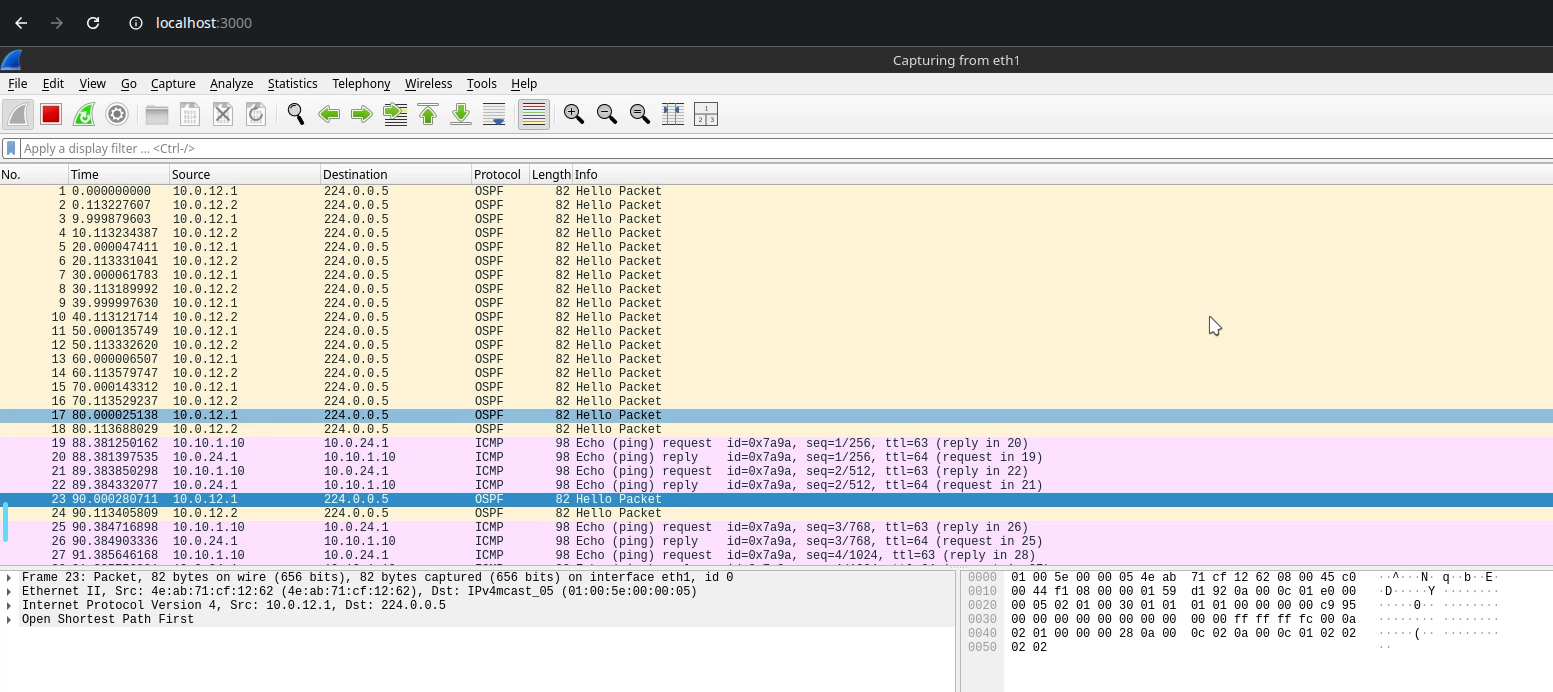
\includegraphics[width=0.92\textwidth,height=0.28\textheight,keepaspectratio]{images/wireshark_capture.png}
\caption{Runtime Wireshark capture on the \texttt{r1\_r2} collision domain of the generated multi-area laboratory.}
\label{fig:wireshark-runtime-capture}
\end{figure}

Figure~\ref{fig:wireshark-runtime-capture} provides a runtime check of the
monitoring integration. The generated Wireshark node is attached to the
selected collision domain and observes packets exchanged by the emulated nodes
without changing their functional roles. This complements inspection of
\texttt{lab.conf}: the generated file proves that the observation node was
configured, while the capture demonstrates that traffic on the selected
Kathar\'a segment is actually visible to it during execution.
}{}

The output of the generation stage is therefore a conventional Kathar\'a
laboratory enriched only by files that Kathar\'a already knows how to consume.
The framework's YAML format is used before generation; it is not required by
Kathar\'a at runtime. This design is significant because a generated laboratory
can be opened, inspected, and started with standard Kathar\'a tools even if the
generator is not invoked again.

\section{Laboratory Execution and Lifecycle Management}
\label{sec:laboratory-lifecycle}

Once generation is complete, the operational workflow returns to ordinary
Kathar\'a commands. The repository provides shell wrappers for the most common
lifecycle operations. Their purpose is intentionally limited: they perform
basic argument and directory checks, change into the selected laboratory, and
invoke the corresponding Kathar\'a command. Generation and runtime management
were deliberately not merged into one long-running Python process, because the
produced laboratory should remain usable even after the generator has exited.
The wrappers reduce repetitive shell navigation while keeping the underlying
Kathar\'a operation visible to the user.

Figure~\ref{fig:lifecycle-loop} presents the intended lifecycle. The YAML file
remains the source configuration. It is validated and generated into a
laboratory directory, which can then be started and inspected. When a persistent
change is required, the change is applied to the YAML source or to a node
resource directory and the laboratory is regenerated rather than relying on a
manual edit to derived output.

\begin{figure}[htbp]
\centering
\begin{tikzpicture}[
    node distance=12mm and 12mm,
    state/.style={draw, rounded corners, align=center, minimum width=2.6cm, minimum height=9mm, font=\small},
    arrow/.style={-{Latex[length=2mm]}, thick}
]
\node[state] (config) {Configure\\YAML source};
\node[state, right=of config] (validate) {Validate};
\node[state, right=of validate] (generate) {Generate\\laboratory};
\node[state, below=of generate] (start) {Start};
\node[state, left=of start] (inspect) {Inspect and\\verify};
\node[state, left=of inspect] (stop) {Stop};

\draw[arrow] (config) -- (validate);
\draw[arrow] (validate) -- (generate);
\draw[arrow] (generate) -- (start);
\draw[arrow] (start) -- (inspect);
\draw[arrow] (inspect) -- (stop);
\draw[arrow] (stop) -- node[pos=0.35,left,align=center]{modify source\\and regenerate}(config);
\end{tikzpicture}
\caption{Operational lifecycle of a generated laboratory.}
\label{fig:lifecycle-loop}
\end{figure}

A laboratory can be started with the wrapper by passing its generated path:

\begin{lstlisting}[language=bash,caption={Starting a generated laboratory.},label={lst:start-lab}]
./start.sh labs/client-router-server
\end{lstlisting}

The script requires at least one argument, derives the display name with
\texttt{basename}, verifies that the supplied directory exists, changes into
that directory, and executes:

\begin{lstlisting}[language=bash,caption={Kathar\'a command executed by start.sh.},label={lst:kathara-lstart}]
kathara lstart
\end{lstlisting}

Starting from the laboratory directory matters because Kathar\'a reads the
local \texttt{lab.conf} and the associated node files. During startup, the
collision-domain definitions in \texttt{lab.conf} determine the emulated links,
container images determine the node environments, and the \texttt{.startup}
files apply addresses, routes, FRRouting startup, and user commands. FRR-capable
nodes also find their configuration under their local
\texttt{/etc/frr/}-equivalent hostlab structure according to the standard
Kathar\'a file-mapping mechanism.

The wrapper is not required. The generator explicitly prints the equivalent
manual procedure after a successful run:

\begin{lstlisting}[language=bash,caption={Starting a laboratory without the wrapper.},label={lst:start-manual}]
cd labs/client-router-server
kathara lstart
\end{lstlisting}

Keeping both forms available is useful. The wrapper makes the common operation
shorter, while the explicit commands make it clear that the generated output is
not tied to the framework's own runtime.

After startup, individual nodes can be accessed through normal Kathar\'a
commands. For example:

\begin{lstlisting}[language=bash,caption={Connecting to a generated router.},label={lst:kathara-connect}]
kathara connect router
\end{lstlisting}

Once inside a node, standard Linux tools provide a first verification of the
generated configuration. \texttt{ip addr} shows whether addresses have been
assigned to the expected interface indices, \texttt{ip route} shows connected,
default, and static routes, and \texttt{ping} can be used for a basic
reachability check. In the minimal client-router-server topology, the client
can verify the path to the server address with:

\begin{lstlisting}[language=bash,caption={Basic reachability check after laboratory startup.},label={lst:basic-ping}]
ping 10.0.2.10
\end{lstlisting}

For FRRouting nodes, \texttt{vtysh} provides the corresponding routing view.
Commands such as \texttt{show ip route}, \texttt{show ip ospf neighbor}, and
\texttt{show ip bgp summary} are useful for verifying that the generated FRR
files have been loaded and that protocol state is developing as expected. These
manual checks are not part of generation itself. They are operational
observations performed after the generated files have been consumed by the
runtime environment.

This distinction is important because successful generation does not imply
immediate runtime convergence. The generator can prove that configured OSPF
networks refer to connected prefixes and that BGP neighbour declarations are
coherent according to the static model, but it cannot guarantee that a routing
protocol has converged at the exact moment the containers start. Runtime state
depends on process startup, neighbour availability, timers, imported resources,
and any user-supplied commands. Generation correctness and runtime behaviour
are therefore related but separate concerns.

The repository provides \texttt{stop.sh} for the inverse lifecycle operation:

\begin{lstlisting}[language=bash,caption={Stopping and cleaning the runtime environment.},label={lst:stop-lab}]
./stop.sh labs/client-router-server
\end{lstlisting}

Like \texttt{start.sh}, the script verifies that the supplied directory exists
and changes into it. It then invokes the standard Kathar\'a cleanup command
\cite{kathara_manpage}:

\begin{lstlisting}[language=bash,caption={Kathar\'a command executed by stop.sh.},label={lst:kathara-lclean}]
kathara lclean
\end{lstlisting}

The word \emph{clean} in this Kathar\'a command should not be confused with the
generator's \cliopt{clean} option. \texttt{kathara lclean} removes the
runtime laboratory created by Kathar\'a, including the containers and associated
runtime networking, while the generated directory on disk remains available.
The generator's \cliopt{clean}, by contrast, operates on the file-system
output before generation: it deletes the selected laboratory directory and
recreates its files from the YAML source.

The difference can be summarised as follows:

\begin{table}[htbp]
\centering
\small
\begin{tabular}{p{0.25\textwidth}p{0.31\textwidth}p{0.30\textwidth}}
\toprule
\textbf{Operation} & \textbf{Generated files} & \textbf{Runtime containers and networks} \\
\midrule
Generation & Created or overwritten & Not started by the generator \\
\texttt{start.sh} / \texttt{kathara lstart} & Preserved & Created and started \\
\texttt{stop.sh} / \texttt{kathara lclean} & Preserved & Removed \\
Generation with \cliopt{clean} & Directory removed and regenerated & Independent of runtime state \\
\texttt{del\_lab.sh} & Selected generated directory removed & Does not replace runtime cleanup \\
\bottomrule
\end{tabular}
\caption{Effects of the main lifecycle operations.}
\label{tab:lifecycle-effects}
\end{table}

When the generated files are no longer required, \texttt{del\_lab.sh} removes
them from disk. It accepts either a path to a laboratory directory or the
literal argument \texttt{all}. For an individual laboratory:

\begin{lstlisting}[language=bash,caption={Deleting one generated laboratory.},label={lst:delete-one-lab}]
./del_lab.sh labs/client-router-server
\end{lstlisting}

and for all generated content under \texttt{labs/}:

\begin{lstlisting}[language=bash,caption={Deleting all generated laboratories.},label={lst:delete-all-labs}]
./del_lab.sh all
\end{lstlisting}

The current implementation performs deletion with \texttt{sudo rm -rf}. When
\texttt{all} is supplied, only the contents of \texttt{./labs/} are removed and
the parent directory itself is preserved. For a specific argument, the script
first checks that the path exists as a directory and then removes that path.
Because this is a destructive file-system operation, the selected path should
be verified before invoking the command. In normal use, runtime cleanup with
\texttt{stop.sh} should be treated separately from removal of generated files.

The explicit path accepted by the lifecycle scripts also allows several
laboratories to coexist under the same output directory. A repository may, for
example, contain:

\begin{lstlisting}[caption={Several generated laboratories coexisting under labs/.},label={lst:multiple-labs}]
labs/
|-- client-router-server/
|-- Test1_multi_area/
|-- multi-AS/
`-- Test_enterprise_multi_as_import_dirs/
\end{lstlisting}

No lifecycle script needs to guess which one is active or intended. This
explicit selection also reflects a development issue that appeared as the
number of example configurations increased: assumptions that were harmless
when only one generated laboratory was present became ambiguous once several
outputs coexisted under \texttt{labs/}. The user therefore selects the
laboratory explicitly:

\begin{lstlisting}[language=bash,caption={Starting one laboratory among several generated environments.},label={lst:start-specific-lab}]
./start.sh labs/multi-AS
\end{lstlisting}

This explicit selection is consistent with the framework's general design: the
tool automates repetitive file creation and common commands, but avoids hidden
choices when more than one valid target exists.

The lifecycle also clarifies which artefact should be considered authoritative.
The YAML configuration is the source description, while the directory under
\texttt{labs/} is derived output. A persistent topology change should therefore
be applied to the YAML source. A persistent node-resource change should be
applied to the resource directory located next to that YAML file. After the
change, the laboratory can be regenerated, preferably with \cliopt{clean}
when a fully reconstructed output is required.

Directly editing \texttt{lab.conf}, a generated startup file, or a generated
FRR file is possible because they are ordinary text files, but such edits are
not part of the reproducible source model. A later clean generation replaces
them. Treating generated files as disposable output reduces configuration drift
between the declarative source and the laboratory that is actually executed.
The relationship can be expressed as:

\begin{lstlisting}[caption={Source and derived-output relationship.},label={lst:source-output}]
configs/<topology>.yml       -> authoritative topology source
configs/<node>/             -> authoritative optional node resources

labs/<lab-name>/            -> generated laboratory output
\end{lstlisting}

There are several practical boundaries to this workflow. Docker and Kathar\'a
must already be installed and correctly configured for the current user; the
generator does not provision those dependencies. The selected container images
must also provide the commands expected by the generated startup files. Forced
generation can leave obsolete files in an existing directory, whereas clean
generation intentionally removes manual changes made to the output. Imported
resources depend on the naming convention that associates a source directory
with a YAML node of the same name. Advanced Linux behaviour outside the
configuration model must be supplied through startup commands, and advanced
FRRouting behaviour can be supplied through manual FRR content, which reduces
the amount of semantic checking the framework can perform.

A further implementation detail concerns FRR-capable node roles. Because
\texttt{router}, \texttt{switch}, and \texttt{firewall} are recognised as FRR
devices by type, those nodes receive FRR startup and configuration files even
when the configuration does not select OSPF, RIP, or BGP. In that case the
framework writes a minimal \texttt{frr.conf} containing the hostname,
integrated VTY configuration, and a VTY section, while protocol daemons remain
disabled. This keeps the behaviour predictable for routing-oriented images,
but it also means that node type influences generated runtime configuration in
addition to documenting the conceptual role of the node.

These boundaries do not change the central lifecycle model. The framework takes
responsibility for deterministic transformations it can express explicitly,
then hands a normal Kathar\'a laboratory to the standard runtime. This makes the
generated output inspectable and reduces the amount of project-specific logic
required once generation has finished.

\section{Chapter Summary}
\label{sec:laboratory-generation-summary}

This chapter described how the validated configuration model is transformed
into an executable Kathar\'a laboratory. The command-line wrapper delegates the
process to \texttt{src\_gen\_lab.gen\_lab}, which validates the input, prepares
the output directory, creates \texttt{lab.conf}, writes node startup files,
generates FRRouting configuration for FRR-capable devices, and optionally
imports node-specific resources or adds a Wireshark observation node.

The generated artefacts preserve the standard Kathar\'a structure. Collision
domains and image assignments are written to \texttt{lab.conf}; addresses,
default gateways, static routes, FRR startup, and custom commands are written
to per-node startup files; and routing devices receive the appropriate
\texttt{daemons}, \texttt{frr.conf}, and \texttt{vtysh.conf} files. The same
validated YAML information can therefore influence several output files without
requiring the user to duplicate the configuration manually.

After generation, the framework does not replace the Kathar\'a runtime.
\texttt{start.sh} and \texttt{stop.sh} are thin wrappers around
\texttt{kathara lstart} and \texttt{kathara lclean}, while
\texttt{del\_lab.sh} manages the generated directories on disk. Nodes remain
accessible through standard Kathar\'a commands and can be inspected with Linux
networking tools and FRRouting's \texttt{vtysh}. Multiple generated laboratories
can coexist because lifecycle operations receive an explicit laboratory path.

Most importantly, the YAML configuration remains the authoritative description
of the topology and the generated laboratory remains derived output. This
separation supports reproducibility: changes are made at the source level and
propagated through validation and regeneration, while the generated files stay
compatible with the ordinary Kathar\'a workflow.


\chapter{Experimental Evaluation and Controlled DoS Experiment}
\label{chap:experimental-evaluation}

The previous chapters described the framework as a software system: the input
model, the validation rules, the generation of Kathar\'a artefacts, and the
lifecycle used to start and inspect a generated laboratory. This chapter moves
from implementation to experimental use. Its purpose is to verify that the
framework can support a repeatable network experiment in which several
legitimate hosts access the same service concurrently and their observations
are collected before and during a controlled adverse workload.

The experiment is intentionally bounded and is executed entirely inside the
local Kathar\'a environment. No traffic is directed towards external systems.
The adverse workload is therefore used as an experimental condition rather
than as a general-purpose attack mechanism. The objective is to observe how a
finite-capacity TCP application behaves when many connections compete for its
available service slots, and to determine whether client-side and server-side
measurements can describe that transition quantitatively.

\noindent\textbf{Real-world DDoS context.}
The controlled experiment should be interpreted against the broader evolution
of Distributed Denial-of-Service attacks. Real incidents can exhaust different
resources and can rely on compromised botnets, reflection and amplification,
protocol-specific techniques, or application-layer request floods
\cite{rfc4732}. The laboratory developed in this thesis does not attempt to
reproduce the scale, source diversity, or attack infrastructure of such
incidents. Instead, selected cases are useful because they identify several
distinct mechanisms that a small emulated experiment can abstract only in
part.

\begin{table}[htbp]
\centering
\small
\begin{tabular}{p{0.18\textwidth}p{0.32\textwidth}p{0.38\textwidth}}
\toprule
\textbf{Incident} & \textbf{Main characteristic} & \textbf{Relation to this thesis} \\
\midrule
Mirai / Dyn, 2016 &
A Mirai-variant botnet composed of compromised Internet-of-Things devices was
used in DDoS activity that impacted Dyn's DNS infrastructure and disrupted
access to multiple major Internet services \cite{doj_mirai_dyn_2020}. &
This is the closest structural analogy to the controller and multiple load
agents used in the Kathar\'a testbed: several distributed sources converge on
a common service. The laboratory agents, however, are deliberately controlled,
bounded, and non-compromised. \\

GitHub, 2018 &
A memcached UDP reflection/amplification attack reached a peak of
1.35~Tbps and 126.9 million packets per second
\cite{github_ddos_2018}. &
This case illustrates a mechanism that is intentionally not reproduced by the
framework. The attack relied on reflectors, source-address spoofing, and
amplification rather than on direct TCP connection generators. \\

Google HTTP/2 Rapid Reset, 2023 &
A Layer~7 campaign using the HTTP/2 Rapid Reset technique reached a peak of
398 million requests per second. The underlying issue was tracked as
CVE-2023-44487 \cite{google_rapid_reset_2023}. &
The event shows that DDoS intensity cannot be described only in bit/s. Request
rate and server or proxy processing capacity may also become the limiting
resource, which is conceptually closer to the finite application capacity
studied in this chapter. \\

Cloudflare, 2025 &
Cloudflare reported blocking a 7.3~Tbps multi-vector DDoS attack that delivered
37.4~TB in 45 seconds; approximately 99.996\% of the traffic was classified as
UDP floods \cite{cloudflare_ddos_2025}. &
This case illustrates the modern hyper-volumetric and short-duration extreme.
The present experiment deliberately studies a different question: the
relationship between offered workload and available service capacity, rather
than Internet-scale throughput. \\
\bottomrule
\end{tabular}
\caption{Selected real-world DDoS incidents used to contextualise the controlled experiment.}
\label{tab:real-world-ddos-cases}
\end{table}

DDoS is also used outside purely criminal or commercial contexts. Europol's
2026 Internet Organised Crime Threat Assessment describes the pro-Russian
NoName057(16) network as a prominent example of ideologically motivated DDoS
activity. In July 2025, Operation Eastwood disrupted more than 100 servers
associated with the infrastructure; Europol linked the network to an average
of 73 DDoS attacks per day against Ukrainian public and private actors and
reported that activity resumed after an initial decline
\cite{europol_iocta_2026}. This example is relevant because it shows that the
availability objective of a DDoS attack can remain similar even when the
operational motivation and infrastructure are very different.

These cases define an important boundary for the evaluation. The experiment
does not claim to reproduce an Internet-scale botnet, reflection/amplification,
HTTP/2 protocol exploitation, or multi-terabit flooding. Because several
controlled agents contribute simultaneously, the workload has a
distributed-source structure, but the term \emph{controlled DoS} is retained
to emphasise the deliberately bounded laboratory scope. What the experiment
does reproduce is a narrower and measurable resource-contention mechanism:
multiple sources compete with legitimate clients for finite service capacity.
Consequently, the most relevant variables are not absolute traffic volume but
application completion, lower-layer reachability, response time, and the
server-side capacity state. Sections~\ref{sec:measurement-baseline} and
\ref{sec:controlled-dos-results} measure these variables directly.

The archived project contains five complete repetitions for each topology,
collected on 13 October 2026 with the same eight clients, ten concurrent
measurement rounds, and controlled workload schedule. The direct-server runs
are stored under \path{results/dos_lab/simulation_0001/} through
\path{simulation_0005/}; the five complete reverse-proxy runs are stored under
\path{results/mitigation/simulation_0002/} through
\path{simulation_0006/}. Each run contains a baseline and a controlled-load
phase, and every phase file contains 80 client observations. The resulting
dataset therefore comprises 1,600 client observations: 800 per topology and,
within each topology, 400 for the baseline and 400 for the controlled-load
phase. The final dataset was defined as executions containing both client-phase
CSV files with 80 observations per phase together with the server-side metric
files; no observation from a run satisfying this completeness criterion was
excluded. The directory \path{results/mitigation/simulation_0001/} is a
preliminary pilot collected before the routing-readiness criterion was added.
It contains server metrics but no client-result CSV and was therefore never a
member of the final dataset. The first complete run of each topology is
retained below as a detailed representative execution;
Section~\ref{sec:repeated-run-validation} then treats the ten complete runs as
the descriptive dataset. All numerical results were recalculated directly from
the archived CSV files rather than transcribed from console output.

\section{Experimental Methodology and Testbed}
\label{sec:experimental-methodology}

The experimental testbed is generated from \path{configs/dos_lab.yml}. It is a
multi-LAN enterprise-style topology composed of two legitimate-user networks,
a routed core, a separate network containing the controlled load agents, and a
DMZ containing the application server. All routers use OSPF in area 0, so the
experiment also depends on the routing configuration produced by the framework
rather than on a single flat collision domain.

The two legitimate LANs contain four hosts each. The first LAN uses the
prefix \texttt{10.10.1.0/24} and contains \texttt{pc\_a1} through
\texttt{pc\_a4}; the second uses \texttt{10.10.2.0/24} and contains
\texttt{pc\_b1} through \texttt{pc\_b4}. The target service is hosted by
\texttt{server} at \texttt{10.30.1.10/24} in the DMZ. A separate workload
network uses \texttt{10.20.1.0/24} and contains the controller
\texttt{attacker} together with three bounded load agents,
\texttt{zombie\_1}, \texttt{zombie\_2}, and \texttt{zombie\_3}. The
corresponding collision-domain names are reported in the configuration and the
functional roles are summarised in Table~\ref{tab:experimental-nodes}.

\begin{table}[htbp]
\centering
\small
\begin{tabular}{p{0.24\textwidth}p{0.28\textwidth}p{0.36\textwidth}}
\toprule
\textbf{Component} & \textbf{Nodes / address range} & \textbf{Role} \\
\midrule
Legitimate LAN A & \texttt{pc\_a1}--\texttt{pc\_a4}, \texttt{10.10.1.0/24} & Concurrent legitimate clients connected through \texttt{r1}. \\
Legitimate LAN B & \texttt{pc\_b1}--\texttt{pc\_b4}, \texttt{10.10.2.0/24} & Concurrent legitimate clients connected through \texttt{r2}. \\
Routing core & \texttt{r1}, \texttt{r2}, \texttt{r3}, \texttt{r4}, \texttt{core} & OSPF infrastructure connecting the client LANs, the DMZ, and the isolated workload LAN. \\
Service DMZ & \texttt{server}, \texttt{10.30.1.10/24} & Instrumented TCP application exposed on port \texttt{9000}. \\
Controlled-load LAN & \texttt{attacker}, \texttt{zombie\_1}--\texttt{zombie\_3}, \texttt{10.20.1.0/24} & Controller and bounded connection generators used only inside the laboratory. \\
\bottomrule
\end{tabular}
\caption{Main components of the experimental topology.}
\label{tab:experimental-nodes}
\end{table}

Figure~\ref{fig:dos-testbed} shows the logical structure of the testbed. The
central point is that legitimate traffic and controlled workload traffic reach
the same server through the routed infrastructure. This makes the experiment a
test not only of the application but also of the complete laboratory generated
by the framework: addressing, gateways, inter-router links, OSPF routes, node
resources, and service startup commands all have to operate consistently.

\begin{figure}[htbp]
\centering
\resizebox{0.94\textwidth}{!}{%
\begin{tikzpicture}[
    node distance=10mm and 14mm,
    host/.style={draw, rounded corners, align=center, minimum width=2.3cm, minimum height=8mm},
    router/.style={draw, diamond, aspect=2.1, align=center, inner sep=1.2pt},
    net/.style={draw, dashed, rounded corners, align=center, minimum width=2.6cm, minimum height=8mm},
    line/.style={thick}
]
\node[host] (lana) {4 clients\\LAN A};
\node[router, right=of lana] (r1) {r1};
\node[router, right=18mm of r1] (r3) {r3};
\node[router, below=15mm of r1] (r2) {r2};
\node[router, right=18mm of r2] (r4) {r4};
\node[router, right=18mm of r3, yshift=-10mm] (core) {core};
\node[host, left=of r2] (lanb) {4 clients\\LAN B};
\node[host, right=20mm of core, yshift=11mm] (server) {server\\10.30.1.10};
\node[host, right=20mm of core, yshift=-14mm] (load) {attacker +\\3 agents};

\draw[line] (lana) -- node[above]{\scriptsize \texttt{lan\_a}} (r1);
\draw[line] (lanb) -- node[below]{\scriptsize \texttt{lan\_b}} (r2);
\draw[line] (r1) -- (r2);
\draw[line] (r1) -- (r3);
\draw[line] (r2) -- (r4);
\draw[line] (r3) -- (r4);
\draw[line] (r2) -- (core);
\draw[line] (r3) -- (core);
\draw[line] (r4) -- (core);
\draw[line] (core) -- node[above,sloped]{\scriptsize DMZ} (server);
\draw[line] (core) -- node[below,sloped]{\scriptsize workload LAN} (load);
\end{tikzpicture}%
}
\caption{Logical structure of the controlled experimental testbed.}
\label{fig:dos-testbed}
\end{figure}

The experiment is orchestrated by \path{simulate.sh}. By default the script
selects \texttt{dos\_lab}, targets the node named \texttt{server} on TCP port
\texttt{9000}, discovers all nodes whose names begin with \texttt{pc\_} as
legitimate clients, and creates a new numbered output directory under
\path{results/dos_lab/}. Earlier connectivity utilities were more dependent on
literal addresses; accepting a logical target name where possible reduced the
need to repeat addressing information already represented by the laboratory
configuration and made the same test workflow easier to reuse after address
changes. A full run first performs the baseline measurement and then performs
the controlled-load measurement using the same laboratory and the same
measurement parameters.

The default parameters used by all archived complete runs are ten
simultaneous rounds, a three-second measurement timeout, one second between
rounds, and a 25-second startup wait when the orchestrator starts the lab. The
script also checks reachability of the target from every legitimate client
before starting the measurements. This routing-readiness stage repeatedly sends
an ICMP probe from each client and allows up to 120 seconds for the routes to
become usable. The check was introduced after earlier executions showed that a
measurement could start while dynamic routing was not yet usable from every
client. A fixed startup delay alone was therefore not considered a sufficient
readiness criterion. By checking the observed network state, an OSPF
convergence problem can be detected before it contaminates the service
baseline. This is particularly relevant in light of the preliminary
\path{mitigation/simulation_0001} pilot described above: because it predates
this criterion and contains no client-result dataset, it is retained only as a
development artefact and is not analysed as an experimental run.

Table~\ref{tab:experimental-environment} records the software and host
environment used for the archived experiments. These values were captured on
the experimental host when the results were archived on 13 October 2026. The
Git working tree contained uncommitted changes, so the base commit alone is not
a byte-for-byte identifier of the executed source; the archived project files,
configuration files, raw CSV data, and container-image digests are therefore
the authoritative experimental artefacts.

\begin{table}[htbp]
\centering
\small
\begin{tabular}{p{0.28\textwidth}p{0.62\textwidth}}
\toprule
\textbf{Component} & \textbf{Recorded value} \\
\midrule
Host processor & 11th Gen Intel Core i7-11800H at 2.30 GHz; 16 logical CPUs \\
Host memory & 15 GiB RAM; 2 GiB swap \\
Operating system & Linux Mint 22.2; Linux kernel \texttt{7.0.0-34-generic} \\
Python / PyYAML & Python 3.12.3; PyYAML 6.0.1 \\
Docker & Client and server 29.8.1 \\
Kathar\'a & Version 3.8.3 \\
\texttt{kathara/base:latest} &
\texttt{sha256:8a2e70ac8f51bb283b8549fd686f65f9}\allowbreak
\texttt{a1ef4487fe2c81849cb74d301e61970b} \\
\texttt{kathara/frr:latest} &
\texttt{sha256:3b7a3f630d8ecd9efddd4586ba2f0a41}\allowbreak
\texttt{e2c462f13bc81dee8e3c6ebac183f57c} \\
Framework source & Git base commit \texttt{3a1d65189981}; working tree dirty \\
\bottomrule
\end{tabular}
\caption{Host, software, and container-image metadata recorded for the
experimental archive.}
\label{tab:experimental-environment}
\end{table}

The results of each run are isolated by a run number. Client
measurements are separated by scenario in
\path{connection_results_baseline.csv} and
\path{connection_results_dos.csv}; service-side counters are stored in
\path{server_metrics.csv}; and host-level Docker samples are stored in
\path{server_container_metrics.csv}. The same run identifier is also
used by the logging hierarchy, which makes it possible to associate a client
failure with the corresponding server state and orchestration run. The
mitigation runs retain the same schema: the \texttt{target\_input} field changes
from \texttt{server} to \texttt{proxy}, while the public address and port remain
\texttt{10.30.1.10:9000}.

\section{Measurement Infrastructure and Baseline Evaluation}
\label{sec:measurement-baseline}

The target application is implemented by \path{configs/server/service.py}. It
is a multithreaded TCP service that listens on port \texttt{9000}. A bounded
semaphore, implemented with
\texttt{threading.}\allowbreak\texttt{BoundedSemaphore}, limits the number of
active application sessions. In the experimental YAML and in the orchestration
fallback command, \texttt{SERVICE\_MAX\_ACTIVE} is set to 20 and
\texttt{SERVICE\_BACKLOG} is set to 20. A connection that cannot acquire an
application slot is answered with \texttt{BUSY} when possible and then closed.
A connection that obtains a slot receives a small text menu; selection
\texttt{1} returns the token \texttt{pong}.

This behaviour allows the experiment to distinguish network reachability, TCP
connectivity, and application availability. This distinction grew out of a
concrete development problem: a client could reach the server node while the
application process was not running or was unable to complete the expected
transaction. Treating reachability as a successful service test therefore
produced misleading results. A successful ICMP reply proves only that the
routed path is currently reachable, while a successful TCP handshake proves
that the kernel accepted a connection to the server port. Neither event alone
proves that the application completed the requested operation. For this reason,
\path{run_connection_tests.py} treats a request as successful only when the
client sends \texttt{1} and subsequently observes \texttt{pong} in the server
response.

Each measurement is executed inside the client container rather than on the
Docker host. The script records five timing fields, listed in
Table~\ref{tab:measurement-metrics}. This separation is important because the
host-side time required to invoke \texttt{docker exec} is not a network delay
and should not be interpreted as one.

\begin{table}[htbp]
\centering
\small
\begin{tabular}{p{0.31\textwidth}p{0.57\textwidth}}
\toprule
\textbf{Metric} & \textbf{Meaning} \\
\midrule
\texttt{icmp\_rtt\_ms} & Round-trip time of a single ICMP echo request executed in the client network namespace. \\
\texttt{tcp\_connect\_ms} & Time from the beginning of \texttt{connect()} to successful establishment of the TCP connection. \\
\texttt{application\_response\_ms} & Time between sending selection \texttt{1} and receiving a response containing \texttt{pong}. \\
\texttt{request\_completion\_ms} & Complete TCP application transaction from the start of connection establishment to reception of \texttt{pong}. \\
\path{host_command_completion_ms} & Host-observed duration of the complete measurement command, including Docker invocation overhead. \\
\bottomrule
\end{tabular}
\caption{Client-side metrics recorded by \texttt{run\_connection\_tests.py}.}
\label{tab:measurement-metrics}
\end{table}

The execution model was also changed during development. A sequential strategy
is sufficient when the question is simply whether each client can reach a
service, but it becomes problematic when clients are intended to observe a
shared and time-varying server condition. Executing all attempts from one host
before moving to the next would compare measurements collected in different
windows and could make an overload transition appear different for each client.
For every request index, the final implementation therefore schedules the eight
legitimate clients concurrently through a \texttt{ThreadPoolExecutor}. The
execution model is round based rather than client based: in round~1 all eight
clients perform one measurement; after the configured delay, round~2 repeats
the same operation, and so on. With eight clients and ten attempts, each
scenario produces 80 application requests. Concurrency is therefore an
experimental requirement for comparability, not merely a performance
optimisation.

Application availability is defined as

\begin{equation}
A = \frac{N_{\mathrm{pong}}}{N_{\mathrm{requests}}} \times 100,
\label{eq:application-availability}
\end{equation}

where $N_{\mathrm{pong}}$ is the number of requests for which the expected
application response was received. Failed requests remain part of the
denominator. Latency summaries, on the other hand, can only be calculated from
requests for which the corresponding timing value exists. This distinction is
essential under overload: a low mean response time among the small subset of
successful requests does not imply a healthy service when most requests fail.

As a representative execution, the baseline of
\path{dos_lab/simulation_0001} contains 80 requests and all 80
completed successfully, corresponding to 100\% application availability. All
ICMP probes and all TCP connection attempts were also successful. The mean
ICMP RTT was 1.686 ms and the mean TCP connection time was 1.803 ms. Among the
successful application requests, the mean response time was 3.218 ms, the
median was 3.202 ms, the 95th percentile was 4.922 ms, and the maximum was
5.309 ms. Table~\ref{tab:baseline-summary} reports the main values.

\begin{table}[htbp]
\centering
\small
\begin{tabular}{lr}
\toprule
\textbf{Baseline metric} & \textbf{Value} \\
\midrule
Legitimate application requests & 80 \\
Successful application requests & 80 \\
Application availability & 100.00\% \\
ICMP successes & 80 / 80 \\
TCP connection successes & 80 / 80 \\
Mean ICMP RTT & 1.686 ms \\
Mean TCP connection time & 1.803 ms \\
Mean application response time & 3.218 ms \\
Median application response time & 3.202 ms \\
95th percentile application response time & 4.922 ms \\
Maximum application response time & 5.309 ms \\
Approximate measurement duration & 10.77 s \\
\bottomrule
\end{tabular}
\caption{Direct-server baseline results from \texttt{dos\_lab/simulation\_0001}.}
\label{tab:baseline-summary}
\end{table}

Figure~\ref{fig:direct-baseline-metrics} reports the corresponding per-client
measurements. The availability panel remains at 100\% in every round, while the
other panels show the short-timescale variation in ICMP, TCP, and application
response times summarised in Table~\ref{tab:baseline-summary}.

\begin{figure}[p]
\centering
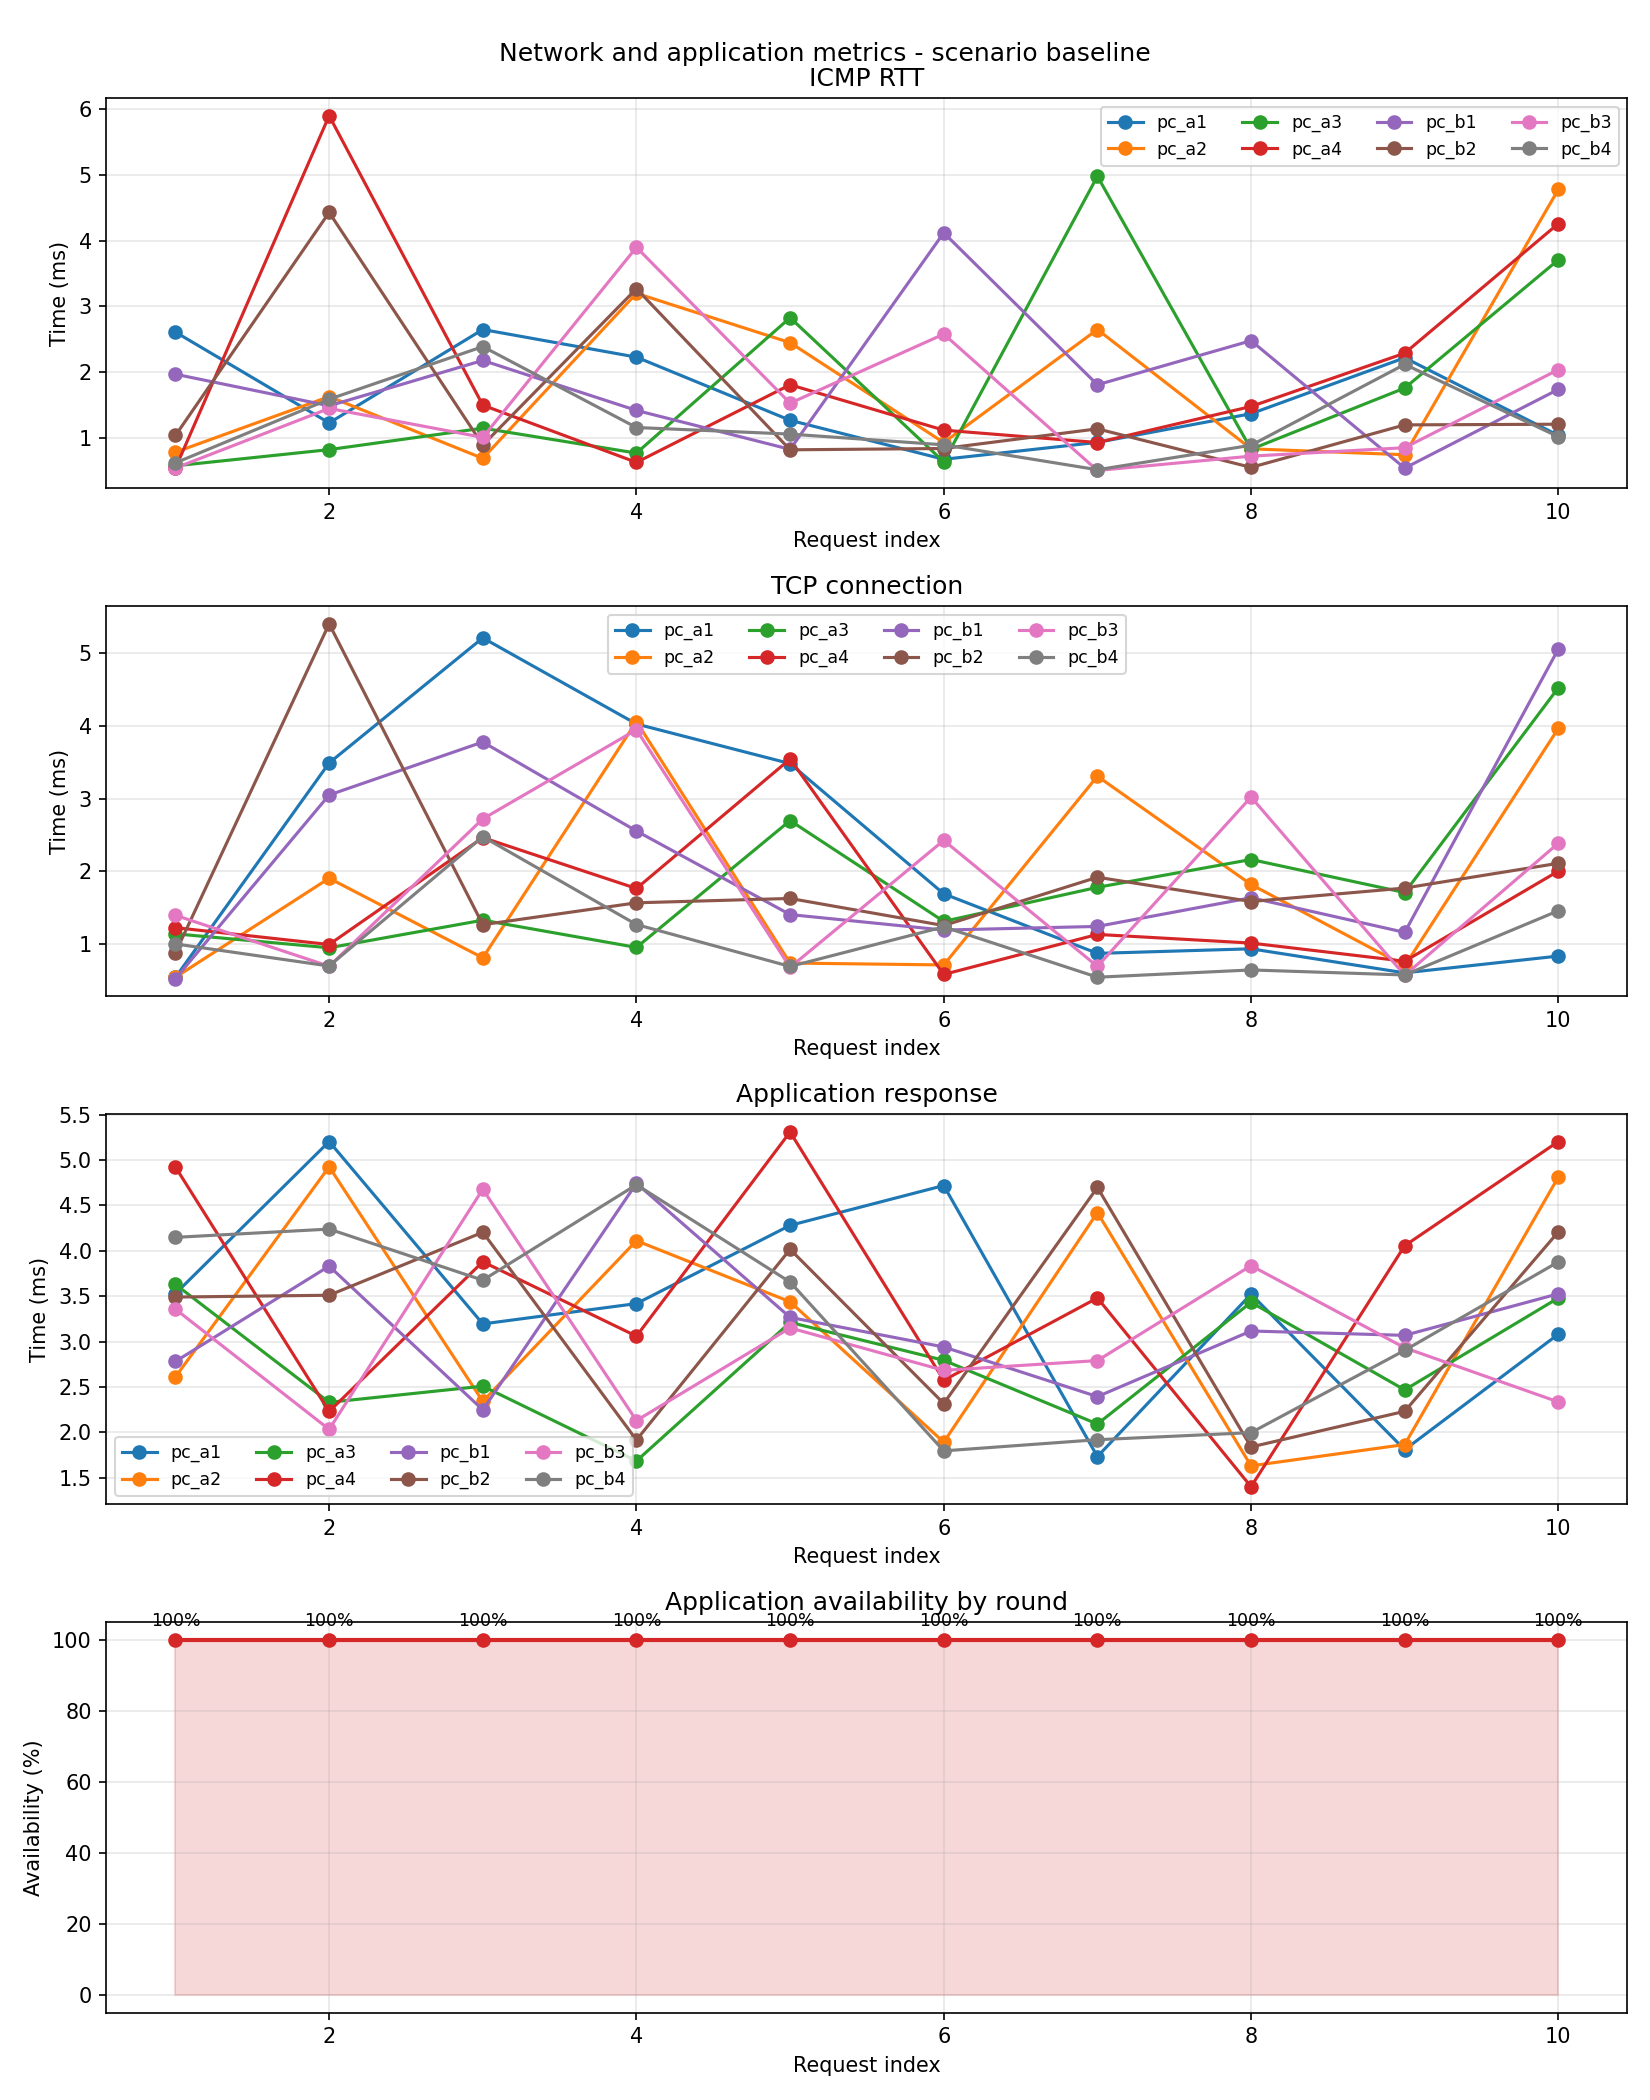
\includegraphics[width=0.90\textwidth]{images/dos_lab_simulation_0001_baseline_metrics.png}
\caption{Per-client network and application measurements for the direct-server baseline in \texttt{dos\_lab/simulation\_0001}.}
\label{fig:direct-baseline-metrics}
\end{figure}

The per-client baseline is also uniform. Every client completed ten out of ten
requests successfully. No client exhibits an availability disadvantage. This
is relevant because the clients are attached
to two different access LANs and traverse different first-hop routers; the
baseline therefore establishes that the generated routing topology does not
itself introduce a visible service failure before the adverse workload is
introduced.

The server-side metrics reinforce the same conclusion. During the baseline
window, the instrumented service recorded 80 accepted connection events and no
\texttt{BUSY} or rejected events. The maximum number of simultaneously active
connections observed by the server was one and the maximum active thread count
was four. The container sampler collected six Docker-stat samples for the
baseline window; these samples reported a mean CPU utilisation of approximately
0.53\% and a maximum of 0.88\%. Since the baseline measurement lasts only about
ten seconds and the container dataset contains a small number of samples, these
resource figures are used descriptively rather than as statistically stable
estimates of host consumption.

The mitigation baseline in \path{mitigation/simulation_0002} independently
satisfies the same validity criteria: all eight clients are present in every
round, all 80 ICMP and TCP checks succeed, and all 80 application transactions
complete. Its application response is slower because the transaction traverses
the proxy: the mean is 6.058 ms, compared with 3.218 ms for the direct-server
baseline. This baseline cost is considered together with the protection result
in Section~\ref{sec:mitigation-results}.

\section{Controlled DoS Experiment and Observed Results}
\label{sec:controlled-dos-results}

The controlled DoS phase was not part of the initial topology-generation
requirement. It was introduced only after generation, routing, and service
measurement were sufficiently stable to support a controlled comparison between
two operating conditions. Reusing the same topology and measurement path was
preferred to building a separate attack-specific environment, because it keeps
the baseline and adverse phases comparable and turns the experiment into an
extension of the existing verification workflow.

The second phase introduces a bounded connection-based workload while the same
eight legitimate clients continue to use the same application interface. The
experiment is best interpreted as connection-capacity contention rather than as
a bandwidth-flooding benchmark. Each controlled agent opens several TCP
connections to the service and attempts to keep them established for a bounded
period. The target application, by contrast, exposes only 20 concurrent
application slots. The expected effect is therefore contention for finite
server-side session capacity, not saturation of a physical link.

The control architecture consists of one \texttt{attacker} node and three
agents. Each agent listens on TCP port \texttt{9999}. The controller reads the
agent addresses from \path{zombies.txt} and sends a command containing the
target address, target port, requested number of connections, and duration. The
orchestrator uses 40 requested connections per agent and a 60-second duration
by default, with an additional global cap that prevents a configured duration
above 90 seconds. With three agents, the requested workload therefore consists
of up to 120 concurrent connection workers competing with a service configured
for 20 active application sessions.

The agents are themselves bounded. The implementation limits the number of
connections created by one agent and limits the duration of a load episode.
Each worker reconnects when necessary so that pressure can be maintained across
the configured interval even if a server-side timeout closes an idle
connection. These restrictions make the mechanism suitable for a repeatable
laboratory experiment: load intensity and duration are explicit parameters and
the agent remains confined to the addresses provided by the controller inside
the generated topology.

The full orchestration does not simply start the workload and then begin
measuring. Client measurement starts first, while workload activation is
scheduled asynchronously after the configured start delay. In the direct-server
run this creates a visible transition within the same result file. The
first two request rounds complete successfully for all eight legitimate
clients; from round 3 onward, none of the legitimate requests receives a valid
\texttt{pong}. Table~\ref{tab:availability-rounds} shows this progression.

\begin{table}[htbp]
\centering
\small
\begin{tabular}{cccc}
\toprule
\textbf{Round} & \textbf{Requests} & \textbf{Successful} & \textbf{Availability} \\
\midrule
1 & 8 & 8 & 100\% \\
2 & 8 & 8 & 100\% \\
3 & 8 & 0 & 0\% \\
4 & 8 & 0 & 0\% \\
5 & 8 & 0 & 0\% \\
6 & 8 & 0 & 0\% \\
7 & 8 & 0 & 0\% \\
8 & 8 & 0 & 0\% \\
9 & 8 & 0 & 0\% \\
10 & 8 & 0 & 0\% \\
\bottomrule
\end{tabular}
\caption{Application availability by request round during the direct-server controlled-load measurement.}
\label{tab:availability-rounds}
\end{table}

Across the complete controlled-load measurement, 16 of 80 legitimate requests
succeeded, giving an overall availability of 20\%. This percentage includes the
first two rounds, which completed before the controlled workload became active.
During the attack-active interval, from rounds 3 through 10, none of the 64
legitimate application requests completed successfully; application
availability while the workload was active was therefore 0\%. The 20\% value
must consequently be interpreted as the availability of the complete transition
run, whereas 0\% describes the period in which the adverse workload was
actually active. Importantly, all 80 ICMP probes succeeded and all 80 TCP
handshakes were recorded as successful. Of the 64 application failures, 47 did
not receive the expected \texttt{pong} and 17 reported a connection reset as
\texttt{socket\_error:104} after the TCP connection had already been
established. The experiment therefore exhibits a
clear separation between network-level reachability and application-level
availability.

This result is one of the central observations of the evaluation. If the test
had relied on \texttt{ping} alone, the service would have appeared fully
reachable during the entire workload window. If it had relied only on TCP
connection establishment, the same conclusion would have been reached, because
all handshakes succeeded. Only the application-level request identifies that 64
of the 80 legitimate transactions did not complete successfully. In other
words, a reachable host and an open TCP port do not imply that the service is
currently able to satisfy legitimate work.

The timing values show the same distinction. Mean ICMP RTT increased from
1.686 ms in the baseline to 2.127 ms during the controlled-load run. Mean TCP
connection time increased from 1.803 ms to 2.198 ms. Among the 16 requests that
still succeeded, mean application response time was 3.432 ms, the median was
3.347 ms, the 95th percentile was 4.567 ms, and the maximum was 4.735 ms.
These successful-request
latencies alone would suggest only modest change. The major degradation is
therefore represented by the fall in completion probability, not by a large
increase in the latency of transactions that happen to complete.

\begin{table}[htbp]
\centering
\small
\begin{tabular}{lrr}
\toprule
\textbf{Metric} & \textbf{Baseline} & \textbf{Controlled run} \\
\midrule
Legitimate requests & 80 & 80 \\
Successful application requests & 80 & 16 \\
Overall application availability & 100.00\% & 20.00\% \\
Attack-active application availability & -- & 0.00\% \\
Successful ICMP probes & 80 & 80 \\
Successful TCP handshakes & 80 & 80 \\
Mean ICMP RTT & 1.686 ms & 2.127 ms \\
Mean TCP connection time & 1.803 ms & 2.198 ms \\
Mean application response time$^{*}$ & 3.218 ms & 3.432 ms \\
Median application response time$^{*}$ & 3.202 ms & 3.347 ms \\
95th percentile application response$^{*}$ & 4.922 ms & 4.567 ms \\
Maximum application response time$^{*}$ & 5.309 ms & 4.735 ms \\
\bottomrule
\end{tabular}
\caption{Client-side comparison for \texttt{dos\_lab/simulation\_0001}. Values marked with $^{*}$ are calculated only from requests that produced an application response.}
\label{tab:client-comparison}
\end{table}

The transition is visible directly in
Figure~\ref{fig:direct-dos-metrics}: application availability is 100\% in the
first two rounds and falls to 0\% from round 3 onward. Application-response
curves consequently stop after round 2, although the ICMP and TCP panels retain
measurements for all ten rounds.

\begin{figure}[p]
\centering
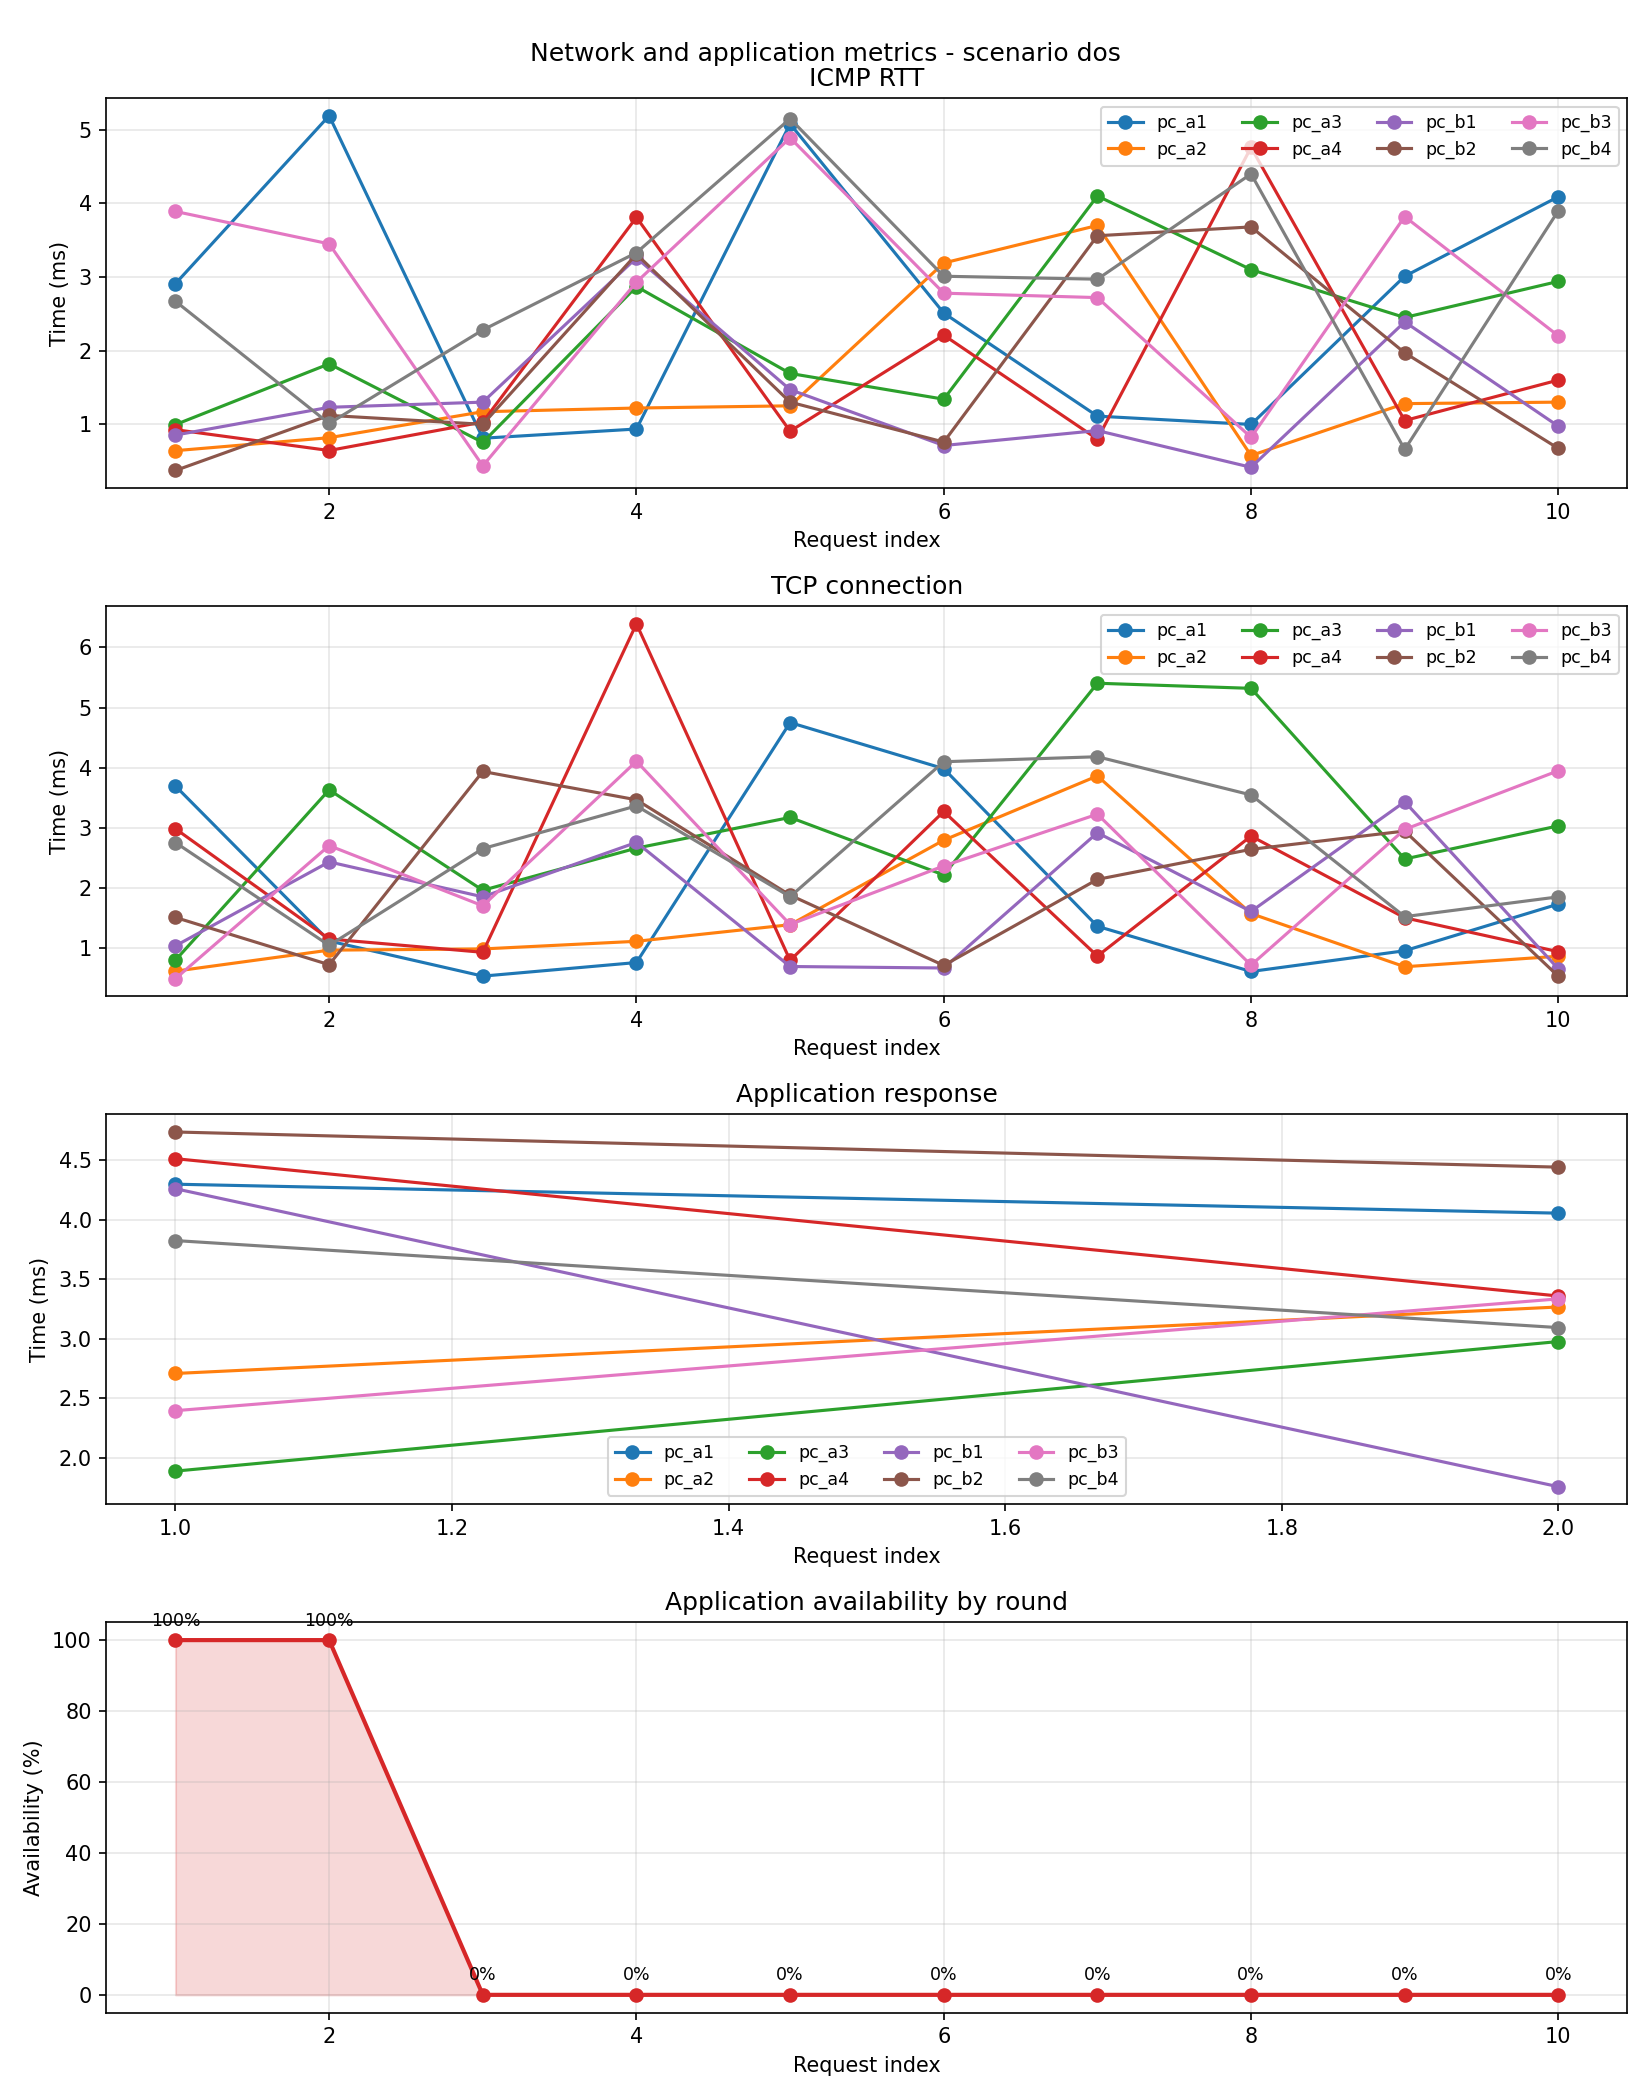
\includegraphics[width=0.90\textwidth]{images/dos_lab_simulation_0001_dos_metrics.png}
\caption{Per-client network and application measurements during the direct-server controlled-load phase in \texttt{dos\_lab/simulation\_0001}.}
\label{fig:direct-dos-metrics}
\end{figure}

Figure~\ref{fig:availability-comparison} separates the complete transition from
the workload-active interval and anticipates the mitigation comparison in
Section~\ref{sec:mitigation-results}. The plot focuses on completed application
requests rather than on ICMP or TCP reachability, because those lower-layer
checks remained successful throughout both experiments.

\begin{figure}[htbp]
\centering
\resizebox{0.98\textwidth}{!}{%
\begin{tikzpicture}[x=0.9cm,y=0.048cm]
    \draw[->] (0,0) -- (14.8,0) node[right] {Scenario};
    \draw[->] (0,0) -- (0,115) node[above] {Availability (\%)};
    \foreach \y in {0,20,40,60,80,100} {
        \draw (-0.08,\y) -- (0.08,\y) node[left=3pt] {\small \y};
    }
    \draw[fill=gray!30] (0.7,0) rectangle (2.3,100);
    \draw[fill=gray!55] (3.5,0) rectangle (5.1,20);
    \draw[line width=2.2pt] (6.3,0.8) -- (7.9,0.8);
    \draw[fill=blue!20] (9.1,0) rectangle (10.7,100);
    \draw[fill=blue!45] (11.9,0) rectangle (13.5,100);
    \node[below,align=center] at (1.5,0) {Direct\\baseline};
    \node[below,align=center] at (4.3,0) {Direct\\complete};
    \node[below,align=center] at (7.1,0) {Direct\\active};
    \node[below,align=center] at (9.9,0) {Proxy\\baseline};
    \node[below,align=center] at (12.7,0) {Proxy\\active};
    \node[above] at (1.5,100) {100\%};
    \node[above] at (4.3,20) {20\%};
    \node[above] at (7.1,1.0) {0\%};
    \node[above] at (9.9,100) {100\%};
    \node[above] at (12.7,100) {100\%};
\end{tikzpicture}
}
\caption{Application availability without and with the reverse-proxy mitigation. ``Complete'' includes the two pre-activation rounds; ``active'' denotes rounds 3--10.}
\label{fig:availability-comparison}
\end{figure}

The service-side counters explain the client observation. During the baseline,
the service recorded 80 accepted connection events and no rejected or
\texttt{BUSY} events. During the controlled-load window it recorded 56 accepted
connection events together with 264 rejected/\texttt{BUSY} events. The maximum
number of simultaneously active application connections reached exactly 20,
which is the configured semaphore limit, and the maximum active thread count
rose from four in the baseline to 25 during the load phase. Periodic server
samples recorded a mean of 15.00 active connections during the
controlled-load scenario, compared with approximately zero at the one-second
sampling instants during the short baseline transactions.

\begin{table}[htbp]
\centering
\small
\begin{tabular}{lrr}
\toprule
\textbf{Server-side observation} & \textbf{Baseline} & \textbf{Controlled load} \\
\midrule
Accepted connection events & 80 & 56 \\
Rejected / \texttt{BUSY} events & 0 & 264 \\
Maximum active connections & 1 & 20 \\
Mean active connections in periodic samples & 0.00 & 15.00 \\
Maximum active threads & 4 & 25 \\
Mean container CPU$^{\dagger}$ & 0.53\% & 2.13\% \\
Maximum container CPU$^{\dagger}$ & 0.88\% & 7.14\% \\
Maximum container memory$^{\dagger}$ & 0.05\% & 0.07\% \\
Maximum container PIDs$^{\dagger}$ & 3 & 23 \\
\bottomrule
\end{tabular}
\caption{Server and container observations for \texttt{dos\_lab/simulation\_0001}. Values marked with $^{\dagger}$ are based on six Docker-stat samples per scenario and are therefore descriptive.}
\label{tab:server-comparison}
\end{table}

The resource samples show higher CPU activity and many more processes/threads
under load, but they should not be over-interpreted. Only six Docker-stat rows
were archived for each scenario, and CPU utilisation on a shared host is
sensitive to scheduling and unrelated host activity. The stronger evidence is
the application-specific instrumentation: the service reached its configured
limit of 20 active connections and generated hundreds of overload rejections
while overall availability fell to 20\% and attack-active availability fell to
0\%. These observations are
directly related by the service implementation and do not depend on a precise
host CPU baseline.

The per-client distribution is also useful. Every legitimate client completed
two out of ten requests, corresponding to 20\% over the complete controlled
run; for every client, both successful requests occurred before workload
activation, so availability during the attack-active interval was 0\%.
There is therefore no indication that a single access LAN or routing path was
responsible for the failures. Instead, the loss of availability appears across
both client networks at the same time, consistent with contention at the common
server endpoint. Combined with the fact that all ICMP probes remained
successful, this supports the interpretation that the routing infrastructure
continued to operate while the application capacity was exhausted.

\section{Reverse-Proxy Mitigation Results}
\label{sec:mitigation-results}

The representative reverse-proxy execution evaluates the mitigation topology
under the same client schedule. A rate-limiting reverse proxy exposes the public endpoint
at \texttt{10.30.1.10:9000} and forwards admitted sessions to a backend at
\texttt{10.30.2.10:9000}. The proxy applies global and per-source connection
limits, while the clients continue to use the same application protocol and
the controlled agents retain the same activation point. Consequently, the
intentional experimental change is the protected service path rather than the
client measurement procedure.

The baseline and controlled-load files in
\path{mitigation/simulation_0002} each contain 80 requests. Every request
succeeded at the ICMP, TCP, and application layers in both phases. In
particular, all 64 legitimate requests in rounds 3--10 completed while the
controlled workload was active, compared with 0 of 64 in the direct-server
experiment. Each of the eight clients therefore achieved ten successes out of
ten, with no difference in availability between the two access LANs.

\begin{table}[htbp]
\centering
\small
\setlength{\tabcolsep}{4pt}
\begin{tabular}{lrrr}
\toprule
\textbf{Client-side metric} & \textbf{Proxy baseline} & \textbf{Proxy load} & \textbf{Direct load} \\
\midrule
Successful application requests & 80 / 80 & 80 / 80 & 16 / 80 \\
Overall application availability & 100.00\% & 100.00\% & 20.00\% \\
Attack-active availability & -- & 100.00\% & 0.00\% \\
Successful ICMP probes & 80 / 80 & 80 / 80 & 80 / 80 \\
Successful TCP handshakes & 80 / 80 & 80 / 80 & 80 / 80 \\
Mean ICMP RTT & 1.550 ms & 1.674 ms & 2.127 ms \\
Mean TCP connection time & 1.808 ms & 1.781 ms & 2.198 ms \\
Mean application response time & 6.058 ms & 5.545 ms & 3.432 ms$^{*}$ \\
Median application response time & 5.896 ms & 5.133 ms & 3.347 ms$^{*}$ \\
95th percentile application response & 9.177 ms & 9.502 ms & 4.567 ms$^{*}$ \\
Maximum application response time & 11.696 ms & 11.019 ms & 4.735 ms$^{*}$ \\
\bottomrule
\end{tabular}
\caption{Client-side results for the mitigation experiment and the corresponding direct-server load phase. Direct-load application latencies marked with $^{*}$ describe only the 16 successful requests.}
\label{tab:mitigation-client-comparison}
\end{table}

Figures~\ref{fig:mitigation-baseline-metrics} and
\ref{fig:mitigation-dos-metrics} show the complete per-client series for the
mitigation experiment. Unlike the direct-server load plot, the application
panel contains observations for every client and round, and the availability
panel remains at 100\% after workload activation.

\begin{figure}[p]
\centering
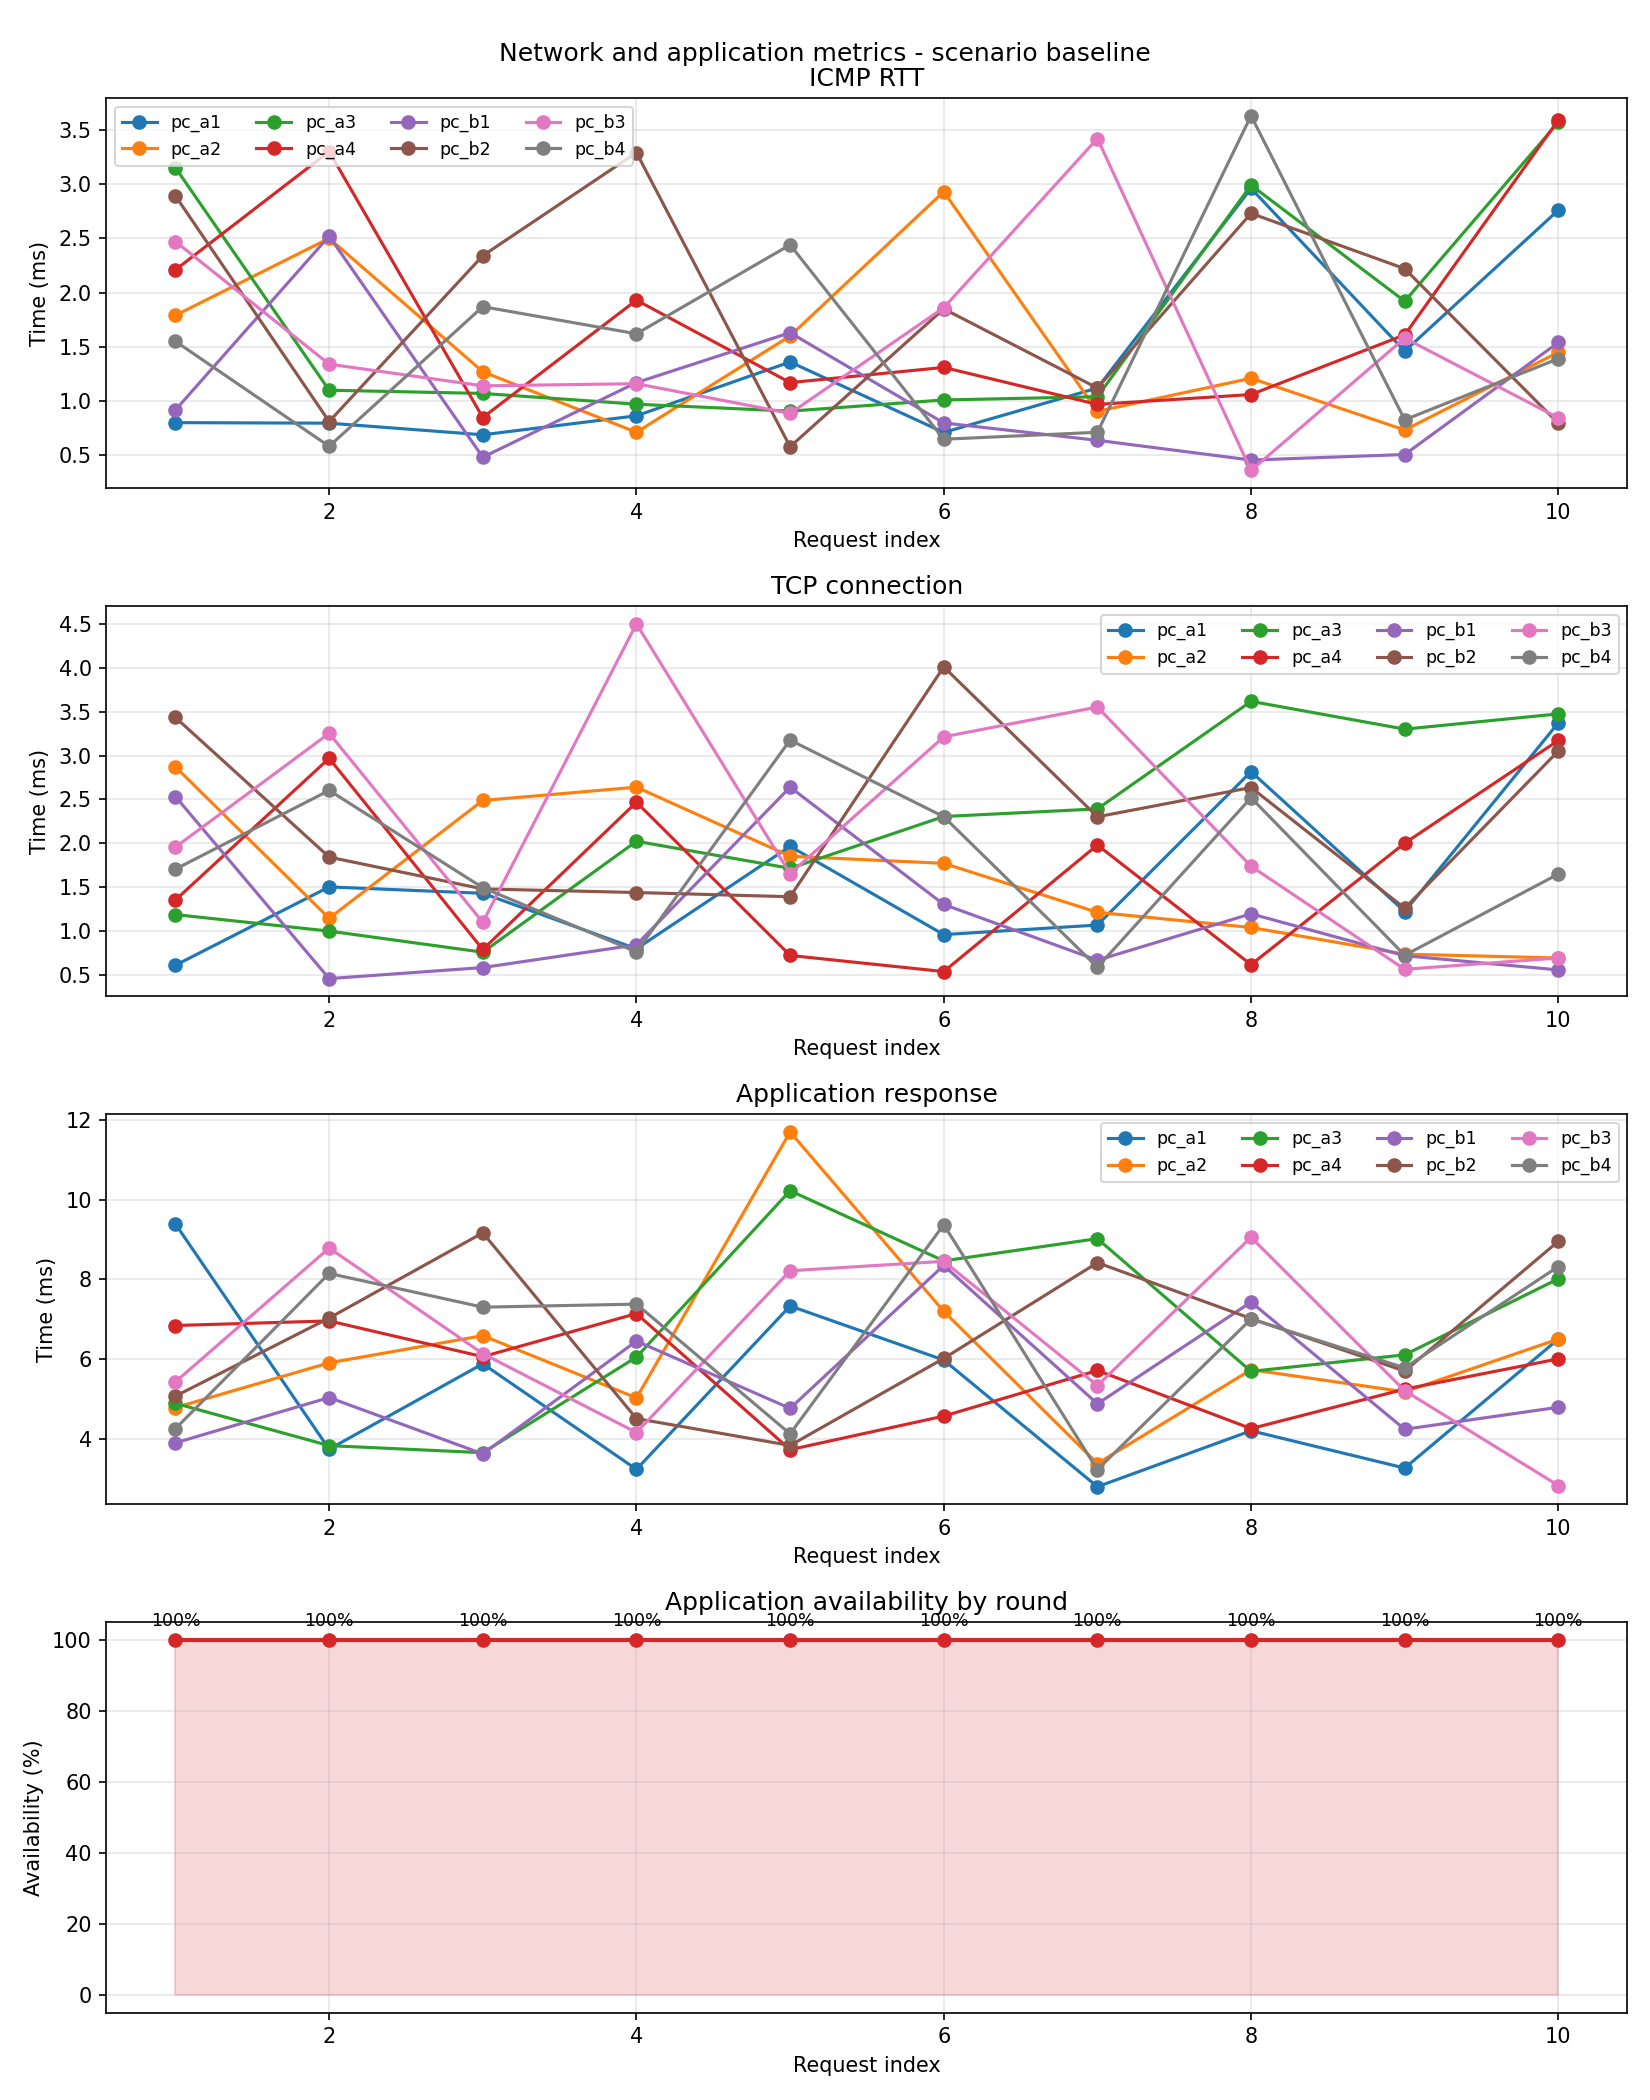
\includegraphics[width=0.90\textwidth]{images/mitigation_simulation_0002_baseline_metrics.png}
\caption{Per-client network and application measurements for the reverse-proxy baseline in \texttt{mitigation/simulation\_0002}.}
\label{fig:mitigation-baseline-metrics}
\end{figure}

\begin{figure}[p]
\centering
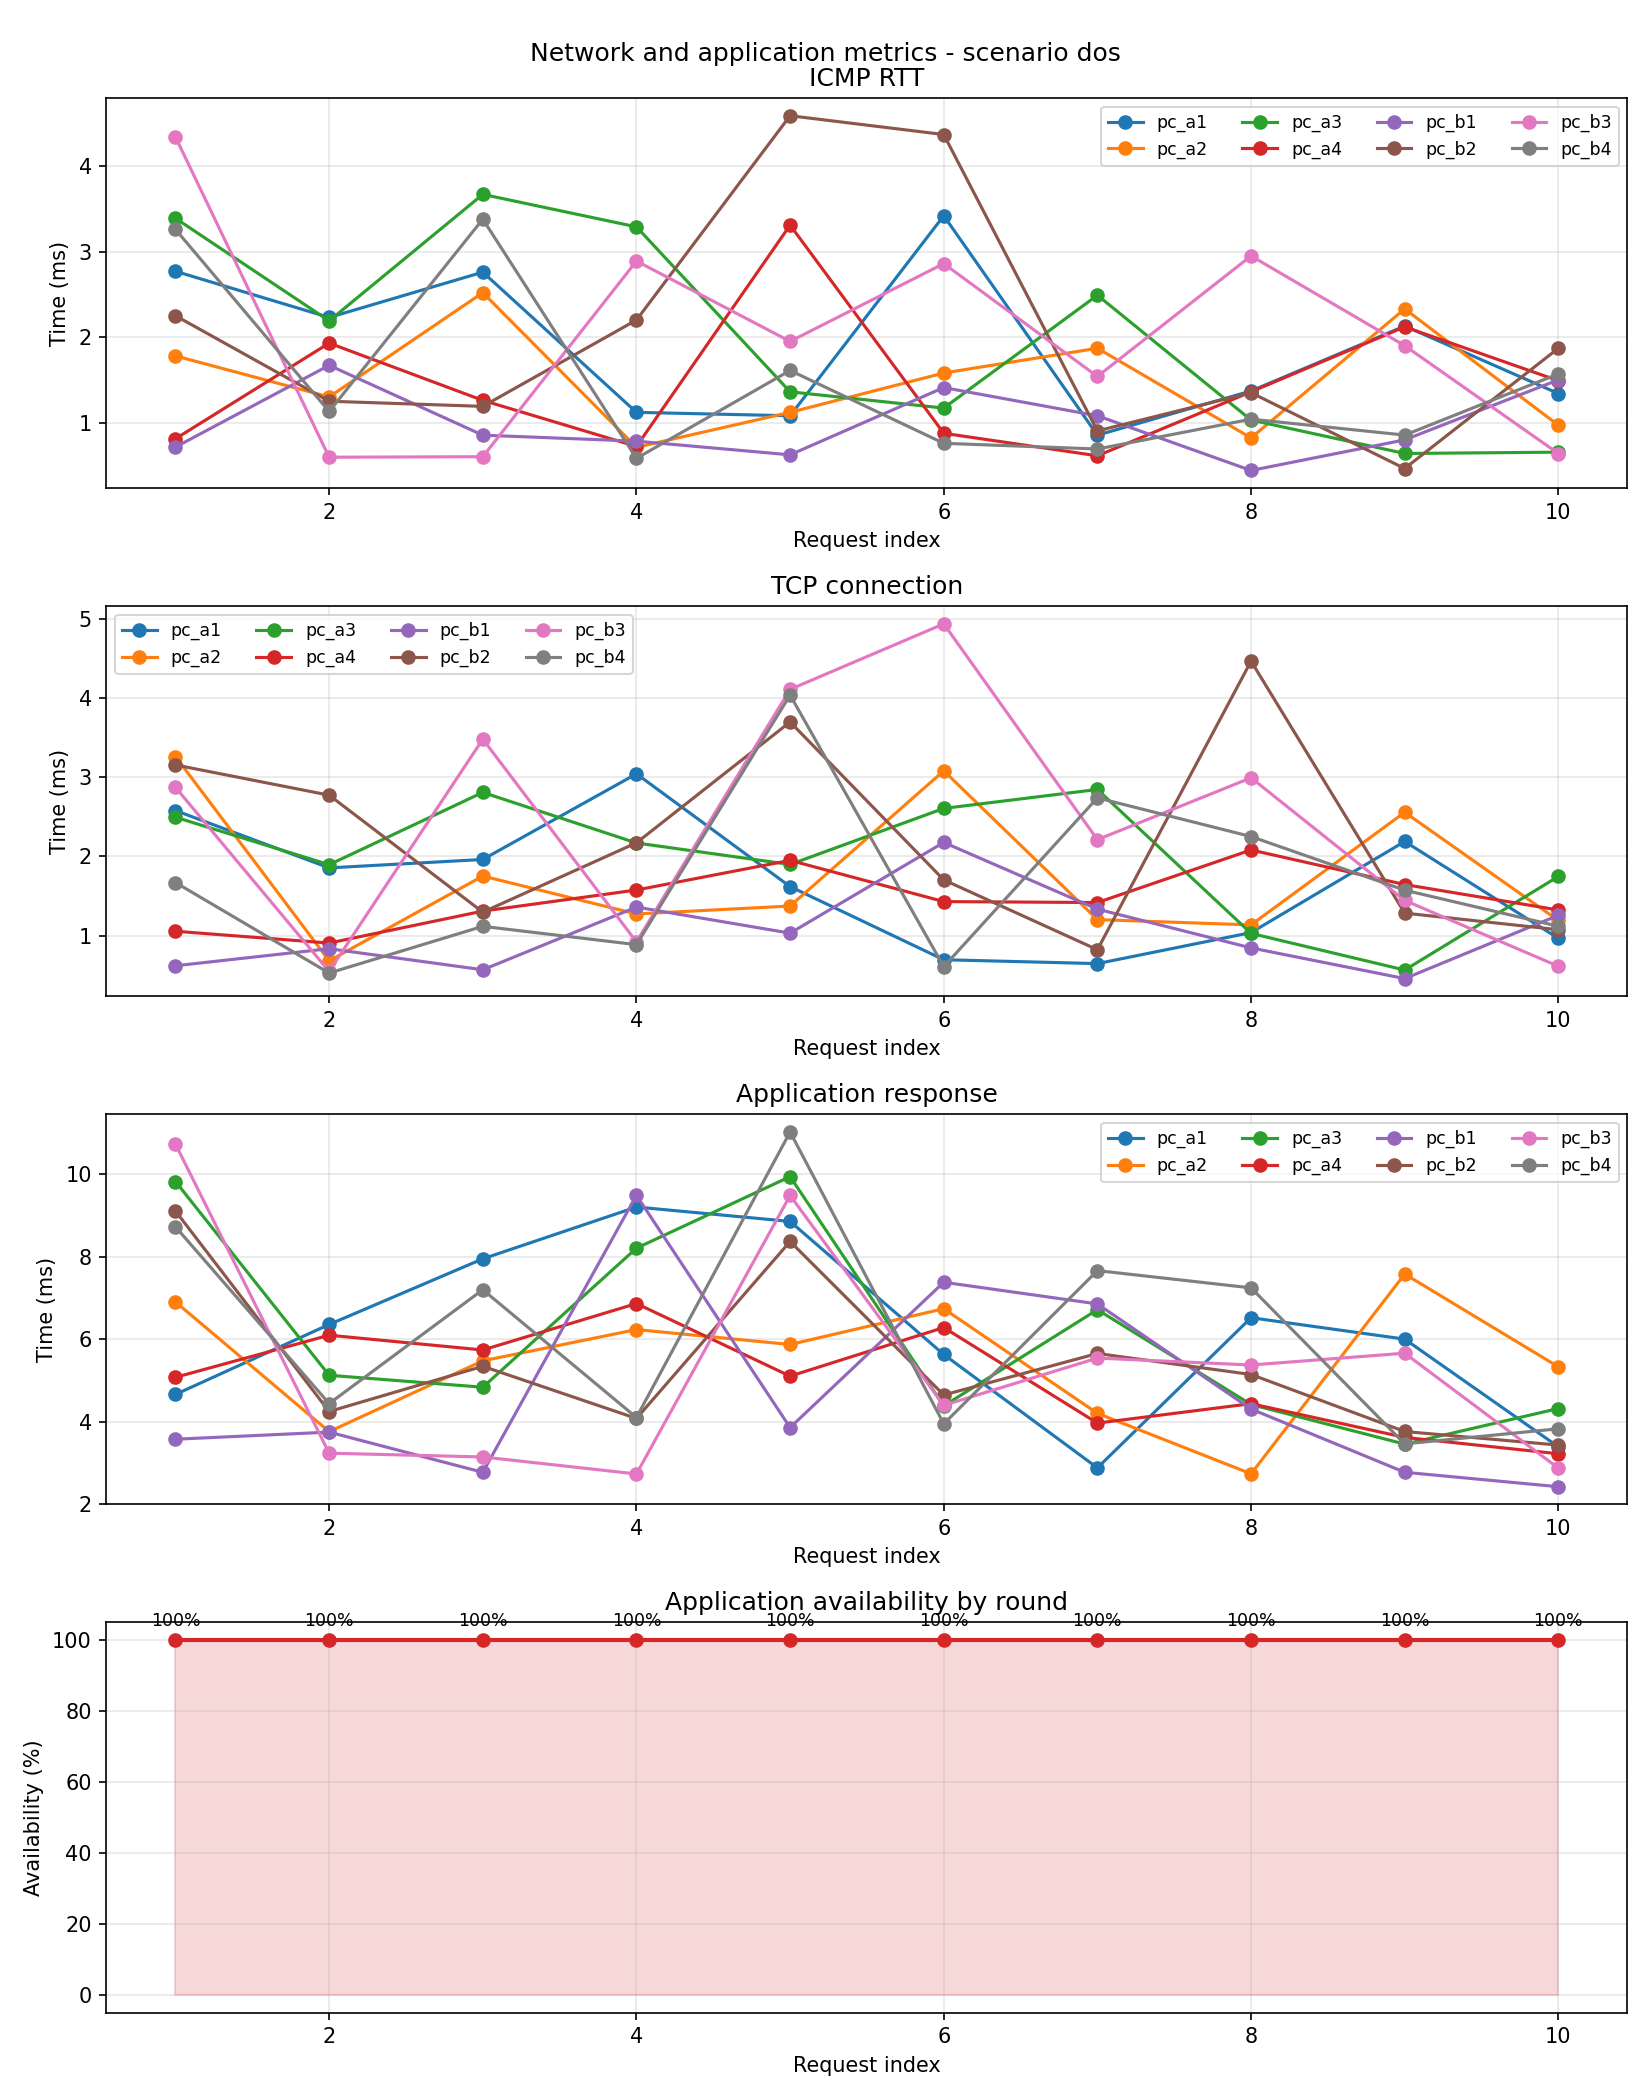
\includegraphics[width=0.90\textwidth]{images/mitigation_simulation_0002_dos_metrics.png}
\caption{Per-client network and application measurements during the reverse-proxy controlled-load phase in \texttt{mitigation/simulation\_0002}.}
\label{fig:mitigation-dos-metrics}
\end{figure}

The proxy introduces a measurable baseline cost: mean application response
time is 6.058 ms through the proxy and 3.218 ms in the direct-server baseline,
a difference of 2.840 ms. This latency difference should be interpreted as a
descriptive observation from one run, not as a stable estimate of proxy
overhead. More importantly for this experiment, the distribution remains
bounded under load: the mitigated mean is 5.545 ms and the 95th percentile is
9.502 ms while all requests complete. The lower mean under load than in the
proxy baseline is another reason not to infer small performance differences
from a single short execution.

The backend instrumentation is consistent with the client-side result. During
the mitigated load phase the backend records 92 accepted connections, no
rejected or \texttt{BUSY} event, and a maximum of eight simultaneous
connections, well below its limit of 20. The count exceeds the 80 legitimate
requests because a limited subset of controlled-workload sessions also reaches
the backend. The reverse proxy therefore does not remove all adverse traffic;
in this run it prevents that traffic from exhausting the backend's application
slots.

\begin{table}[htbp]
\centering
\small
\setlength{\tabcolsep}{4pt}
\begin{tabular}{lrrr}
\toprule
\textbf{Backend observation} & \textbf{Proxy baseline} & \textbf{Proxy load} & \textbf{Direct load} \\
\midrule
Accepted connection events & 80 & 92 & 56 \\
Rejected / \texttt{BUSY} events & 0 & 0 & 264 \\
Maximum active connections & 2 & 8 & 20 \\
Mean active connections in periodic samples & 0.00 & 4.62 & 15.00 \\
Maximum active threads & 4 & 10 & 25 \\
Mean container CPU$^{\dagger}$ & 0.49\% & 0.78\% & 2.13\% \\
Maximum container CPU$^{\dagger}$ & 0.75\% & 1.56\% & 7.14\% \\
Maximum container memory$^{\dagger}$ & 0.05\% & 0.06\% & 0.07\% \\
Maximum container PIDs$^{\dagger}$ & 3 & 9 & 23 \\
\bottomrule
\end{tabular}
\caption{Backend and container observations with mitigation, compared with the unmitigated load phase. Values marked with $^{\dagger}$ are based on six Docker-stat samples per phase.}
\label{tab:mitigation-server-comparison}
\end{table}

These results demonstrate effectiveness only for the bounded,
connection-oriented workload and rate limits used in this laboratory. They do
not establish resistance to volumetric traffic, source-address rotation,
distributed sources that defeat per-source limits, proxy resource exhaustion,
or the application-layer techniques discussed earlier in the chapter. The
representative pair shows that attack-active application availability increases
from 0\% without the proxy to 100\% with it, while the backend maximum falls
from 20 to eight simultaneous connections and overload rejections fall from
264 to zero. Whether these values persist across clean laboratory restarts is
evaluated explicitly in Section~\ref{sec:repeated-run-validation}.

The experiment demonstrates why the measurement framework records several
layers independently. ICMP RTT answers whether the host is reachable; TCP
connection time describes connection establishment; application response time
measures successful transactions; application status captures whether the
transaction actually completed; and server-side counters reveal the internal
capacity state. No single metric is sufficient to describe the experiment. The
combination makes it possible to identify a state in which the network remains
healthy, TCP remains reachable, but the application is no longer reliably
available to legitimate clients.


\section{Repeated-Run Repeatability Analysis}
\label{sec:repeated-run-validation}

To evaluate run-to-run repeatability, the complete baseline and controlled-load
procedure was executed five times for each topology. The runs were organised
as five acquisition blocks, each containing one direct-server run and one
reverse-proxy run; the laboratory was cleaned and restarted between
executions. Client count, round count, timeouts, workload activation point,
number of controlled connection workers, and workload duration were unchanged.
The direct run preceded the mitigated run inside each block, so the pairing
controls the acquisition period but does not remove every possible host-order
effect.

The statistical unit is one complete execution, not one of its 80 client
requests. Request-level observations within a run are dependent because they
share the same emulated network, server process, host scheduler, and workload
episode. Each run was therefore summarised first; descriptive statistics were
then calculated across the five run-level values. Table~\ref{tab:repeated-run-summary}
reports the median, first and third quartiles, and sample variance $s^2$ with
denominator $n-1$. Percentiles within each run use the same nearest-rank method
as \path{show_connection_results.py}. For availability under active load, only
rounds 3--10 are included, yielding 64 legitimate requests per run.

\begin{table}[htbp]
\centering
\small
\setlength{\tabcolsep}{3.5pt}
\begin{tabular}{>{\raggedright\arraybackslash}p{0.32\textwidth}rr@{\hspace{7pt}}rr}
\toprule
& \multicolumn{2}{c}{\textbf{Direct server}} & \multicolumn{2}{c}{\textbf{Reverse proxy}} \\
\cmidrule(lr){2-3}\cmidrule(lr){4-5}
\textbf{Run-level metric} & \textbf{Median [Q1, Q3]} & \boldmath{$s^2$} & \textbf{Median [Q1, Q3]} & \boldmath{$s^2$} \\
\midrule
Baseline availability (\%)
& 100 [100, 100] & 0
& 100 [100, 100] & 0 \\
Active-load availability (\%)
& 0 [0, 0] & 0
& 100 [100, 100] & 0 \\
Baseline application median (ms)
& 3.335 [3.290, 3.336] & 0.088
& 5.808 [5.437, 5.896] & 0.144 \\
Baseline application p95 (ms)
& 5.399 [5.008, 5.900] & 0.338
& 9.514 [9.170, 10.915] & 1.899 \\
Active-load application median (ms)
& -- & --
& 5.315 [5.236, 5.700] & 0.271 \\
Active-load application p95 (ms)
& -- & --
& 9.481 [9.151, 9.540] & 0.663 \\
Rejected / \texttt{BUSY} events
& 264 [264, 264] & 0
& 0 [0, 0] & 0 \\
Maximum active backend connections
& 20 [20, 20] & 0
& 8 [8, 8] & 0 \\
\bottomrule
\end{tabular}
\caption{Run-level descriptive statistics across five complete executions per topology. Variance is the sample variance across runs. Dashes denote an undefined latency statistic because no direct-server request completed during active load.}
\label{tab:repeated-run-summary}
\end{table}

Figure~\ref{fig:repeated-run-comparison} displays the observed run-level values
directly, without fitting a distribution to the five executions. The paired
layout preserves the acquisition-block structure and separates quantities with
different units into distinct panels.

\begin{figure}[p]
    \centering
    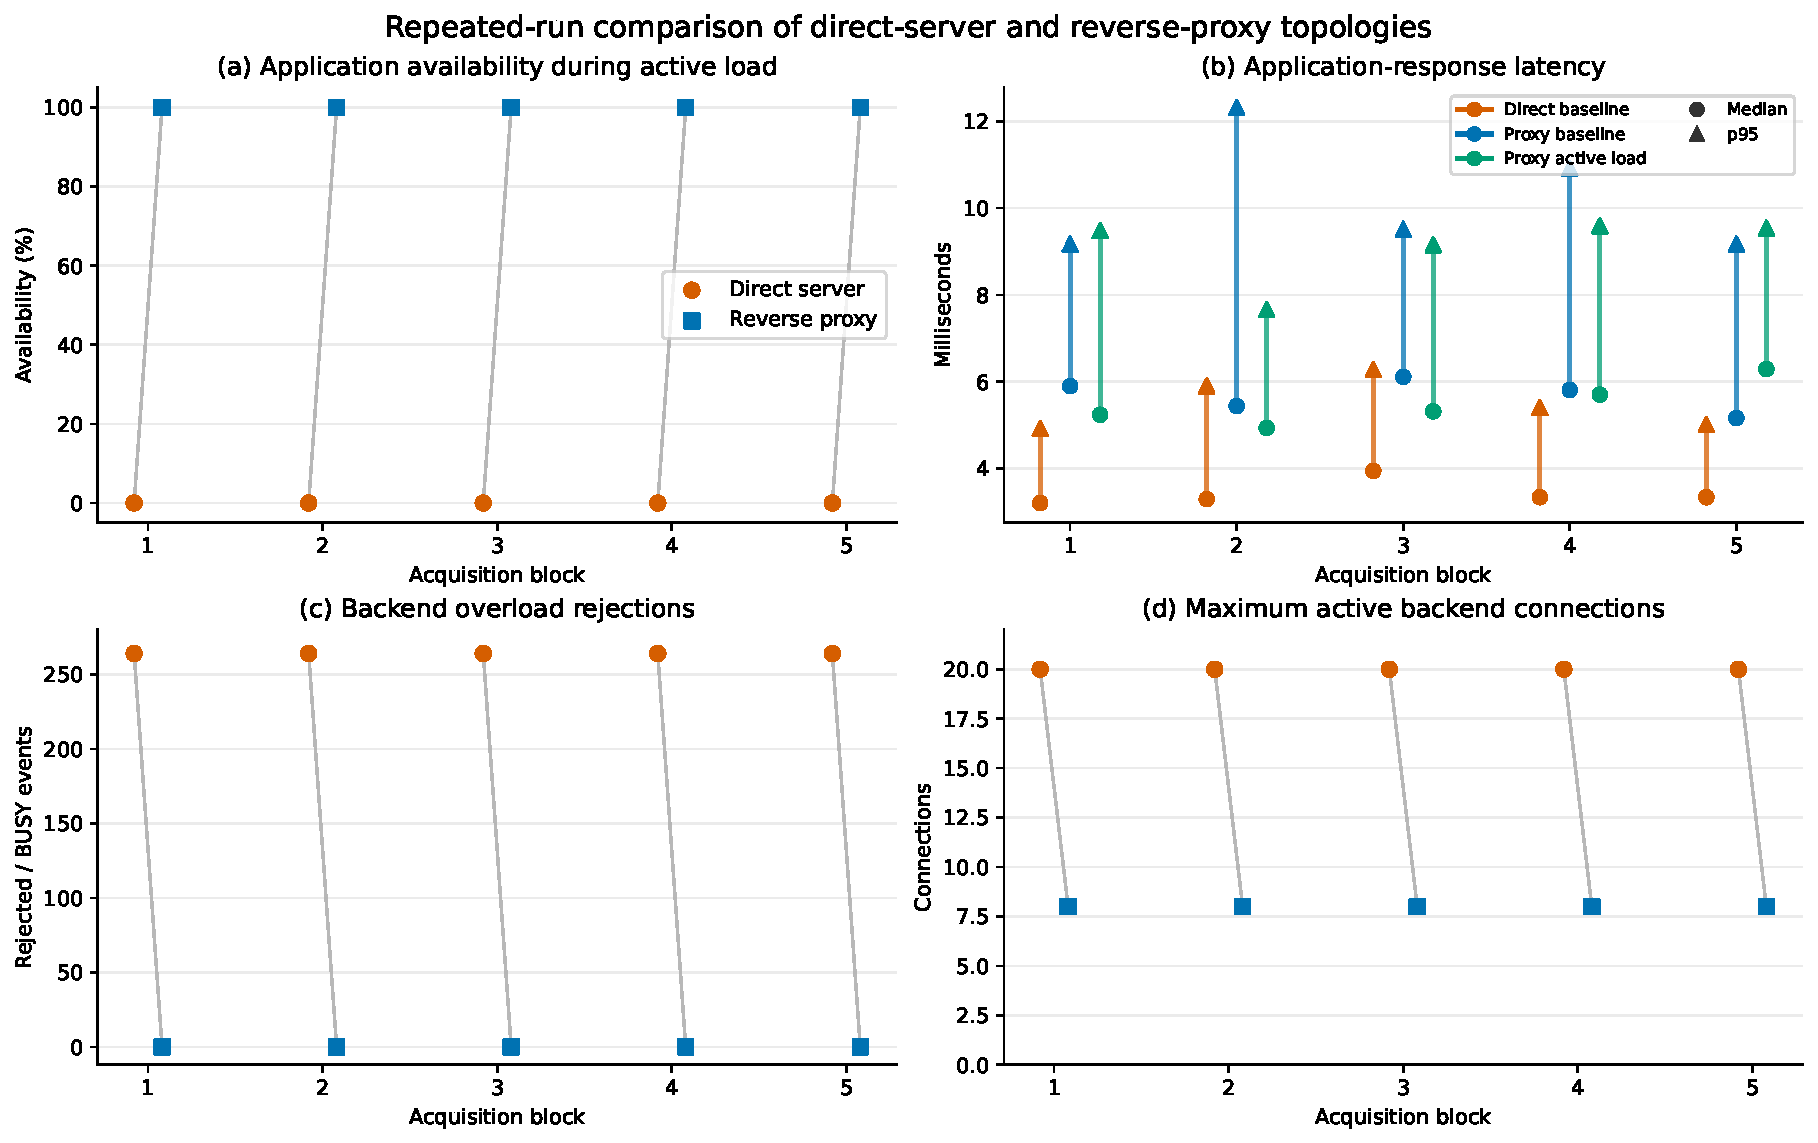
\includegraphics[width=\textwidth]{images/repeated_run_validation.pdf}
    \caption{Run-level comparison across the five paired acquisition blocks.
    Grey lines connect the direct-server and reverse-proxy observations within
    each block. Panel~(a) reports attack-active application availability;
    panel~(b) reports application-response medians and p95 values where a
    transaction completed; panels~(c) and~(d) report backend overload
    rejections and maximum active connections. Direct-server active-load
    latency is absent because no request completed during that interval.}
    \label{fig:repeated-run-comparison}
\end{figure}

All five direct-server baselines and all five reverse-proxy baselines achieved
80 successes out of 80 requests. During the complete transition phase, every
direct-server run achieved 16 successes out of 80, because only the two
pre-activation rounds completed. Consequently, all five direct-server runs had
0 successes out of 64 during active load. In contrast, every reverse-proxy run
completed all 64 active-load requests. The paired availability difference was
therefore $+100$ percentage points in each of the five acquisition blocks:
median $+100$, interquartile interval $[+100,+100]$, and sample variance zero.
This exact replication provides evidence of consistent behaviour for the
tested configuration beyond the original single execution, although five runs
remain a small sample and do not justify extrapolation to other workload
models.

Latency is reported only where an application transaction completed. No
direct-server application latency exists for rounds 3--10, so assigning a
timeout value or comparing the proxy only with the 16 pre-activation direct
successes would bias the result. The protected path instead produced an
active-load median response between 4.934 and 6.288 ms across runs and a p95
between 7.661 and 9.590 ms. In the baseline, the paired increase in the
per-run application median introduced by the proxy had a median of 2.167 ms
and an interquartile interval of [2.147, 2.472] ms. This provides a run-level
estimate of the protection overhead while keeping availability and latency as
separate outcomes.

The server-side evidence is equally stable. Every direct run reached the
20-connection application limit and recorded 264 rejected or \texttt{BUSY}
events during the controlled-load phase. Every mitigated run limited the
backend maximum to eight connections and recorded zero overload rejection.
Thus each paired block reduced the maximum backend occupancy by 12 connections
and the rejection count by 264. The zero variances in these discrete outcomes
describe deterministic repetition under the fixed laboratory parameters; they
must not be interpreted as proof that the same values hold for untested rates,
source populations, protocols, or host environments.

\section{Threats to Validity}
\label{sec:experimental-threats-validity}

The results support a comparison between the two implemented architectures
under the stated parameters, but several threats constrain their
interpretation.

\paragraph{Construct validity.}
Application availability is defined as receipt of the expected response within
the configured timeout. This is stronger than ICMP reachability or completion
of a TCP handshake, but it represents one small TCP service rather than every
notion of service quality. Response time is defined only for completed
transactions; failed requests are therefore reported through availability and
are not assigned an artificial latency. The controlled workload reproduces a
bounded application-layer resource-exhaustion condition generated by known
nodes. It is useful for comparing the direct and protected paths, but it is not
a measurement of Internet-scale DDoS resistance.

\paragraph{Internal validity.}
Both emulated networks, their containers, and the measurement processes share
one physical host. CPU scheduling, filesystem activity, and Docker overhead
can consequently affect clients, workload generators, proxy, and server at the
same time. Pairing the two architectures within acquisition blocks reduces
changes between distant measurement periods, and cleaning and restarting the
laboratory reduces residual runtime state. However, the direct-server run
always preceded the proxy run inside a block, so an order or warm-cache effect
cannot be excluded. The proxy topology also adds both rate limiting and an
extra processing hop; the experiment estimates the effect of the complete
architectural change and does not isolate every proxy mechanism individually.

\paragraph{External validity.}
The experiment uses Kathar\'a and Docker on one workstation, a fixed routed
topology, eight legitimate clients, one application protocol, one server
capacity limit, and one controlled workload profile. Different machines,
container runtimes, network delays, loss patterns, request mixes, proxy rules,
or adversarial strategies may produce different results. In particular, a
distributed workload with many source identities could interact differently
with rate limiting. The observed 0\% and 100\% active-load availability values
therefore characterise the tested configurations and must not be extrapolated
to production services.

\paragraph{Conclusion validity.}
Five paired executions provide stronger evidence than a single demonstration,
and treating each complete run as the statistical unit avoids presenting the
dependent client requests as independent samples. Nevertheless, five pairs are
too few for precise population estimates or a persuasive analysis of small
latency differences. The repeated binary and counter outcomes are reported
descriptively; zero sample variance records what occurred in these runs, not an
absence of variability in the wider population. Further evaluation should
randomise execution order, increase the number of independent restarts, and
vary workload intensity and host conditions before making broader causal or
performance claims.

\section{Chapter Summary}
\label{sec:experimental-summary}

This chapter evaluated the generated framework through a controlled experiment
executed entirely inside Kathar\'a. The testbed combined eight legitimate
clients, an OSPF-based routed core, a separate workload network, and an
instrumented TCP application service. The orchestration layer verified target
reachability before measurement, executed all legitimate clients concurrently
for each round, and stored client, application, server, and container metrics
under a run-specific directory.

Across all five direct-server runs, every baseline produced 80 successful
application transactions out of 80 attempts. Every complete transition run had
20\% availability because its first two rounds preceded workload activation;
during rounds 3--10, every run had 0 successes out of 64 despite successful
ICMP probes and TCP handshakes. In all five executions the service reached its
configured limit of 20 active connections and recorded 264 overload
rejections. The repeated result demonstrates a distinction that is central to
end-to-end service evaluation: network reachability and TCP acceptance do not
necessarily imply application availability.

The five reverse-proxy runs provide the corresponding architectural
comparison. Every baseline and controlled-load phase completed all 80
application requests, including all 64 requests issued during active load. In
each run the protected backend recorded no overload rejection and reached at
most eight simultaneous connections. The paired improvement in active-load
availability was 100 percentage points in every acquisition block, while the
median baseline application-response overhead was 2.167 ms. For the bounded
workload used here, the proxy therefore preserved application availability at
the cost of higher baseline response time. This is repeated evidence for the
tested configuration, not a claim of general DDoS resistance.

The real-world cases discussed at the beginning of the chapter clarify the
scope of this result. Mirai/Dyn provides a structural example of distributed
sources, the GitHub incident illustrates reflection and amplification, HTTP/2
Rapid Reset illustrates application-layer request pressure, and the 2025
Cloudflare case illustrates hyper-volumetric short-duration flooding. The
Kathar\'a experiment does not reproduce those Internet-scale mechanisms.
Rather, it isolates a common availability principle in a controlled setting:
when offered workload exceeds a finite service resource, legitimate
transactions can fail even while lower-layer connectivity remains available.

The results also validate the usefulness of the framework as an experimental
platform. The topology is generated from YAML, the same clients and target can
be reused across scenarios, measurements are executed with a consistent schema,
and runs can be checked using explicit reachability and completion criteria.
Five repeated acquisition blocks show that the principal availability and
backend-capacity outcomes are stable across clean laboratory restarts, while
the reported quartiles and variances make the remaining latency dispersion
explicit.


\chapter{Robustness, Security Limitations and Scalability Evaluation}
\label{chap:robustness-security-scalability}

The previous chapters presented the configuration model, the validation
pipeline, the generation of Kathar\'a artefacts, and the experimental use of
the framework. This chapter evaluates the framework from a different
perspective. Rather than considering only whether a valid laboratory can be
generated, it investigates how the translator behaves when its input becomes
large, structurally complex, ambiguous, or potentially unsafe.

From the perspective of the software-development lifecycle introduced in
Section~\ref{sec:software-development-lifecycle}, this chapter represents a
final verification stage. Earlier iterations primarily asked whether the
framework could generate and execute the intended laboratories. The tests below
instead challenge assumptions made during implementation and ask what happens
when the same mechanisms are exercised with large, malformed, ambiguous, or
potentially unsafe inputs. The resulting observations are therefore feedback on
the design choices described in Chapters~\ref{chap:requirements-architecture}--\ref{chap:laboratory-generation}, not only a list of independent limitations.

The analysis has two objectives. The first is to identify scalability limits
through reproducible stress tests. The second is to discuss implementation
choices that may become robustness or security weaknesses when configuration
files are malformed or originate from an untrusted source. These two aspects
are related. A configuration language is not only a convenient input format:
it is also an interface through which a user can request the creation of
thousands of nodes, routes, routing statements, files, and startup commands.

It is important to distinguish three categories throughout this chapter.
A \emph{security vulnerability} is a behaviour that can become exploitable
across an explicit trust boundary. A \emph{robustness weakness} is a condition
that can result in an incorrect or misleading laboratory without necessarily
creating a security compromise. A \emph{model limitation} is a deliberate or
implicit restriction in the set of networks that the translator can
represent. Not all limitations described below should therefore be interpreted
as exploitable vulnerabilities.

\section{Stress-Test Methodology}
\label{sec:stress-methodology}

The descriptive scalability benchmarks exercise the translator itself rather
than the runtime scalability of Docker or Kathar\'a. Each input is therefore processed
in two modes. The first uses the framework's validation-only option and
measures YAML loading, structural validation, and semantic validation without
creating a laboratory. The second performs complete generation and additionally
writes \texttt{lab.conf}, node startup files, and FRRouting files where
required. Starting the resulting containers is intentionally outside the scope
of these measurements because it would mix translator performance with Docker,
Kathar\'a, kernel, and host-resource limitations.

The benchmark data used in this chapter are the results recorded in
\path{final_benchmark.csv} and \path{final_summary.csv}. The CSV data
contain two measured repetitions for each available scenario and mode. No
measured execution reached a timeout. Every valid configuration returned exit
code 0 in both repetitions. The intentionally invalid configuration returned
exit code 1 in both repetitions, as expected. Because two repetitions cannot
support strong distributional or inferential claims, the measurements are used
only as descriptive observations of the tested executions.

The scenarios were selected so that different dimensions of input complexity
could be isolated rather than increasing only the number of nodes:

\begin{itemize}
    \item \texttt{flat\_10000.yml}: 10,000 nodes sharing a large flat
    topology, intended to stress node and address processing without creating
    thousands of distinct collision domains;
    \item \texttt{star\_4000.yml}: approximately 4,000 nodes arranged around
    a central router with a separate point-to-point collision domain for each
    peripheral connection, intended to stress subnet and collision-domain
    validation;
    \item \texttt{chain\_1000.yml}: 1,000 routers connected in a chain,
    stressing repeated routed-node and interface generation;
    \item \texttt{enterprise\_100r\_10h.yml}: 100 routers with ten hosts per
    routed LAN, providing a more realistic mixed topology;
    \item \texttt{dense\_500.yml}: 500 routers with multiple inter-router
    links, increasing interface density;
    \item \texttt{ospf\_1000.yml}: 1,000 OSPF routers, stressing FRRouting
    validation and configuration generation;
    \item \texttt{routes\_20000.yml}: a configuration dominated by 20,000
    static-route declarations;
    \item \texttt{commands\_100000.yml}: a configuration dominated by 100,000
    custom startup commands;
    \item \texttt{large\_yaml\_15mb.yml}: a 15.64 MiB YAML configuration,
    intended to stress deserialisation and in-memory representation;
    \item \texttt{invalid\_5000.yml}: 5,000 intentionally invalid nodes,
    intended to verify that large erroneous inputs are rejected without
    producing a laboratory.
\end{itemize}

For each measured run the benchmark records elapsed time, peak resident memory,
exit status, input size, number of generated files, and output size. Table
\ref{tab:stress-results} reports the aggregated values contained in the
provided summary CSV. Times are medians of the two recorded repetitions, while
memory is the maximum peak RSS observed in those repetitions.

\begin{table}[htbp]
\centering
\scriptsize
\resizebox{\textwidth}{!}{%
\begin{tabular}{lrrrrrrr}
\toprule
\textbf{Scenario} &
\textbf{Validate (s)} &
\textbf{Generate (s)} &
\textbf{Val. RSS (MiB)} &
\textbf{Gen. RSS (MiB)} &
\textbf{Input (MiB)} &
\textbf{Files} &
\textbf{Output (MiB)} \\
\midrule
Flat 10,000 nodes       & 4.065  & 8.840  & 97.04 & 109.16 & 1.127  & 10004 & 1.146 \\
Star 4,000 nodes        & 14.565 & 29.570 & 60.69 & 67.36  & 0.688  & 4004  & 0.727 \\
Chain 1,000 routers     & 1.320  & 2.835  & 27.03 & 28.66  & 0.165  & 4001  & 0.579 \\
Enterprise 100r/10h     & 0.535  & 1.095  & 25.53 & 26.96  & 0.141  & 1401  & 0.185 \\
Dense 500 routers       & 1.235  & 2.520  & 24.79 & 26.29  & 0.135  & 2001  & 0.347 \\
OSPF 1,000 routers      & 1.730  & 3.695  & 35.38 & 37.88  & 0.292  & 4001  & 0.675 \\
20,000 static routes    & 2.900  & 5.920  & 82.34 & 92.83  & 1.020  & 6     & 0.867 \\
100,000 commands        & 4.410  & 8.645  & 76.81 & 87.23  & 3.709  & 2     & 2.946 \\
Large YAML              & 7.610  & 15.240 & 74.47 & 124.36 & 15.640 & 2     & 15.030 \\
Invalid 5,000 nodes     & 2.025  & --     & 57.04 & --     & 0.595  & 0     & 0 \\
\bottomrule
\end{tabular}}
\caption{Descriptive stress-test results from the supplied benchmark CSV
files. Times are medians of two raw measurements and should not be interpreted
as stable population estimates.}
\label{tab:stress-results}
\end{table}

The results show that node count alone is not a sufficient predictor of
translation cost. The clearest example is the comparison between the flat and
star topologies. The flat topology contains 10,000 nodes and validates in
4.065 seconds. The star topology contains only about 4,000 nodes but requires
14.565 seconds for validation. It is therefore approximately 3.6 times slower
despite containing substantially fewer nodes. Complete generation exhibits the
same effect: 8.840 seconds for the 10,000-node flat case and 29.570 seconds for
the 4,000-node star case.

This difference is explained by the semantic checks performed on collision
domains. The validator compares the subnets associated with different
collision domains in order to reject overlapping Layer~3 address spaces.
When a topology contains a very large number of distinct point-to-point
domains, the number of pairwise comparisons can grow approximately as

\[
    \frac{D(D-1)}{2},
\]

where \(D\) is the number of collision domains being compared. In the
worst case this corresponds to quadratic growth, \(O(D^2)\). A flat topology,
by contrast, may contain many nodes while keeping \(D\) small. The stress
results therefore identify the number of distinct collision domains as a more
important scalability factor than raw node count for this part of semantic
validation.

The tests dominated by configuration volume reveal a different limit. The
20,000-route configuration validates in 2.900 seconds and reaches 82.34 MiB
peak RSS, while the 100,000-command configuration validates in 4.410 seconds
and reaches 76.81 MiB. The 15.64 MiB YAML file requires 7.610 seconds for
validation and reaches 74.47 MiB during validation. During complete generation
its peak RSS rises to 124.36 MiB, the highest value in the supplied summary.
These cases indicate that large nested YAML structures impose a cost even when
the logical topology is simple, because the complete document must be
deserialised into Python dictionaries and lists before semantic processing can
begin.

Another consistent result is the relationship between validation and complete
generation time. Across all valid scenarios, the ratio between the median
generation time and the median validation time ranges from approximately
1.96 to 2.17, with a mean close to 2.06. This behaviour is consistent with the
current implementation, in which normal execution validates the configuration
at the command-line boundary and the lower-level generation function loads and
validates it again before writing files. The duplicated validation gives
\texttt{generate\_lab()} an independent safety property, because the function
does not assume that its caller has already validated the input. However, the
stress tests show that this design also becomes measurable overhead for large
configurations.

Finally, \texttt{invalid\_5000.yml} provides a useful negative result. Both
recorded executions terminated in about 2.02--2.03 seconds with exit code 1,
without timeout and without generating output files. This demonstrates that
the validation pipeline can reject a large erroneous configuration without
continuing into the generation phase. From a robustness perspective this is a
positive property.

\section{Security and Robustness Weaknesses}
\label{sec:translator-weaknesses}

The stress tests identify performance boundaries, but other weaknesses arise
from the expressive features of the configuration language itself. Several of
these features are deliberate escape mechanisms. They are useful when YAML
files are trusted and authored by the laboratory designer, but they create a
clear trust boundary if configurations are downloaded, shared, or generated by
another user.

\paragraph{Arbitrary startup commands.}
The most important security-sensitive feature is the \texttt{commands} list.
Each command string is copied literally to the node startup file. This is
intentionally flexible: it allows the framework to launch applications,
configure kernel parameters, create files, or perform operations not covered
by the declarative model. It also means that a YAML file can carry executable
shell commands.

A harmless proof-of-concept configuration is:

\begin{lstlisting}[caption={Benign demonstration of command execution through a startup entry.},
label={lst:command-execution-example}]
nodes:
  pc_a:
    type: host
    interfaces:
      - network: lan_a
        ip: 10.0.1.10/24
    commands:
      - echo "COMMAND_EXECUTED" > /tmp/translator_test
\end{lstlisting}

The generated \texttt{pc\_a.startup} file contains the command literally. When
the laboratory starts, the command executes inside the node container. This
should not be described as an automatic host compromise: execution occurs in
the container context, and escalation beyond that boundary depends on the
container configuration and runtime privileges. Nevertheless, if YAML is
accepted from an untrusted source, the feature becomes a command-execution
boundary and should be treated accordingly.

A theoretical mitigation is to introduce two operating modes. A strict or
safe mode would reject \texttt{commands} entirely and permit only structured
operations represented by dedicated YAML fields. An explicit
\cliopt{allow-commands} option could retain the current behaviour for trusted
laboratories. Common operations currently expressed as shell strings could
progressively be converted into typed fields. Additional protection could
include command allowlists, clear warnings when a configuration contains
opaque commands, and reduced Linux capabilities for containers that do not
need privileged operations.

\paragraph{Opaque commands can bypass semantic intentions.}
The parser performs only limited consistency checks on command strings. For
example, it can recognise some explicit attempts to disable IPv4 forwarding on
a node declared as a router. General shell semantics, however, cannot be
reliably inferred from text. Equivalent operations can be written in many
forms. A configuration such as

\begin{lstlisting}[caption={Equivalent command that changes a forwarding runtime property.},
label={lst:forwarding-bypass-example}]
r1:
  type: router
  forwarding: true
  interfaces:
    - network: lan_a
      ip: 10.0.1.1/24
    - network: lan_b
      ip: 10.0.2.1/24
  commands:
    - sh -c 'echo 0 > /proc/sys/net/ipv4/ip_forward'
\end{lstlisting}

illustrates the general problem. The declarative field states that the node is
intended to forward traffic, while a later opaque command can change the
runtime state. In addition, \texttt{forwarding: true} currently expresses
intent and validation consistency but does not itself emit a kernel
\texttt{sysctl} operation.

The general solution is not to build an increasingly complex regular
expression for shell commands. A stronger design would make forwarding a
generated postcondition: when \texttt{forwarding: true} is selected, the
generator could explicitly configure the kernel state at a well-defined stage
and optionally verify it after startup. In strict mode, commands that directly
modify protected networking parameters could be disallowed.

\paragraph{Raw FRRouting configuration bypasses most semantic guarantees.}
The \texttt{frr.config} field provides another intentional escape mechanism.
Instead of generating protocol blocks from structured YAML fields, the
framework writes user-provided FRRouting text directly to
\texttt{frr.conf}. This is useful for advanced FRR features not represented by
the declarative model, but the translator cannot fully validate the semantics
of arbitrary FRR syntax.

For example:

\begin{lstlisting}[caption={Raw FRR content that cannot be fully validated by the YAML model.},
label={lst:raw-frr-example}]
frr:
  config: |
    router ospf
     this-command-does-not-exist
\end{lstlisting}

can be syntactically valid YAML while still containing an invalid FRR command.
Successful YAML translation therefore does not imply successful FRR startup.

A possible mitigation is to distinguish generated FRR configuration from raw
FRR configuration in the validation report and mark the latter as
``unverified''. A stricter implementation could invoke the FRR parser in a
disposable validation environment before accepting the laboratory. Another
option is to disable \texttt{frr.config} in strict mode and require the
structured protocol model whenever reproducibility and static validation are
more important than maximum expressiveness.

\paragraph{Static-route next hops are less deeply validated.}

Interfaces and default gateways receive strong semantic checks, including address parsing and directly connected gateway validation. Arbitrary static routes are less extensively analysed. Consider a router connecting two different networks:

\begin{lstlisting}[caption={Static route with a next hop outside the router's connected subnets.},
label={lst:static-route-weakness}]
r1:
  type: router
  interfaces:
    - network: lan_a
      ip: 10.0.1.1/24
    - network: lan_b
      ip: 10.0.2.1/24

  routes:
    - to: 172.16.0.0/16
      via: 192.168.200.1
\end{lstlisting}

The router is directly connected only to the \texttt{10.0.1.0/24} and \texttt{10.0.2.0/24} networks. However, the static route specifies \texttt{192.168.200.1} as its next hop, even though that address is not reachable through either configured interface.

The route can still be translated into:

\begin{lstlisting}[language=bash]
ip route add 172.16.0.0/16 via 192.168.200.1
\end{lstlisting}

Consequently, the YAML configuration may be accepted and translated even though the resulting route is operationally incorrect.

A possible improvement would be to apply to every \texttt{routes[].via} field a reachability check similar to the one already used for \texttt{default\_gateway}. The validator could verify that the next-hop address belongs to at least one subnet directly connected to the router. More advanced cases, such as explicitly configured \texttt{onlink} routes or recursive next-hop resolution, could later be supported through dedicated configuration options.

\paragraph{Unknown YAML keys can become silent misconfigurations.}
YAML itself permits arbitrary mapping keys. During rapid feature development,
retaining the loaded document as ordinary dictionaries made it easy to add new
properties without a separate schema-migration step. The same permissiveness
has a cost: the framework interprets the keys that belong to its model, while
an unknown node-level key is not automatically translated into Kathar\'a or
FRRouting behaviour. This creates a robustness risk when a user makes a
typographical error:

\begin{lstlisting}[caption={Typographical error that resembles a valid configuration field.},
label={lst:unknown-key-example}]
pc_a:
  type: host
  interfaces:
    - network: lan_a
      ip: 10.0.1.10/24
  defualt_gateway: 10.0.1.1
\end{lstlisting}

The user's intention is obvious, but \texttt{defualt\_gateway} is not
\texttt{default\_gateway}. A strict configuration schema should therefore
reject unknown fields rather than silently ignore them. This can be
implemented with explicit allowed-key sets or a schema-validation library.
Error messages could additionally suggest the closest valid field name.

\paragraph{FRR enable/disable semantics are not completely uniform.}
Router, switch, and firewall node types are considered FRR-capable by their
type, while a host becomes FRR-capable through its FRR declaration. As a
result, \texttt{frr.enabled: false} does not act as one universal
``disable FRR'' switch across all node types. This is primarily an API and
robustness weakness rather than a security vulnerability, because a
configuration may express a state whose operational interpretation is not
immediately intuitive.

A future version could define a single precedence rule: an explicit
\texttt{frr.enabled} value should override type-based defaults, while absence
of the field should preserve automatic capability detection. This would make
the meaning of the configuration independent of the path by which FRR
capability was inferred.

\paragraph{Container-image override introduces a trust decision.}
The optional \texttt{image} field overrides the default image selected by the
framework. This is necessary for custom laboratories, but a configuration from
an untrusted source can therefore request an image that has not been reviewed
by the laboratory author. The security consequences depend on Docker and
Kathar\'a runtime policy, so this should be described as an image-trust or
supply-chain risk rather than as a demonstrated container escape.

For controlled environments, image overrides could be limited to an allowlist
of repositories or immutable image digests. Strict mode could reject
unapproved images, while normal development mode would retain the current
flexibility.

\section{Translator Model Limitations}
\label{sec:translator-model-limitations}

Some behaviours that appear restrictive are consequences of the current
network model rather than vulnerabilities.

The validator assumes a single coherent Layer~3 address space for the complete
laboratory. IP addresses are treated as globally unique and overlapping
subnets on distinct collision domains are rejected. This simplifies target
resolution and catches many accidental addressing errors, but it prevents
legitimate multi-tenant or VRF-style laboratories in which isolated routing
domains intentionally reuse the same prefixes.

For example, the following conceptual topology is reasonable in a
multi-tenant system:

\begin{lstlisting}[caption={Address reuse that is meaningful only when routing domains are isolated.},
label={lst:overlapping-tenant-example}]
tenant_a_pc:
  interfaces:
    - network: tenant_a_lan
      ip: 192.168.1.10/24

tenant_b_pc:
  interfaces:
    - network: tenant_b_lan
      ip: 192.168.1.10/24
\end{lstlisting}

The current translator rejects this configuration because the same address is
used twice, even though the two logical tenants might never share a routing
domain. The corresponding mitigation would not be to weaken duplicate-address
validation globally. A better extension would introduce an explicit
\texttt{routing\_domain}, namespace, or VRF concept and scope address
uniqueness and subnet-overlap checks within that domain.

The switch and firewall node types have similar expressiveness limitations.
They reuse the common node and interface model, but the YAML language does not
currently provide a dedicated policy language for VLANs, trunks, spanning
tree, firewall rules, NAT policy, or complex filtering. Such behaviour must be
implemented through custom commands or imported node resources. This design is
sufficient for the current project scope but also increases reliance on the
opaque escape mechanisms discussed above.

\section{Possible Improvements}
\label{sec:possible-security-scalability-improvements}

The identified weaknesses can be addressed incrementally without redesigning
the complete framework.

First, the collision-domain overlap check should avoid an all-pairs comparison
when the number of domains becomes large. IPv4 and IPv6 networks can be
indexed separately and ordered by network address, or stored in a prefix or
interval structure. The objective is to reduce the common-case complexity from
quadratic pairwise comparison toward \(O(D \log D)\) indexing and lookup,
while preserving the current ability to report the two conflicting domains.

Second, the normal generation path could reuse the already loaded and
validated Python representation instead of parsing and validating the source a
second time. The lower-level generation function can retain its independent
safety property by exposing two interfaces: a public function that accepts a
path and performs complete validation, and an internal function that accepts a
validated configuration object. The command-line path would then use the
second function after its initial validation. The benchmark result that
generation takes approximately twice as long as validation across all
scenarios suggests that this change could have a measurable effect.

Third, explicit resource limits should be considered if configuration files
can originate from untrusted sources. Limits may include maximum YAML file
size, number of nodes, number of interfaces, number of collision domains,
number of static routes, number of custom commands, and maximum generated-file
count. These limits would convert extreme resource consumption into an early,
predictable validation error. The limits should be configurable so that
research users can deliberately raise them for large experiments.

Fourth, the configuration language could provide a strict mode. In this mode,
unknown fields would be errors, \texttt{commands} and raw
\texttt{frr.config} would be rejected or require explicit opt-in, image
overrides would be restricted, and structured route validation would be
stronger. The existing permissive mode could remain available for trusted
laboratory development.

Fifth, translation success could be separated from runtime correctness through
an optional post-generation verification stage. Such a stage could start the
laboratory, verify expected interface addresses and forwarding state, inspect
FRR daemon status, and run selected connectivity tests. This would not replace
static validation, but it would detect the class of errors that cannot be
proven by inspecting opaque shell or FRR commands.

\section{Discussion}
\label{sec:security-scalability-discussion}

The experiments show that the translator does not have a single meaningful
``maximum number of nodes''. Its effective scalability depends on which part
of the configuration grows. A 10,000-node flat topology validates in 4.065
seconds, while a 4,000-node star topology requires 14.565 seconds because it
contains many more independent collision domains that must be compared.
Large lists of routes and commands stress YAML deserialisation and memory
rather than topology analysis. Complete generation introduces additional
filesystem work and, in the current architecture, repeats loading and
validation.

The supplied results are encouraging in one respect: all valid stress
configurations completed without timeout or generation error, and the large
invalid configuration was rejected consistently without producing files.
The results therefore do not indicate a small hard capacity limit. Instead,
they reveal specific scaling dimensions that can be improved.

From a security perspective, the principal boundary is trust in the YAML
source. The framework already uses safe YAML loading, which prevents YAML tags
from directly constructing arbitrary Python objects. Safe deserialisation,
however, does not make the complete configuration harmless: the configuration
language deliberately contains fields that later become shell commands, raw
FRRouting text, and container-image choices. For a locally authored research
laboratory this is an acceptable and useful design decision. For a service
that accepted third-party configurations, the same features would require
strict sandboxing, explicit opt-in, resource limits, and stronger schema
validation.

The benchmark should also be interpreted with an important methodological
limitation. The supplied CSV records two measured repetitions per scenario.
The two runs are close to each other and are sufficient to identify large
differences such as the star-versus-flat behaviour, but they are not enough for
strong statistical claims about small performance differences. A future
evaluation could repeat each test five or more times on a documented reference
machine and report median, percentile, and variance. It would also be useful
to run a second, separate experiment that starts the generated laboratories in
Kathar\'a. That experiment would measure emulation scalability rather than
translator scalability and should not be mixed with the results presented
here.

Overall, the evaluation identifies a clear boundary between the parts of the
framework that are strongly validated and those deliberately left open for
advanced user control. The most relevant improvement areas are the
collision-domain overlap algorithm, duplicate loading and validation, strict
schema handling, static-route next-hop validation, and explicit controls for
opaque commands, raw FRR configuration, and custom images. These changes would
preserve the framework's main advantage---the ability to generate readable
standard Kathar\'a laboratories from a compact YAML source---while making its
behaviour more predictable under large or untrusted inputs.


\chapter{Framework Evolution and Future Developments}
\label{chap:future-developments}

The framework developed in this thesis was intentionally designed as a
lightweight layer on top of Kathar\'a. Its current scope is therefore limited
and explicit: it provides a declarative representation of a laboratory,
validates that representation, generates standard Kathar\'a artefacts, assists
with laboratory lifecycle operations, and supports a set of repeatable
measurements. The experimental evaluation in
\Cref{chap:experimental-evaluation} shows that this foundation is already
sufficient to build and observe a non-trivial routed environment under
substantially different operating conditions. At the same time, the same
experiment also identifies several directions in which the framework could be
generalised.

The purpose of this chapter is not to describe functionality that is already
implemented. Instead, it presents a possible evolution path from the current
prototype towards a broader framework for network experimentation. The main
idea is to preserve the characteristics that motivated the original design---a
readable declarative configuration, explicit validation, standard Kathar\'a
output, and simple command-line operation---while extending the framework with
reusable experiment definitions, runtime verification, richer experiment
management, and a cleaner separation between the logical network model and the
execution backend. These developments are discussed as future work and should
therefore be interpreted as architectural proposals rather than as features of
the present implementation.

\section{Extension to Network Attack Testing}
\label{sec:future-attack-testing}

The controlled scenario presented in the previous chapter demonstrates that the
framework can support more than topology generation. A generated laboratory can
also host application services, execute coordinated client measurements, apply
a bounded adverse workload, and collect observations that distinguish network
reachability from application-level availability. In the current repository,
however, this workflow is tied to a specific experiment and to a set of scripts
written for that experiment. A natural evolution would be to extract the
reusable concepts from that implementation and introduce a generic subsystem
for controlled security and resilience testing.

The objective of such an extension would not be to turn the project into a
general-purpose attack tool. Instead, it would support bounded experiments that
study denial-of-service and related resilience conditions inside an isolated
environment \cite{rfc4732}. The value of Kathar\'a in this context is precisely
that potentially disruptive network conditions can be reproduced inside an
isolated and explicitly configured environment. The future framework should
therefore model adverse conditions as \emph{experimental scenarios}: bounded,
repeatable changes applied to nodes that belong to the current laboratory and
observed through a predefined measurement procedure. This interpretation also
broadens the scope beyond malicious traffic. From the point of view of the
framework, a security test, an accidental overload, a temporary link problem,
and a routing fault are all controlled deviations from an expected baseline
that can be introduced, measured, and compared.

A first extension could support several families of adverse network conditions.
Examples include connection-pressure scenarios, controlled high-rate UDP or
ICMP traffic, service discovery and scanning inside the emulated network,
short traffic bursts, artificial congestion, temporary link failures, routing
misconfiguration, and selected routing anomalies. These examples represent
different causes, but the orchestration problem is similar in each case. The
framework must identify the participating nodes, validate that they belong to
the laboratory, apply a bounded action for a known period, continue measuring
the relevant services, and stop the action deterministically. The specific
traffic generator or fault mechanism would become an implementation detail of
a scenario type rather than the organising principle of the whole experiment.

This suggests separating three concepts that are only partially separated in
the current project: the \emph{topology}, the \emph{experiment}, and the
\emph{measurements}. The topology should continue to describe the relatively
stable network structure: nodes, interfaces, collision domains, addressing,
routing, and node resources. An experiment should describe a temporary
condition applied to that topology. A measurement specification should state
which observable properties must be recorded. Keeping these concepts separate
would allow the same topology to be reused for different experiments and the
same experiment definition to be applied, when compatible, to more than one
topology.

A possible future configuration could therefore use a dedicated experiment
document such as the conceptual example in
\Cref{lst:future-experiment-definition}. The syntax is illustrative and is not
implemented by the current framework.

\begin{lstlisting}[caption={Conceptual declarative definition of a controlled experiment.},label={lst:future-experiment-definition}]
experiment:
  name: service_resilience_test
  duration: 60

  source_nodes:
    - node_a
    - node_b

  target:
    node: server
    port: 9000

  workload:
    type: connection_stress
    profile: medium

  measurements:
    - availability
    - tcp_connect_time
    - application_response_time
\end{lstlisting}

The important aspect of this proposal is not the exact YAML syntax but the
change in abstraction. Instead of encoding an experiment primarily through
shell variables and script-specific command-line arguments, the user would
provide a structured description that could be validated before execution.
The framework could check that \texttt{node\_a}, \texttt{node\_b}, and
\texttt{server} are nodes in the selected topology, that the target port is
valid, that the requested workload type is installed, and that the selected
metrics are supported. The resulting experiment definition would then become
part of the reproducible input together with the topology configuration.

Scenario profiles could further reduce repetition. Rather than expressing every
parameter explicitly for every run, the framework could expose named profiles
such as \texttt{baseline}, \texttt{low}, \texttt{medium}, and \texttt{high}.
A profile would not imply an absolute notion of severity; it would simply be a
versioned collection of bounded parameters for a particular scenario type.
Users could then execute the same topology under multiple profiles while the
framework records the exact values used by each run. The current baseline and
controlled-load comparison in \Cref{chap:experimental-evaluation} can be seen
as a first manual instance of this more general pattern.

A generic experiment subsystem should also make safety constraints part of the
configuration model rather than relying only on conventions in individual
scripts. At minimum, future workload definitions should have explicit maximum
durations, maximum concurrency or rate parameters, and target restrictions.
Most importantly, a target should be expressed through a node reference in the
selected laboratory whenever possible, rather than as an arbitrary external
address. The validation phase could resolve the reference to the addresses
assigned to that node and reject destinations that do not belong to the
emulated environment. The framework could also terminate all experiment
processes when a configured deadline is reached or when the laboratory is
stopped. These constraints would preserve the intended use of the system as an
isolated experimentation platform.

Generalising the scenario model would also make mitigation testing more
systematic. The rate-limiting reverse-proxy experiment evaluated in
Section~\ref{sec:mitigation-results} is a first instance: a public endpoint at
\texttt{10.30.1.10} forwards admitted sessions to a private backend at
\texttt{10.30.2.10} while applying global and per-source connection limits.
The archived comparison reuses the same clients, round count, activation
schedule, and measurement schema across five executions per topology. These
paired repetitions were orchestrated as separate runs; future work should
encode their common parameters in a shared experiment definition and execute
the complete batch automatically.
More generally, a mitigation should not be evaluated by changing the workload
and the topology at the same time without recording those changes. The
framework could define experimental variants that share the same workload and
measurement specification while modifying one clearly identified network or
service configuration. Rate limiting, filtering, traffic shaping,
service-capacity changes, firewall policies, and architectural isolation are
examples of mechanisms that could be compared in this way.

Conceptually, the execution model would evolve from a scenario-specific script
into the pipeline shown in \Cref{fig:future-experiment-pipeline}.

\begin{figure}[htbp]
\centering
\begin{tikzpicture}[
    node distance=7mm,
    block/.style={draw, rounded corners, align=center, minimum width=4.8cm, minimum height=8mm},
    arrow/.style={-{Latex[length=2mm]}, thick}
]
\node[block] (topology) {Validated topology};
\node[block, below=of topology] (experiment) {Validated experiment definition};
\node[block, below=of experiment] (runtime) {Laboratory startup and readiness checks};
\node[block, below=of runtime] (scenario) {Bounded scenario execution};
\node[block, below=of scenario] (measure) {Concurrent measurements};
\node[block, below=of measure] (compare) {Scenario comparison and report};

\draw[arrow] (topology) -- (experiment);
\draw[arrow] (experiment) -- (runtime);
\draw[arrow] (runtime) -- (scenario);
\draw[arrow] (scenario) -- (measure);
\draw[arrow] (measure) -- (compare);
\end{tikzpicture}
\caption{Possible future pipeline for reusable controlled network experiments.}
\label{fig:future-experiment-pipeline}
\end{figure}

This extension would build directly on the present framework. The node names,
addressing information, output directories, concurrent client execution, and
CSV-based measurements already provide several of the required building
blocks. Future work would mainly need to formalise their relationships and
replace scenario-specific orchestration with a reusable experiment model.

\section{Runtime Verification and Automated Testing}
\label{sec:future-runtime-verification}

The current validation subsystem operates before laboratory generation. It can
identify malformed structures, duplicated addresses, inconsistent subnets,
invalid gateways, routing configuration problems, and other errors that can be
deduced from the declarative input. This is useful because it prevents many
problems from reaching the deployment stage. Nevertheless, a statically valid
configuration does not guarantee that the running network has reached the
state intended by the user. The difference between \emph{configuration
correctness} and \emph{runtime correctness} is therefore an important area for
future development.

Several causes can produce this difference. A container may fail to start, a
startup command may return an error, an expected interface may not be present,
a service process may terminate immediately, or a dynamic routing protocol may
require additional time to converge. Similarly, two routers can contain
syntactically valid BGP configurations while their session never reaches the
\texttt{Established} state. These conditions cannot be fully detected by
analysing the YAML document alone. A future framework should consequently add
a verification phase after \texttt{kathara lstart} and before an experiment is
considered ready.

The first level of runtime verification could compare the generated model with
the basic state of each container. The framework already knows which nodes
should exist and which interfaces and addresses were generated for them. It
could therefore verify that all expected containers are running, inspect
\texttt{ip addr} to check interface addressing, inspect \texttt{ip route} to
verify default and static routes, and confirm that required processes are
active. These checks would transform information already available during
generation into explicit post-start assertions.

Routing protocols require more specialised checks. For an OSPF laboratory, the
framework could inspect the neighbour table and verify that expected
adjacencies are present after a configurable convergence interval
\cite{rfc2328}. For BGP, it could check that selected peers reach the expected
session state and that required prefixes appear in the routing table
\cite{rfc4271,frr_user_guide}. The same principle applies to
application services: a node configured to provide a TCP service could be
considered ready only after the corresponding socket is listening and, where
appropriate, after a minimal application-level request succeeds. Such checks
would make startup deterministic from the point of view of later experiments.

The intended state could be partially inferred from the topology, but not every
expectation can be derived automatically. A future extension could therefore
allow users to declare selected behavioural expectations. The conceptual
configuration in \Cref{lst:future-expected-state} illustrates this idea.

\begin{lstlisting}[caption={Conceptual declaration of expected runtime properties.},label={lst:future-expected-state}]
expected:
  connectivity:
    - source: pc_a
      destination: server
      protocol: tcp
      port: 9000
      reachable: true

  routing:
    r1:
      ospf_neighbors: 2

    edge_router:
      bgp_peers_established: 1
\end{lstlisting}

The framework could translate such expectations into runtime checks and produce
a structured comparison between the expected and observed state. A failed
expectation should not necessarily be treated as a software error: in some
experiments, an unreachable destination may be intentional. The relevant point
is that the expected outcome is explicit and machine-readable, allowing the
same assertion to be evaluated across repeated runs.

This mechanism would also improve the orchestration logic. In the current
experimental workflow, fixed waiting periods and explicit reachability checks
are used to reduce the risk of starting measurements before the laboratory is
ready. A more general implementation could replace most fixed delays with
state-based readiness conditions. For example, instead of waiting an arbitrary
number of seconds after startup, the framework could poll the required OSPF
adjacencies until they appear or until a maximum convergence timeout is
reached. The experiment would start only when all mandatory readiness checks
succeed. If they do not, the run would be marked as invalid rather than being
mixed with application measurements. The distinction made in
\Cref{chap:experimental-evaluation} between a valid baseline and a run affected
by initial reachability problems shows why this separation matters.

Runtime verification should be complemented by automated testing of the
framework itself. The present implementation could be covered by unit tests for
configuration loading, structural validation, semantic validation, collision-
domain analysis, startup generation, \texttt{lab.conf} generation, and
FRRouting output. Each test could provide a small input configuration and
compare the resulting data or files with an expected representation. Negative
tests would verify that invalid configurations produce the correct validation
issues without modifying the output directory.

A second layer could consist of integration tests that create very small
Kathar\'a laboratories. An integration test could generate a two- or three-node
configuration, start it, execute one or more runtime assertions, and clean it
again. Such tests would verify not only the Python generation logic but also
its compatibility with the Kathar\'a and Docker environment. Because these
operations are more expensive than unit tests, they could be executed
separately or only on systems where the required runtime is available.

The combination of static validation, runtime verification, and automated
software tests would produce a clearer lifecycle:

\begin{center}
\texttt{configuration} $\rightarrow$ \texttt{static validation}
$\rightarrow$ \texttt{generation} $\rightarrow$ \texttt{startup}
$\rightarrow$ \texttt{runtime verification} $\rightarrow$
\texttt{experiment}
\end{center}

This evolution would also make the framework more useful in teaching. A
student laboratory could include both the intended topology and a set of
expected properties. The framework could then report whether the generated or
modified network satisfies those properties without hiding the underlying
Kathar\'a commands and files. The user would still be able to connect to nodes
and inspect the network manually, while automated checks would provide a
repeatable reference point.

\section{Experiment Management and Usability}
\label{sec:future-experiment-management}

The current project deliberately keeps its tools small and independent.
Generation, startup, connectivity measurements, metric visualisation, and
cleanup are implemented through separate Python or shell entry points. This
modularity was useful during development because each component could be tested
and changed independently. As the number of supported workflows grows,
however, the same modularity can create a usability problem: the user must know
which script to invoke, in which order, with which laboratory path, and where
the resulting files will be stored. A future version should preserve the
internal modules while presenting a more unified external interface.

A single command-line application could act as an orchestration layer. Its
interface could expose commands such as those shown in
\Cref{lst:future-cli}. The names are illustrative, but they express a consistent
resource-oriented workflow.

\begin{lstlisting}[language=bash,caption={Conceptual unified command-line interface.},label={lst:future-cli}]
framework validate topology.yml
framework generate topology.yml
framework start my_lab
framework verify my_lab
framework experiment my_lab experiment.yml
framework report my_lab experiment_0042
framework stop my_lab
framework delete my_lab
\end{lstlisting}

Internally, these commands could call the same generation, validation, testing,
and reporting components that exist as separate scripts. The change would
therefore concern orchestration rather than a monolithic rewrite. A unified
interface would also make help messages, error handling, configuration paths,
and naming conventions consistent across the project.

Experiment identity is another area that deserves stronger support. The current
repository already uses numbered experiment-result directories, which is an
effective first step because it prevents one run from overwriting the results
of another.
A future implementation could formalise this idea by assigning every execution
a unique experiment identifier and storing all inputs and metadata required to
interpret that run. The directory structure could resemble
\Cref{lst:future-results-layout}.

\begin{lstlisting}[caption={Possible future experiment output layout.},label={lst:future-results-layout}]
results/
`-- experiment_0042/
    |-- metadata.json
    |-- topology.yml
    |-- experiment.yml
    |-- measurements.csv
    |-- server_metrics.csv
    `-- report.pdf
\end{lstlisting}

The metadata file could record the experiment identifier, timestamp, framework
version, topology identifier, topology hash, experiment parameters, Kathar\'a
version, Docker version, and selected host information. Capturing this
information would make it easier to determine whether two result sets were
produced under comparable conditions. Storing a copy of the topology and
experiment definition alongside the measurements would also ensure that later
changes to files in \path{configs/} do not make an old result ambiguous.

A cryptographic hash of the input configuration could provide a simple link
between source and output. The hash would not replace the copied YAML document,
but it would make accidental configuration changes immediately visible. The
same principle could be extended to the framework version, for example by
recording a Git commit identifier when available. Reproducibility would then be
based not only on the numerical measurements but also on a traceable record of
how the laboratory and experiment were produced.

Reporting could also be integrated into the experiment lifecycle. The current
tools already calculate summary statistics and visualise selected measurements.
A future report generator could systematically combine raw measurements,
metadata, validation status, runtime readiness checks, and plots. It could
produce an HTML or PDF report containing success rate, availability, mean,
median, percentile statistics, error categories, resource utilisation, and
comparisons among profiles or experiment variants. The raw CSV files should
remain available so that the automated report is an additional representation
rather than the only form of the data.

A related improvement is automatic topology visualisation. The generator
already has enough information to construct a graph: node names, node types,
interfaces, collision domains, addresses, and routing relationships are known
before the laboratory is started. A visualisation component could transform
this model into Graphviz, Mermaid, SVG, or another portable representation. The
same diagram could be embedded in generated experiment reports and used as a
quick check before deployment. For larger laboratories, automatic layout would
be especially useful because a textual YAML file becomes progressively harder
to interpret as the number of nodes and collision domains increases.

Visualisation should remain derived from the declarative source rather than
becoming a second authoritative configuration. An editor that allows users to
modify the graph directly could be considered later, but the underlying change
should still be represented in the same data model and serialised back into a
versioned configuration. This avoids creating two independent descriptions of
the same laboratory.

A lightweight web interface could eventually expose generation, validation,
lifecycle control, topology visualisation, and result browsing through a
browser. Such an interface could be useful in teaching environments where
users are less familiar with command-line tools. Nevertheless, the CLI should
remain a first-class interface because it is more suitable for automation,
version-controlled workflows, remote execution, and integration testing. A web
interface would therefore be a front end to the same core services rather than
a replacement for them.

Finally, experiment management could support batches of related runs. Instead
of manually executing one profile at a time, the user could declare a matrix
of scenarios, repetitions, or topology variants. The framework would assign a
separate identifier to each run, execute them sequentially or with explicitly
controlled parallelism, and generate an aggregate report. This would be
particularly useful when studying variability. The repeated-run method used in
\Cref{chap:experimental-evaluation} already bases its principal conclusions on
a distribution of run-level summaries, but its five acquisition blocks were
launched as separate commands. A batch facility would make the same method
declarative, automatic, and reusable for other experiment matrices.


\section{Using LLM-Based Coding Alongside the Framework}
\label{sec:future-llm-integration}

The comparison in \Cref{sec:llm-role} first suggests an immediately usable
workflow rather than a requirement to integrate a model into the software. A
user can employ any general-purpose LLM-based coding assistant to draft or
modify the YAML file, run the existing validator, and return its diagnostics to
the assistant when another revision is useful. The model does not write
directly to the Kathar\'a runtime and is not treated as the authority on whether
a configuration is valid: its output enters the existing pipeline as untrusted
candidate input. A future front end could automate this exchange, but the main
synergy already exists through ordinary files, command output, and measured
results.

The first implementation step would be to formalise the currently implemented
configuration model. The current accepted language is defined by Python code
and documented in \Cref{chap:configuration-validation}; future work already identifies a strict
schema as desirable. An LLM integration strengthens that requirement because a
machine-generated draft benefits from an explicit description of allowed keys,
types, enumerations, and nested structures. A JSON Schema or an equivalent
versioned schema could be supplied to the model as context and also enforced by
the framework independently. The model could then be instructed to produce
only a structured object conforming to that schema instead of free-form
Kathar\'a files.

Schema conformance would remain only the first check. The existing semantic
validator would still be needed because many network properties depend on
relationships rather than local field types. Two addresses can each be valid
CIDR values while still being duplicates; a gateway can be a valid IP address
while being unreachable from the node; and two BGP declarations can each be
well formed while disagreeing on the remote autonomous system. These are
precisely the kinds of checks for which deterministic code is preferable to
asking the same model that produced the configuration whether its own answer is
correct.

The resulting interaction could use the validation report as a repair protocol.
A first LLM response would produce a candidate YAML document. The framework
would return either success or a list of structured issues. If errors were
present, a controller could send the candidate configuration and the relevant
issue codes back to the model and request a revised version. The loop would be
bounded by a small maximum number of attempts and would preserve every candidate
for traceability. A conceptual exchange is shown in
\Cref{lst:future-llm-loop}.

\begin{lstlisting}[language=bash,caption={Conceptual LLM-assisted validation loop.},label={lst:future-llm-loop}]
user intent
  -> LLM: candidate topology.yml
  -> framework validate topology.yml
       -> VALID: generate laboratory
       -> ERROR: return structured diagnostics
                 -> LLM/human revises topology.yml
                 -> validate again
\end{lstlisting}

This design would make the LLM replace part of the manual authoring effort, not
the validator. It would also preserve a useful property of the present project:
a user who does not want to use an LLM could continue to write YAML directly
and follow exactly the same validation and generation path. The AI component
would therefore be an adapter to the declarative interface rather than a new
required dependency.

A second use of LLMs could occur after execution. Runtime verification proposed
in \Cref{sec:future-runtime-verification} could produce structured facts such as
missing routes, inactive services, failed OSPF adjacencies, or unexpected
application responses. An LLM could combine those facts with the source
configuration and selected logs to explain likely causes or suggest a next
inspection command. The same principle applies to experiment results: raw CSV
files, packet captures, and metadata should remain authoritative evidence, while
an LLM may generate a human-readable interpretation or propose hypotheses for a
subsequent experiment. This separation avoids making an automatically generated
summary the only record of what happened.

The integration also introduces security and control requirements. The present
configuration language intentionally exposes powerful escape mechanisms. A
\texttt{commands} entry becomes shell text in a startup file,
\texttt{frr.config} can contain arbitrary FRRouting configuration, and an
explicit image can change the software executed by a node. These fields are
useful for expert users but should not be executed automatically merely because
an LLM proposed them. A safer assisted mode could prohibit opaque fields by
default, require explicit human approval for them, or apply allow-lists for
commands and images. Generation could also run under resource limits and with a
clearly isolated output directory before any laboratory is started.

Traceability should include the AI-assisted part of the process. If an LLM is
used, experiment metadata could record that fact together with the model family
or endpoint, the prompt template or task description, the schema version, and a
hash of the accepted YAML source. The exact conversational history need not
become part of every experiment, but the final source and framework version
must remain sufficient to regenerate the laboratory. This preserves the thesis'
main reproducibility principle: the accepted configuration, not the transient
conversation, is the authoritative experiment input.

There is also a useful teaching perspective. An LLM can explain why a route or
BGP relationship is required and can help a student produce an initial
configuration, while deterministic validation prevents the interaction from
ending at a plausible-looking answer. The student can compare the LLM proposal,
the validator diagnostics, the generated Kathar\'a files, and the observed
runtime state. The AI assistant then becomes part of the learning process
without hiding the concrete networking mechanisms that the laboratory is meant
to expose.

Research on LLM-assisted networking already points toward such hybrid designs.
NetConfEval considers the interaction between LLMs and existing network
synthesis mechanisms, while LLM-NetCFG combines intent-driven generation with
verification in a network-management workflow
\cite{wang2024netconfeval,lira2025llmnetcfg}. The proposed extension follows
the same general principle but keeps the scope specific to this thesis: the LLM
would improve how a user reaches the YAML representation and how diagnostics are
interpreted, whereas the framework would continue to own validation, generation,
and the transition to the Kathar\'a runtime.

\section[Towards a More General Network Emulation Framework]{Towards a More General Network Emulation\\Framework}
\label{sec:future-general-framework}

The previous proposals can be implemented incrementally without abandoning
Kathar\'a. In fact, preserving direct compatibility with Kathar\'a is one of the
main strengths of the current project: generated laboratories remain standard,
inspectable environments rather than opaque artefacts that require a custom
runtime. If the framework grows substantially, however, a stronger separation
between its logical network model and its Kathar\'a-specific generation code
would improve maintainability and make the architecture easier to extend.

The current pipeline can be simplified as

\begin{center}
\texttt{YAML configuration} $\rightarrow$ \texttt{Kathar\'a files}.
\end{center}

A more general architecture would insert an explicit internal model and a
backend boundary. The existence of different emulation approaches, including
Kathar\'a and container-/namespace-based systems such as Mininet, illustrates
why the logical model and backend-specific representation should remain
separate \cite{scazzariello2020kathara,lantz2010network}:

\begin{center}
\texttt{configuration} $\rightarrow$ \texttt{network model}
$\rightarrow$ \texttt{backend} $\rightarrow$ \texttt{runtime artefacts}.
\end{center}

The internal model would represent concepts such as laboratories, nodes,
interfaces, collision domains, addresses, routes, and routing configuration
without embedding the syntax of \texttt{lab.conf} or startup files. The
Kathar\'a backend would then translate this model into the artefacts described
in \Cref{chap:laboratory-generation}. This separation would make it easier to
test the model independently from file generation and would provide a clear
place for future backend-specific behaviour.

Such an abstraction does not imply that support for other emulation platforms
would be simple. Different systems expose different network models, lifecycle
semantics, privilege requirements, and configuration mechanisms. A future
backend interface would therefore be valuable primarily because it separates
responsibilities, not because it guarantees portability. Kathar\'a would remain
the reference backend, while alternative targets could be investigated only
where their capabilities map cleanly onto the internal model.

A plugin architecture could complement this separation. The present
\texttt{gen\_lab.py} module contains several responsibilities related to
routing, resource import, Wireshark integration, and output generation. If more
protocols, experiment types, validators, and reporting components are added,
continuing to extend a small number of central modules would increase coupling.
A future layout could instead organise optional capabilities around explicit
extension points, for example:

\begin{lstlisting}[caption={Conceptual modular organisation for a larger framework.},label={lst:future-plugin-layout}]
framework/
|-- core/
|-- model/
|-- validators/
|-- backends/
|   `-- kathara/
|-- experiments/
|-- measurements/
|-- reporting/
`-- plugins/
    |-- ospf/
    |-- bgp/
    `-- wireshark/
\end{lstlisting}

A plugin would not necessarily correspond to a dynamically installed Python
package. The important design principle is that an optional capability should
have a defined way to contribute configuration fields, validation rules,
generation logic, runtime checks, and documentation. For example, a routing
extension could register both semantic validation and backend generation rules
without requiring unrelated experiment-management code to know its internal
details.

Chapter~\ref{chap:robustness-security-scalability} already characterises the
scalability of the translator with synthetic inputs, including configurations
containing up to 10,000 nodes. Those measurements cover loading, semantic
validation, and file generation, but deliberately stop before the generated
laboratories are started. The remaining scalability question is therefore
runtime execution: future work should measure Kathar\'a startup time, host
memory and CPU consumption, container stability, and routing convergence as the
number of executed nodes and collision domains increases. This would separate
the scalability of the Python translation stage, which has been benchmarked,
from the scalability of the Docker/Kathar\'a runtime, which has not.

Large experiments also raise questions about orchestration. A single host is a
simple and reproducible environment for the present project, but CPU scheduling,
memory pressure, and the number of containers eventually influence results.
The framework should therefore record host resource information and make clear
when measurements are specific to one execution environment. Distributed
execution could be studied in the future, but it would represent a substantial
change in scope because synchronisation, clock behaviour, network links between
hosts, and result aggregation would become part of the experimental model.
For this reason, distributed operation should be considered a possible
long-term direction rather than a direct next step.

The same caution applies to a graphical topology editor and other usability
features. They can make the framework easier to approach, but they should not
weaken the properties that make the current design useful for reproducible
experiments. The declarative source must remain versionable, inspectable, and
sufficient to reconstruct the laboratory. Runtime state and generated files
should remain derived artefacts. Any additional interface should therefore
operate on the same underlying model rather than creating an independent source
of configuration.

Taken together, the developments discussed in this chapter describe a gradual
path from a laboratory generator towards a more complete experimentation
framework. The first stage would generalise scenario execution and runtime
verification using the existing Kathar\'a backend. The second would improve
experiment identity, metadata, reporting, and automated testing. An optional
LLM-assisted front end could then use the same declarative model and validation
report without becoming a replacement for them. Only after these foundations
are stable would a richer internal model, plugin system, or additional backends
be necessary. This staged evolution preserves the simplicity of the present
implementation while providing clear architectural directions for extending its
use in network emulation, resilience testing, security experimentation,
AI-assisted configuration, and teaching.


\chapter{Conclusions}
\label{chap:conclusions}

This thesis presented the design, implementation, and experimental use of a
lightweight framework for the generation and management of Kathar\'a network
laboratories. The work originated from a practical problem: even relatively
small emulated networks require several artefacts to remain consistent with one
another. A topology must define the correct collision domains, every node must
receive the intended interfaces and IP addresses, gateways and static routes
must match the addressing plan, routing daemons must be enabled and configured,
and application-specific files must be placed in the correct node directories.
When these tasks are performed manually, the resulting laboratory is often
correct only after several iterations of editing and troubleshooting. The
framework developed in this thesis addresses this problem by moving the primary
description of a laboratory to a declarative YAML configuration and deriving the
Kathar\'a artefacts from that source.

The contribution is deliberately modest in scope. The project does not attempt
to replace Kathar\'a, Docker, or FRRouting, and it does not introduce a new
network-emulation runtime; instead, it preserves the standard Kathar\'a
workflow described by the project documentation
\cite{kathara_website,kathara_manpage}. It adds a small abstraction layer that
makes a selected class of laboratories easier to describe, validate, regenerate,
and reuse while preserving compatibility with the normal Kathar\'a workflow.
This design choice shaped the complete implementation and is also central to the
assessment presented in this concluding chapter.

\section{Summary of Contributions}
\label{sec:conclusion-contributions}

The first contribution of the work is the definition of a declarative
configuration model for Kathar\'a laboratories. A single YAML document can
represent the laboratory name and metadata, node roles, interfaces, collision
domains, IP addressing, default gateways, static routes, startup commands, and
routing-related information. The same model supports several node categories
and can express both simple host-router-server laboratories and more structured
routed environments. The use of YAML keeps the source configuration readable
and versionable, while the generated Kathar\'a directory remains a derived
artefact rather than the authoritative description of the topology.

A second contribution is the validation stage introduced before generation.
The framework first checks the minimum structural requirements of the document
and then performs semantic checks on the network description. These checks
include node and collision-domain naming, node types, IP syntax, duplicate
addresses, use of network or broadcast addresses, inconsistent or overlapping
subnets, default gateways that are not locally reachable, routing-device
consistency, router identifiers, OSPF network declarations, and BGP parameters
and neighbour relationships. The distinction between blocking errors and
warnings allows the framework to reject configurations that cannot be generated
safely while still reporting suspicious situations that may be intentional.
The \cliopt{validate-only} mode also makes validation useful independently of
generation.

The third contribution is the automatic production of standard Kathar\'a
artefacts. Starting from a validated configuration, the generator creates the
laboratory directory, writes \texttt{lab.conf}, produces the startup files for
individual nodes, selects suitable container images, and creates the FRRouting
files required by routing-capable devices. OSPF, RIP, and BGP are supported by
the current generation logic, while the configuration model also provides an
escape mechanism for cases in which a complete custom FRRouting configuration
is more appropriate than the declarative subset implemented by the framework.
Node-specific directories can additionally be imported into the generated
laboratory, allowing application scripts and configuration files to coexist
with the automatically generated network artefacts.

The generator also provides optional Wireshark integration. The framework can
identify the collision domains defined by the topology and attach a dedicated
capture container to selected networks. This avoids requiring separate Docker
or packet-capture setup after generation and keeps the observation point part
of the laboratory itself. Together with the lifecycle wrappers for starting,
stopping, and removing laboratories, these features create a complete workflow
from configuration to execution while still relying on standard Kathar\'a
commands underneath.

A further contribution is the explicit separation between configuration,
generation, execution, and experimentation. The architecture described in
\Cref{chap:requirements-architecture} is reflected by the implementation: YAML
files describe the desired laboratory, the loader and validator analyse that
description, the generator produces the runtime artefacts, and separate tools
operate on the generated environment. This separation prevents the topology
description from becoming entangled with one specific experiment. It also makes
it possible to regenerate a laboratory after changing the configuration instead
of applying persistent modifications directly to generated files.

Finally, the framework was exercised in a non-trivial experimental setting
rather than being evaluated only through minimal examples. The case study in
\Cref{chap:experimental-evaluation} combined eight legitimate clients, multiple
routers, OSPF-based connectivity, an application service, concurrent
measurements, server-side metrics, and a bounded adverse workload. The purpose
of that scenario was not to make attack generation the central contribution of
the thesis. It was used to verify that laboratories produced by the framework
could support coordinated, repeatable measurements in substantially different
operating conditions. A second topology placed a rate-limiting reverse proxy in
front of the service, demonstrating that the same measurement schema can also
support an explicit mitigation comparison.

From a software-engineering perspective, these contributions are also the
result of successive refinement rather than independent features selected in
advance. The project moved from basic topology generation to pre-generation
validation, richer routing support, diagnostic and lifecycle facilities,
application-level testing, concurrent measurements, controlled experimentation,
and finally robustness and scalability analysis. Several final behaviours are
direct consequences of problems observed during earlier iterations: service
checks were separated from reachability after runtime testing showed that a
reachable node could still provide no usable application response; concurrent
rounds replaced sequential client execution when temporal comparability became
necessary; readiness checks were strengthened after an early baseline was
contaminated by unavailable routes; and the final stress tests exposed the
performance cost of defensive duplicated validation. The implemented
architecture therefore records both successful design decisions and trade-offs
identified through verification.

These contributions can be summarised as a progression from a declarative
network description to an executable and observable environment:

\begin{center}
\begin{tikzpicture}[
    node distance=1.25cm,
    every node/.style={font=\small},
    box/.style={draw, rounded corners, minimum width=3.25cm, minimum height=0.72cm, align=center},
    arrow/.style={-{Latex[length=2mm]}, thick}
]
\node[box] (yaml) {Declarative YAML\\configuration};
\node[box, below=of yaml] (validate) {Structural and\\semantic validation};
\node[box, below=of validate] (generate) {Kathar\'a artefact\\generation};
\node[box, below=of generate] (runtime) {Laboratory execution\\and inspection};
\node[box, below=of runtime] (experiment) {Repeatable measurement\\and experimentation};
\draw[arrow] (yaml) -- (validate);
\draw[arrow] (validate) -- (generate);
\draw[arrow] (generate) -- (runtime);
\draw[arrow] (runtime) -- (experiment);
\end{tikzpicture}
\end{center}

The resulting framework remains intentionally small, but the complete chain is
important. Automation is useful only if the input can be checked, the output is
understandable, and the generated environment remains compatible with the tools
that users already expect to use. For this reason, the project favours explicit
files and standard Kathar\'a conventions over a more opaque orchestration layer.

\section{Main Findings and Overall Assessment}
\label{sec:conclusion-findings}

The implementation confirms that a declarative front end can reduce the amount
of repetitive work required to construct Kathar\'a laboratories without hiding
the resulting network configuration. The generated \texttt{lab.conf}, startup
files, and FRRouting configuration remain directly inspectable. This is
particularly useful in an educational or experimental context, where the
configuration itself is often as important as the running network. The
framework therefore automates file construction while preserving the ability to
connect to a node, inspect interfaces and routes, use \texttt{vtysh}, capture
packets, and modify or troubleshoot the environment with ordinary Kathar\'a and
Linux tools.

The validation layer proved equally important. Several classes of mistakes can
be identified before any container is started, including addressing conflicts,
gateways outside directly connected networks, and inconsistent routing
parameters. Detecting these conditions at configuration time does not guarantee
that the running network will behave exactly as intended, but it reduces a set
of errors that would otherwise appear later as connectivity or routing
failures. This distinction between static correctness and runtime correctness is
also one of the reasons why runtime verification was identified in
\Cref{chap:future-developments} as a natural direction for future work.

The framework also demonstrated that the same generation process can be used
for topologies of different complexity. Beyond the example laboratories, the
translator was stress-tested in Chapter~\ref{chap:robustness-security-scalability}
with synthetic configurations containing up to 10,000 nodes and with inputs
dominated by large route or command sets. These results characterise loading,
validation, and file-generation behaviour, but they do not establish that
laboratories of comparable size can be executed efficiently in Kathar\'a. The
runtime scalability of large generated laboratories therefore remains outside
the evaluated scope.

The experimental evaluation provides a more concrete assessment of the running
environment. Five complete executions were collected for each topology. Every
direct-server baseline completed all 80 legitimate application requests. In
every subsequent controlled run, 16 of 80 requests completed, corresponding to
20\% over the complete transition; all 16 occurred in the first two rounds
before workload activation. During rounds 3--10, every direct execution
therefore completed 0 of 64 legitimate requests, corresponding to 0\%
attack-active availability. At the same time, all ICMP probes and TCP
connection attempts succeeded. In each run the instrumented server reached its
configured limit of 20 active application connections and recorded 264 rejected
or \texttt{BUSY} events during the load phase.

The five reverse-proxy executions produced a different and equally stable
outcome under the same round structure. Every baseline and controlled-load
phase completed all 80 legitimate requests, so attack-active availability was
100\% in every run, compared with 0\% without the proxy. The protected backend
reached at most eight simultaneous connections and recorded no rejected or
\texttt{BUSY} event in any repetition. Across paired runs, the increase in the
per-run baseline median application response had a median of 2.167 ms and an
interquartile interval of [2.147, 2.472] ms, illustrating the
availability--overhead trade-off in the tested configuration.

The direct-server result is significant mainly because of the distinction it exposes.
The emulated routing infrastructure remained reachable and the TCP service port
continued to accept connections, yet the application was unable to complete
most legitimate requests. The experiment therefore demonstrates that ICMP
reachability, TCP connection establishment, and application availability are
separate observations. Measuring only ping latency or whether a port can be
opened would have missed the principal effect observed by the legitimate
clients. For this reason, the framework's measurement tools record several
timing and success dimensions instead of collapsing the experiment into a
single latency value.

The experimental evidence must nevertheless be interpreted within its scope.
The five paired acquisition blocks provide evidence of consistent run-to-run
behaviour for the implemented testbed under the stated parameters and clean
laboratory restarts, as detailed in \Cref{sec:repeated-run-validation}. They
remain a small sample, were collected on one host and day, and used a fixed
direct-then-mitigated order. Moreover, the mitigation result applies to the
bounded connection-oriented workload used in the laboratory and does not
establish protection against volumetric or more diverse application-layer
attacks.

This limitation is useful when assessing the framework as a research prototype.
The project succeeds in automating configuration, validation, generation, and a
repeatable experimental workflow, but it does not yet provide all of the
controls expected from a mature experimentation platform. There is no formal
schema independent of the Python implementation, no complete typed internal
network model, no automatic verification that the runtime state matches the
expected state, and no systematic benchmark of runtime execution at
large scale. These points do not invalidate the implemented workflow; they
define the boundary of the contribution and motivate the evolution path
presented in the previous chapter.

From an architectural perspective, the most important outcome is therefore not
a single generated topology or a single experimental result. It is the
separation of concerns established by the project. The source configuration
expresses intent, validation checks that intent against the supported model,
generation converts it into standard runtime artefacts, and measurement tools
observe the behaviour of the resulting network. Because each stage has a clear
responsibility, the framework can be extended without requiring the current
workflow to be discarded. Declarative experiment definitions, runtime
verification, richer reporting, topology visualisation, or additional backend
abstractions can all build on the same separation.


\subsection{Answers to the Research Questions}
\label{sec:conclusion-rq-answers}

\noindent\textbf{RQ1 --- Declarative translation.}
The framework translates the YAML description through a staged pipeline:
loading, structural and semantic validation, and generation. The output is an
ordinary Kathar\'a directory containing \texttt{lab.conf}, per-node startup
files, imported resources, and FRRouting files where required. The generated
artefacts remain inspectable and usable with standard Kathar\'a commands.

\noindent\textbf{RQ2 --- Generated configuration and deployed resources.}
Address assignments, gateways, static routes, and the supported OSPF, RIP, and
BGP forms are translated into startup or FRRouting configuration. Application
resources and startup commands can be deployed from node-specific directories,
and a Wireshark node can be attached to selected collision domains. The current
model does not, however, turn \texttt{forwarding: true} into a kernel command or
turn a \texttt{switch} role into an automatic Layer~2 bridge; such behaviour
requires explicit commands or resources.

\noindent\textbf{RQ3 --- Repeated service measurement.}
The client workflow executes concurrent rounds from several legitimate nodes
and records ICMP reachability, TCP establishment, application completion, and
timing fields in CSV form. Success requires the complete application exchange
of selection \texttt{1} followed by \texttt{pong}, so a reachable host or a
successful handshake is not misreported as an available service.

\noindent\textbf{RQ4 --- Controlled comparison and mitigation.}
The same client procedure and result schema were used for the baseline,
controlled-load, and reverse-proxy experiments. Under the tested active-load
condition, availability was 0\% in all five direct-server runs and 100\% in all
five protected runs, while backend occupancy and rejection counters supplied
independent server-side evidence. This supports the mitigation only for the
bounded workload and parameters evaluated here.

\noindent\textbf{RQ5 --- Deterministic framework and LLM assistance.}
An LLM can draft YAML, shell, or FRRouting text and help interpret results, but
plausible text is not equivalent to a checked, reproducible experiment. The
framework supplies a validated configuration interface, repeatable semantic
checks, coordinated artefact generation, and machine-readable evidence. The
two approaches are therefore complementary: flexible drafting and explanation
surround a deterministic validation--generation--measurement boundary, in line
with work combining LLM-based configuration with explicit synthesis or
verification \cite{wang2024netconfeval,lira2025llmnetcfg}.

\section{Final Remarks}
\label{sec:conclusion-final-remarks}

The objective of this thesis was to investigate whether a simple framework
could make the construction and use of Kathar\'a laboratories more systematic
without replacing the tools and file formats on which Kathar\'a is based. The
implemented prototype shows that this is feasible. A readable YAML description
can be validated and transformed into an ordinary Kathar\'a laboratory,
including node startup configuration and dynamic-routing files, while optional
resources and packet-capture support can be incorporated into the same
generation process. The resulting environment remains accessible through the
normal Kathar\'a lifecycle and can be regenerated from its declarative source.

The experimental case study further shows why this type of automation is useful.
Once the laboratory structure is reproducible, the focus of an experiment can
move from repeatedly preparing the environment to observing its behaviour. In
the evaluation performed for this thesis, concurrent measurements captured a
clear difference between normal service operation and operation under a bounded
adverse workload, while simultaneously showing that network reachability alone
was insufficient to describe application behaviour. This provides a practical
example of how the generated infrastructure can be used for networking and
security experiments rather than only for topology deployment.

The framework should therefore be considered a foundation rather than a final
platform. Its current implementation addresses a deliberately limited set of
network primitives and operational tasks, but it establishes a coherent path
from configuration to execution and measurement. The developments proposed in
\Cref{chap:future-developments}---generalised security and resilience testing,
runtime verification, improved experiment management, an optional LLM-assisted
configuration loop, and a cleaner separation between the logical model and the
execution backend---would extend this foundation while preserving its original
emphasis on explicit configuration and reproducibility.

In its present form, the project demonstrates that useful automation does not
require hiding the network from the user. By generating standard Kathar\'a
artefacts from a validated declarative source, the framework reduces repetitive
configuration while keeping the laboratory transparent, inspectable, and
compatible with existing tools. The same principle remains valid in an
LLM-assisted workflow: natural-language assistance can make configuration more
accessible, but the accepted experiment should still pass through explicit,
inspectable, and reproducible validation and generation stages. This balance
between flexible assistance, deterministic control, and visibility is the main
result of the work and provides the basis for further development in network
emulation, teaching, controlled security testing, and reproducible
experimentation.


% Chapters 4 and following will be added here.

\chapter*{Acknowledgements}
\phantomsection
\addcontentsline{toc}{chapter}{Acknowledgements}

I would first like to thank my supervisor, \textbf{Prof. Gianluca Rizzo}, for his guidance,
availability, and valuable feedback throughout the development of this thesis. His
suggestions helped me improve both the technical aspects of the project and the way in
which the development process, design decisions, and experimental results were presented
and analysed.

\medskip

A special thank you goes to \textbf{my family}, for their constant support throughout my
university studies and for always encouraging me, especially during the most demanding
periods.

\medskip

I would also like to thank \textbf{all my friends} for their support, for the time spent
together and for creating moments that made this journey an unforgettable experience.

\medskip

Among them, I would like to give special thanks to \textbf{Federico De Stefani,
Alessandro Abate, and Federico Rovei}, my closest friends. They are the people I know I
can always count on, especially during the most difficult moments of my life. Their
friendship has played an important role in helping me grow, change, and mature over the
years.

\medskip

I would also like to thank \textbf{Zoe Orlandi} for her constant support,
understanding, and valued friendship throughout this period.

\medskip

Finally, I thank my \textbf{fellow students} for their companionship and
collaboration throughout my studies. Their help before examinations and during
project work made the most demanding periods easier to face.

% ==================================================
% References
% ==================================================
\cleardoublepage
\phantomsection
\addcontentsline{toc}{chapter}{References}

\renewcommand{\bibname}{References}
\bibliographystyle{plain}
\bibliography{references}

\cleardoublepage

\end{document}
